\documentclass[]{book}
\usepackage{lmodern}
\usepackage{amssymb,amsmath}
\usepackage{ifxetex,ifluatex}
\usepackage{fixltx2e} % provides \textsubscript
\ifnum 0\ifxetex 1\fi\ifluatex 1\fi=0 % if pdftex
  \usepackage[T1]{fontenc}
  \usepackage[utf8]{inputenc}
\else % if luatex or xelatex
  \ifxetex
    \usepackage{mathspec}
  \else
    \usepackage{fontspec}
  \fi
  \defaultfontfeatures{Ligatures=TeX,Scale=MatchLowercase}
\fi
% use upquote if available, for straight quotes in verbatim environments
\IfFileExists{upquote.sty}{\usepackage{upquote}}{}
% use microtype if available
\IfFileExists{microtype.sty}{%
\usepackage{microtype}
\UseMicrotypeSet[protrusion]{basicmath} % disable protrusion for tt fonts
}{}
\usepackage[margin=1in]{geometry}
\usepackage{hyperref}
\hypersetup{unicode=true,
            pdftitle={Se former au logiciel R : initiation et perfectionnement},
            pdfauthor={François Rebaudo},
            pdfborder={0 0 0},
            breaklinks=true}
\urlstyle{same}  % don't use monospace font for urls
\usepackage{natbib}
\bibliographystyle{apalike}
\usepackage{color}
\usepackage{fancyvrb}
\newcommand{\VerbBar}{|}
\newcommand{\VERB}{\Verb[commandchars=\\\{\}]}
\DefineVerbatimEnvironment{Highlighting}{Verbatim}{commandchars=\\\{\}}
% Add ',fontsize=\small' for more characters per line
\usepackage{framed}
\definecolor{shadecolor}{RGB}{248,248,248}
\newenvironment{Shaded}{\begin{snugshade}}{\end{snugshade}}
\newcommand{\KeywordTok}[1]{\textcolor[rgb]{0.13,0.29,0.53}{\textbf{#1}}}
\newcommand{\DataTypeTok}[1]{\textcolor[rgb]{0.13,0.29,0.53}{#1}}
\newcommand{\DecValTok}[1]{\textcolor[rgb]{0.00,0.00,0.81}{#1}}
\newcommand{\BaseNTok}[1]{\textcolor[rgb]{0.00,0.00,0.81}{#1}}
\newcommand{\FloatTok}[1]{\textcolor[rgb]{0.00,0.00,0.81}{#1}}
\newcommand{\ConstantTok}[1]{\textcolor[rgb]{0.00,0.00,0.00}{#1}}
\newcommand{\CharTok}[1]{\textcolor[rgb]{0.31,0.60,0.02}{#1}}
\newcommand{\SpecialCharTok}[1]{\textcolor[rgb]{0.00,0.00,0.00}{#1}}
\newcommand{\StringTok}[1]{\textcolor[rgb]{0.31,0.60,0.02}{#1}}
\newcommand{\VerbatimStringTok}[1]{\textcolor[rgb]{0.31,0.60,0.02}{#1}}
\newcommand{\SpecialStringTok}[1]{\textcolor[rgb]{0.31,0.60,0.02}{#1}}
\newcommand{\ImportTok}[1]{#1}
\newcommand{\CommentTok}[1]{\textcolor[rgb]{0.56,0.35,0.01}{\textit{#1}}}
\newcommand{\DocumentationTok}[1]{\textcolor[rgb]{0.56,0.35,0.01}{\textbf{\textit{#1}}}}
\newcommand{\AnnotationTok}[1]{\textcolor[rgb]{0.56,0.35,0.01}{\textbf{\textit{#1}}}}
\newcommand{\CommentVarTok}[1]{\textcolor[rgb]{0.56,0.35,0.01}{\textbf{\textit{#1}}}}
\newcommand{\OtherTok}[1]{\textcolor[rgb]{0.56,0.35,0.01}{#1}}
\newcommand{\FunctionTok}[1]{\textcolor[rgb]{0.00,0.00,0.00}{#1}}
\newcommand{\VariableTok}[1]{\textcolor[rgb]{0.00,0.00,0.00}{#1}}
\newcommand{\ControlFlowTok}[1]{\textcolor[rgb]{0.13,0.29,0.53}{\textbf{#1}}}
\newcommand{\OperatorTok}[1]{\textcolor[rgb]{0.81,0.36,0.00}{\textbf{#1}}}
\newcommand{\BuiltInTok}[1]{#1}
\newcommand{\ExtensionTok}[1]{#1}
\newcommand{\PreprocessorTok}[1]{\textcolor[rgb]{0.56,0.35,0.01}{\textit{#1}}}
\newcommand{\AttributeTok}[1]{\textcolor[rgb]{0.77,0.63,0.00}{#1}}
\newcommand{\RegionMarkerTok}[1]{#1}
\newcommand{\InformationTok}[1]{\textcolor[rgb]{0.56,0.35,0.01}{\textbf{\textit{#1}}}}
\newcommand{\WarningTok}[1]{\textcolor[rgb]{0.56,0.35,0.01}{\textbf{\textit{#1}}}}
\newcommand{\AlertTok}[1]{\textcolor[rgb]{0.94,0.16,0.16}{#1}}
\newcommand{\ErrorTok}[1]{\textcolor[rgb]{0.64,0.00,0.00}{\textbf{#1}}}
\newcommand{\NormalTok}[1]{#1}
\usepackage{longtable,booktabs}
\usepackage{graphicx,grffile}
\makeatletter
\def\maxwidth{\ifdim\Gin@nat@width>\linewidth\linewidth\else\Gin@nat@width\fi}
\def\maxheight{\ifdim\Gin@nat@height>\textheight\textheight\else\Gin@nat@height\fi}
\makeatother
% Scale images if necessary, so that they will not overflow the page
% margins by default, and it is still possible to overwrite the defaults
% using explicit options in \includegraphics[width, height, ...]{}
\setkeys{Gin}{width=\maxwidth,height=\maxheight,keepaspectratio}
\IfFileExists{parskip.sty}{%
\usepackage{parskip}
}{% else
\setlength{\parindent}{0pt}
\setlength{\parskip}{6pt plus 2pt minus 1pt}
}
\setlength{\emergencystretch}{3em}  % prevent overfull lines
\providecommand{\tightlist}{%
  \setlength{\itemsep}{0pt}\setlength{\parskip}{0pt}}
\setcounter{secnumdepth}{5}
% Redefines (sub)paragraphs to behave more like sections
\ifx\paragraph\undefined\else
\let\oldparagraph\paragraph
\renewcommand{\paragraph}[1]{\oldparagraph{#1}\mbox{}}
\fi
\ifx\subparagraph\undefined\else
\let\oldsubparagraph\subparagraph
\renewcommand{\subparagraph}[1]{\oldsubparagraph{#1}\mbox{}}
\fi

%%% Use protect on footnotes to avoid problems with footnotes in titles
\let\rmarkdownfootnote\footnote%
\def\footnote{\protect\rmarkdownfootnote}

%%% Change title format to be more compact
\usepackage{titling}

% Create subtitle command for use in maketitle
\newcommand{\subtitle}[1]{
  \posttitle{
    \begin{center}\large#1\end{center}
    }
}

\setlength{\droptitle}{-2em}

  \title{Se former au logiciel R : initiation et perfectionnement}
    \pretitle{\vspace{\droptitle}\centering\huge}
  \posttitle{\par}
    \author{François Rebaudo}
    \preauthor{\centering\large\emph}
  \postauthor{\par}
      \predate{\centering\large\emph}
  \postdate{\par}
    \date{2018-07-24}

\usepackage{booktabs}
\usepackage{longtable}
\usepackage[bf,singlelinecheck=off]{caption}

\setmainfont[UprightFeatures={SmallCapsFont=Arial}]{Arial} % AlegreyaSC-Regular % Alegreya

\usepackage{framed,color}
\definecolor{shadecolor}{RGB}{248,248,248}

\renewcommand{\textfraction}{0.05}
\renewcommand{\topfraction}{0.8}
\renewcommand{\bottomfraction}{0.8}
\renewcommand{\floatpagefraction}{0.75}

\renewenvironment{quote}{\begin{VF}}{\end{VF}}
\let\oldhref\href
\renewcommand{\href}[2]{#2\footnote{\url{#1}}}

\ifxetex
  \usepackage{letltxmacro}
  \setlength{\XeTeXLinkMargin}{1pt}
  \LetLtxMacro\SavedIncludeGraphics\includegraphics
  \def\includegraphics#1#{% #1 catches optional stuff (star/opt. arg.)
    \IncludeGraphicsAux{#1}%
  }%
  \newcommand*{\IncludeGraphicsAux}[2]{%
    \XeTeXLinkBox{%
      \SavedIncludeGraphics#1{#2}%
    }%
  }%
\fi

\makeatletter
\newenvironment{kframe}{%
\medskip{}
\setlength{\fboxsep}{.8em}
 \def\at@end@of@kframe{}%
 \ifinner\ifhmode%
  \def\at@end@of@kframe{\end{minipage}}%
  \begin{minipage}{\columnwidth}%
 \fi\fi%
 \def\FrameCommand##1{\hskip\@totalleftmargin \hskip-\fboxsep
 \colorbox{shadecolor}{##1}\hskip-\fboxsep
     % There is no \\@totalrightmargin, so:
     \hskip-\linewidth \hskip-\@totalleftmargin \hskip\columnwidth}%
 \MakeFramed {\advance\hsize-\width
   \@totalleftmargin\z@ \linewidth\hsize
   \@setminipage}}%
 {\par\unskip\endMakeFramed%
 \at@end@of@kframe}
\makeatother

\makeatletter
\@ifundefined{Shaded}{
}{\renewenvironment{Shaded}{\begin{kframe}}{\end{kframe}}}
\makeatother

\newenvironment{rmdblock}[1]
  {
  \begin{itemize}
  \renewcommand{\labelitemi}{
    \raisebox{-.7\height}[0pt][0pt]{
      {\setkeys{Gin}{width=3em,keepaspectratio}\includegraphics{myIcons/#1}} %FR
    }
  }
  \setlength{\fboxsep}{1em}
  \begin{kframe}
  \item
  }
  {
  \end{kframe}
  \end{itemize}
  }
\newenvironment{rmdnote}      %FR
  {\begin{rmdblock}{note}}    %FR
  {\end{rmdblock}}            %FR
\newenvironment{rmdstyle}     %FR
  {\begin{rmdblock}{style}}   %FR
  {\end{rmdblock}}            %FR
\newenvironment{rmdcaution}
  {\begin{rmdblock}{caution}}
  {\end{rmdblock}}
\newenvironment{rmdimportant}
  {\begin{rmdblock}{important}}
  {\end{rmdblock}}
\newenvironment{rmdtip}
  {\begin{rmdblock}{tip}}
  {\end{rmdblock}}
\newenvironment{rmdwarning}
  {\begin{rmdblock}{warning}}
  {\end{rmdblock}}

\usepackage{makeidx}
\makeindex

\urlstyle{tt}

\usepackage{amsthm}
\makeatletter
\def\thm@space@setup{%
  \thm@preskip=8pt plus 2pt minus 4pt
  \thm@postskip=\thm@preskip
}
\makeatother

\mainmatter %frontmatter

\begin{document}
\maketitle

{
\setcounter{tocdepth}{1}
\tableofcontents
}
\chapter{Préambule}\label{preambule}

Ce livre est incomplet pour le moment et vous visualisez sa version
préliminaire. Si vous avez des commentaires, des suggestions ou si vous
identifiez des erreurs, n'hésitez pas à m'envoyer un mail
(\href{mailto:francois.rebaudo@ird.fr}{\nolinkurl{francois.rebaudo@ird.fr}}),
ou si vous connaissez GitHub sur le site du projet
(\url{https://github.com/frareb/myRBook_FR}). Ce livre est également
disponible en espagnol (\url{http://myrbooksp.netlify.com/}).

Dernières modifications:

\textbf{17/07/2018}

\begin{itemize}
\tightlist
\item
  Les conteneurs de données (partie 4/5) : les matrix
\item
  Les conteneurs de données (partie 5/5) : les array
\end{itemize}

\textbf{13/07/2018}

\begin{itemize}
\tightlist
\item
  mise en ligne du contenu en français sur la base du livre en espagnol
\item
  Les conteneurs de données (partie 3/5) : les data.frame
\end{itemize}

\chapter{Remerciements}\label{remerciements}

Je remercie tous les contributeurs qui ont participé à améliorer ce
livre par leurs conseils, leurs suggestions de modifications et leurs
corrections (par ordre alphabétique) :

\begin{verbatim}
## Contributeurs :
Camila Benavides Frias (Bolivia)
Susi Loza Herrera (Bolivia)
Estefania Quenta Herrera (Bolivia)
\end{verbatim}

Les versions gitbook, html et epub de ce livre utilisent les icônes open
source de Font Awesome (\url{https://fontawesome.com}). La version PDF
utilise les icônes issues du projet Tango disponibles depuis openclipart
(\url{https://openclipart.org/}). Ce livre a été écrit avec le package R
bookdown (\url{https://bookdown.org/}). Le code source est disponible
sur GitHub (\url{https://github.com/frareb/myRBook_FR}). La compilation
utilise Travis CI (\url{https://travis-ci.org}). La version en ligne est
hébergée et mise à jour grâce à Netlify
(\url{http://myrbookfr.netlify.com/}).

\chapter{Licence}\label{licence}

Licence Creative Commons Attribution - Pas d'Utilisation Commerciale -
Pas de Modification 3.0 France (CC BY-NC-ND 3.0 FR ;
\url{https://creativecommons.org/licenses/by-nc-nd/3.0/fr/})

C'est un résumé (et non pas un substitut) de la licence.

\textbf{Vous êtes autorisé à :}

\begin{itemize}
\tightlist
\item
  Partager --- copier, distribuer et communiquer le matériel par tous
  moyens et sous tous formats.
\item
  L'Offrant ne peut retirer les autorisations concédées par la licence
  tant que vous appliquez les termes de cette licence.
\end{itemize}

\textbf{Selon les conditions suivantes :}

\begin{itemize}
\item
  Attribution --- Vous devez créditer l'Œuvre, intégrer un lien vers la
  licence et indiquer si des modifications ont été effectuées à
  l'Oeuvre. Vous devez indiquer ces informations par tous les moyens
  raisonnables, sans toutefois suggérer que l'Offrant vous soutient ou
  soutient la façon dont vous avez utilisé son Oeuvre.
\item
  Pas d'Utilisation Commerciale --- Vous n'êtes pas autorisé à faire un
  usage commercial de cette Oeuvre, tout ou partie du matériel la
  composant.
\item
  Pas de modifications --- Dans le cas où vous effectuez un remix, que
  vous transformez, ou créez à partir du matériel composant l'Oeuvre
  originale, vous n'êtes pas autorisé à distribuer ou mettre à
  disposition l'Oeuvre modifiée.
\item
  Pas de restrictions complémentaires --- Vous n'êtes pas autorisé à
  appliquer des conditions légales ou des mesures techniques qui
  restreindraient légalement autrui à utiliser l'Oeuvre dans les
  conditions décrites par la licence.
\end{itemize}

\textbf{Notes :}

Vous n'êtes pas dans l'obligation de respecter la licence pour les
éléments ou matériel appartenant au domaine public ou dans le cas où
l'utilisation que vous souhaitez faire est couverte par une exception.
Aucune garantie n'est donnée. Il se peut que la licence ne vous donne
pas toutes les permissions nécessaires pour votre utilisation. Par
exemple, certains droits comme les droits moraux, le droit des données
personnelles et le droit à l'image sont susceptibles de limiter votre
utilisation.

\chapter{Introduction}\label{intro}

\section{Pourquoi se former à R}\label{pourquoi-se-former-a-r}

manipuler ses données statistiques et nombreux packages disponibles
communauté d'utilisateurs graphiques de qualité transparence
scientifique et reproductibilité des résultats

\section{Ce livre}\label{ce-livre}

L'objectif de ce livre est de fournir aux étudiants et aux personnes
souhaitant s'initier à R une base solide pour ensuite mettre en oeuvre
leurs propres projets scientifiques et la valorisation de leurs
résultats. Il existe de nombreux livres dédiés à R, mais aucun ne couvre
les éléments de base de ce language dans un objectif de rendre les
résultats scientifiques publiables et reproductibles. De manière
générale ce livre s'adresse à toute la communauté scientifique et en
particulier à celle intéressée par les sciences du vivant, et les
nombreux exemples de ce livre s'appuieront sur des études en agronomie
et en écologie.

initiation aux bases de R : pour tous ! perfectionnement en français
contrairement à d'autres livres, importance de la lisibilité du code,
des standrads, orientation recherche ``outil pour le scientifique''

\section{Lectures complémentaires en
français}\label{lectures-complementaires-en-francais}

\begin{itemize}
\tightlist
\item
  R pour les débutants, Emmanuel Paradis
  (\url{https://cran.r-project.org/doc/contrib/Paradis-rdebuts_fr.pdf})
\item
  Introduction à la programmation avec R, Vincent Goulet
  (\url{https://cran.r-project.org/doc/contrib/Goulet_introduction_programmation_R.pdf})
\end{itemize}

\part{Concepts de base}\label{part-concepts-de-base}

\chapter{Premiers pas}\label{premiersPas}

\section{Installation de R}\label{installation-de-r}

Le programme permettant l'installation du logiciel R peut être
téléchargé depuis le site web de R : \url{https://www.r-project.org/}.
Sur le site de R il faut au préalable choisir un mirroir CRAN (serveur
depuis lequel télécharger R ; sauf cas particulier le plus proche de sa
localisation géographique), puis télécharger le fichier \emph{base}. Les
utilisateurs de Linux pourront préférer un
\texttt{sudo\ apt-get\ install\ r-base}.

\begin{rmdnote}
Le logiciel R peut être téléchargé depuis de nombreux serveurs du CRAN
(Comprehensive R Archive Network) à travers le monde. Ces serveurs
s'appellent des miroirs. Le choix du miroir est manuel. Les informations
complémentaires comme cette note seront toujours représentées avec ce
pictogramme \emph{information}.
\end{rmdnote}

\section{R comme calculatrice}\label{r-comme-calculatrice}

Une fois le programme lancé, une fenêtre apparaît dont l'aspect peut
varier en fonction de votre système d'exploitation (Figure
\ref{fig:screenCapConsole}). Cette fenêtre est dénommée la
\emph{console}.

\begin{figure}
\centering
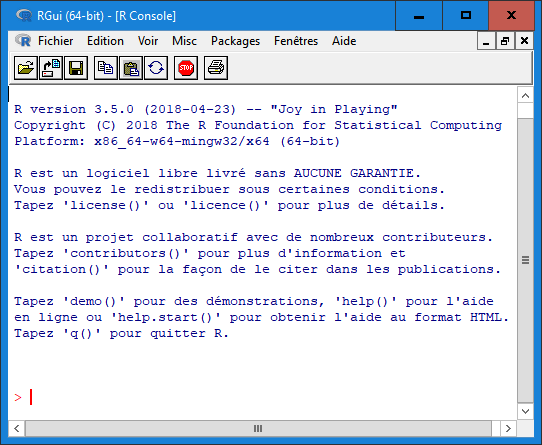
\includegraphics{myFigures/screencap_rConsoleFR.png}
\caption{\label{fig:screenCapConsole}Capture d'écran de la console R sous
Windows.\label{fig:screenCapConsole}}
\end{figure}

La console correspond à l'interface où va être interprété le code, c'est
à dire à l'endroit où le code va être transformé en langage machine,
éxécuter par l'ordinateur, puis retransmis sous une forme lisible par
des humains. Cela correspond à l'écran d'affichage d'une calculatrice
(Figure \ref{fig:screenCapConsoleCal}). C'est de cette manière que R va
être utilisé dans la suite de cette section.

\begin{rmdnote}
Tout au long de ce livre, les exemples de code R apparaîtront sur fond
en gris. Ils peuvent être copiés et collés directement dans la console,
bien qu'il soit préférable de reproduire soit même les exemples dans la
console (ou plus tard dans les scripts). Le résultat de ce qui est
envoyé dans la console apparaîtra également sur fond en gris avec
\texttt{\#\#} devant le code afin de bien faire la distinction entre le
code et le résultat du code.
\end{rmdnote}

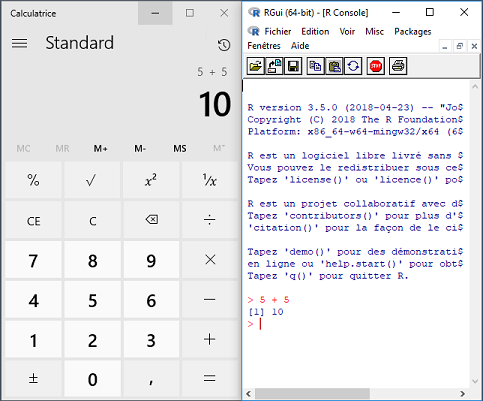
\includegraphics{myFigures/screencap_rConsoleCalculatrice.png} \#\#\#
Les opérateurs arithmétiques

\begin{Shaded}
\begin{Highlighting}[]
\DecValTok{5} \OperatorTok{+}\StringTok{ }\DecValTok{5}
\end{Highlighting}
\end{Shaded}

\begin{verbatim}
## [1] 10
\end{verbatim}

Si nous écrivons \texttt{5\ +\ 5} dans la console puis \texttt{Entrée},
le résultat apparaît précédé du chiffre {[}1{]} entre crochets. Ce
chiffre correspond au numéro du résultat (dans notre cas, il n'y a qu'un
seul résultat ; nous reviendrons sur cet aspect plus tard). Nous pouvons
également noter dans cet exemple l'utilisation d'espaces avant et après
le signe \texttt{+}. Ces espaces ne sont pas nécessaires mais permettent
au code d'être plus lisible par les humains (i.e., plus agréable à lire
pour nous comme pour les personnes avec qui nous serons amenés à
partager notre code). Les opérateurs aritmétiques disponibles sous R
sont résumés dans la table \ref{tab:tabOpAri}.

\begin{table}

\caption{\label{tab:tabOpAri}Opérateurs arithmétiques.\label{tab:tabOpAri}}
\centering
\begin{tabular}[t]{l|l}
\hline
Label & Operateur\\
\hline
Addition & +\\
\hline
Soustraction & -\\
\hline
Multiplication & *\\
\hline
Division & /\\
\hline
Puissance & \textasciicircum{}\\
\hline
Modulo & \%\%\\
\hline
Quotien Décimal & \%/\%\\
\hline
\end{tabular}
\end{table}

Classiquement, les multiplications et les divisions sont prioritaires
sur les additions et les soustractions. Au besoin nous pouvons utiliser
des parenthèses.

\begin{Shaded}
\begin{Highlighting}[]
\DecValTok{5} \OperatorTok{+}\StringTok{ }\DecValTok{5} \OperatorTok{*}\StringTok{ }\DecValTok{2}
\end{Highlighting}
\end{Shaded}

\begin{verbatim}
## [1] 15
\end{verbatim}

\begin{Shaded}
\begin{Highlighting}[]
\NormalTok{(}\DecValTok{5} \OperatorTok{+}\StringTok{ }\DecValTok{5}\NormalTok{) }\OperatorTok{*}\StringTok{ }\DecValTok{2}
\end{Highlighting}
\end{Shaded}

\begin{verbatim}
## [1] 20
\end{verbatim}

L'opérateur modulo correspond au reste de la division euclidienne. Il
est souvent utilisé en informatique par exemple pour savoir si un nombre
est pair ou impair (un nombre modulo 2 va renvoyer 1 si il est impair et
0 si il est pair).

\begin{Shaded}
\begin{Highlighting}[]
\DecValTok{451} \OperatorTok\StringTok{ }\DecValTok{2}
\end{Highlighting}
\end{Shaded}

\begin{verbatim}
## [1] 1
\end{verbatim}

\begin{Shaded}
\begin{Highlighting}[]
\DecValTok{288} \OperatorTok\StringTok{ }\DecValTok{2}
\end{Highlighting}
\end{Shaded}

\begin{verbatim}
## [1] 0
\end{verbatim}

\begin{Shaded}
\begin{Highlighting}[]
\NormalTok{(}\DecValTok{5} \OperatorTok{+}\StringTok{ }\DecValTok{5} \OperatorTok{*}\StringTok{ }\DecValTok{2}\NormalTok{) }\OperatorTok\StringTok{ }\DecValTok{2}
\end{Highlighting}
\end{Shaded}

\begin{verbatim}
## [1] 1
\end{verbatim}

\begin{Shaded}
\begin{Highlighting}[]
\NormalTok{((}\DecValTok{5} \OperatorTok{+}\StringTok{ }\DecValTok{5}\NormalTok{) }\OperatorTok{*}\StringTok{ }\DecValTok{2}\NormalTok{) }\OperatorTok\StringTok{ }\DecValTok{2}
\end{Highlighting}
\end{Shaded}

\begin{verbatim}
## [1] 0
\end{verbatim}

R intègre également certaines constantes dont \texttt{pi}. Par ailleurs
le signe infini est représenté par \texttt{Inf}

\begin{Shaded}
\begin{Highlighting}[]
\NormalTok{pi}
\end{Highlighting}
\end{Shaded}

\begin{verbatim}
## [1] 3.141593
\end{verbatim}

\begin{Shaded}
\begin{Highlighting}[]
\NormalTok{pi }\OperatorTok{*}\StringTok{ }\DecValTok{5}\OperatorTok{^}\DecValTok{2}
\end{Highlighting}
\end{Shaded}

\begin{verbatim}
## [1] 78.53982
\end{verbatim}

\begin{Shaded}
\begin{Highlighting}[]
\DecValTok{1}\OperatorTok{/}\DecValTok{0}
\end{Highlighting}
\end{Shaded}

\begin{verbatim}
## [1] Inf
\end{verbatim}

\begin{rmdstyle}
le \emph{style} du code est important car le code est destiné à être
lisible par nous plus tard et par d'autres personnes de manière
générale. Pour avoir un style lisible il est recommandé de mettre des
espaces avant et après les opérateurs arithmétiques. Les informations
concernant le \emph{style} seront toujours représentées avec ce
pictogramme afin qu'elles soient facilement identifiables.
\end{rmdstyle}

\subsection{Les opérateurs de
comparaison}\label{les-operateurs-de-comparaison}

R est cependant bien plus qu'une simple calculatrice puisque'il permet
un autre type d'opérateurs : les opérateurs de comparaison. Ils servent
comme leur nom l'indique à \emph{comparer} des valeurs entre elles
(Table \ref{tab:tabOpCom}).

\begin{table}

\caption{\label{tab:tabOpCom}Opérateurs de comparaison.\label{tab:tabOpCom}}
\centering
\begin{tabular}[t]{l|l}
\hline
Label & Operador\\
\hline
plus petit que & <\\
\hline
plus grand que & >\\
\hline
plus petit ou égal à & <=\\
\hline
plus grand ou égal à & >=\\
\hline
égal à & ==\\
\hline
différent de & !=\\
\hline
\end{tabular}
\end{table}

Par exemple si nous voulons savoir si un chiffre est plus grand qu'un
autre, nous pouvons écrire :

\begin{Shaded}
\begin{Highlighting}[]
\DecValTok{5} \OperatorTok{>}\StringTok{ }\DecValTok{3} 
\end{Highlighting}
\end{Shaded}

\begin{verbatim}
## [1] TRUE
\end{verbatim}

R renvoie la valeur \texttt{TRUE} si la comparasion est vraie et
\texttt{FALSE} si la comparaison est fausse.

\begin{Shaded}
\begin{Highlighting}[]
\DecValTok{5} \OperatorTok{>}\StringTok{ }\DecValTok{3}
\end{Highlighting}
\end{Shaded}

\begin{verbatim}
## [1] TRUE
\end{verbatim}

\begin{Shaded}
\begin{Highlighting}[]
\DecValTok{2} \OperatorTok{<}\StringTok{ }\FloatTok{1.5}
\end{Highlighting}
\end{Shaded}

\begin{verbatim}
## [1] FALSE
\end{verbatim}

\begin{Shaded}
\begin{Highlighting}[]
\DecValTok{2} \OperatorTok{<=}\StringTok{ }\DecValTok{2}
\end{Highlighting}
\end{Shaded}

\begin{verbatim}
## [1] TRUE
\end{verbatim}

\begin{Shaded}
\begin{Highlighting}[]
\FloatTok{3.2} \OperatorTok{>=}\StringTok{ }\FloatTok{1.5}
\end{Highlighting}
\end{Shaded}

\begin{verbatim}
## [1] TRUE
\end{verbatim}

Nous pouvons combiner les opérateurs arithmétiques avec les opérateurs
de comparasion.

\begin{Shaded}
\begin{Highlighting}[]
\NormalTok{(}\DecValTok{5} \OperatorTok{+}\StringTok{ }\DecValTok{8}\NormalTok{) }\OperatorTok{>}\StringTok{ }\NormalTok{(}\DecValTok{3} \OperatorTok{*}\StringTok{ }\DecValTok{45}\OperatorTok{/}\DecValTok{2}\NormalTok{) }
\end{Highlighting}
\end{Shaded}

\begin{verbatim}
## [1] FALSE
\end{verbatim}

\begin{rmdstyle}
Dans la comparasion \texttt{(5\ +\ 8)\ \textgreater{}\ (3\ *\ 45/2)} les
parenthèses ne sont pas nécessaires mais elles permettent au code d'être
plus facile à lire.
\end{rmdstyle}

Un opérateur de comparaison particulier est \emph{égal à}. Nous verrons
dans la section suivante que le signe \texttt{=} est réservé à un autre
usage : il permet d'affecter une valeur à un objet. L'opérateur de
comparaison \emph{égal à} doit donc être différent, c'est pour cela que
R utilise \texttt{==}.

\begin{Shaded}
\begin{Highlighting}[]
\DecValTok{42} \OperatorTok{==}\StringTok{ }\DecValTok{53}
\end{Highlighting}
\end{Shaded}

\begin{verbatim}
## [1] FALSE
\end{verbatim}

\begin{Shaded}
\begin{Highlighting}[]
\DecValTok{58} \OperatorTok{==}\StringTok{ }\DecValTok{58}
\end{Highlighting}
\end{Shaded}

\begin{verbatim}
## [1] TRUE
\end{verbatim}

Un autre opérateur particulier est \emph{différent de}. Il est utilisé
avec \emph{un point d'intérrogation} suivi de \emph{égal}, \texttt{!=}.
Cet opérateur permet de d'obtenir la réponse inverse à \texttt{==}.

\begin{Shaded}
\begin{Highlighting}[]
\DecValTok{42} \OperatorTok{==}\StringTok{ }\DecValTok{53}
\end{Highlighting}
\end{Shaded}

\begin{verbatim}
## [1] FALSE
\end{verbatim}

\begin{Shaded}
\begin{Highlighting}[]
\DecValTok{42} \OperatorTok{!=}\StringTok{ }\DecValTok{53}
\end{Highlighting}
\end{Shaded}

\begin{verbatim}
## [1] TRUE
\end{verbatim}

\begin{Shaded}
\begin{Highlighting}[]
\NormalTok{(}\DecValTok{3} \OperatorTok{+}\StringTok{ }\DecValTok{2}\NormalTok{) }\OperatorTok{!=}\StringTok{ }\DecValTok{5}
\end{Highlighting}
\end{Shaded}

\begin{verbatim}
## [1] FALSE
\end{verbatim}

\begin{Shaded}
\begin{Highlighting}[]
\DecValTok{10}\OperatorTok{/}\DecValTok{2} \OperatorTok{==}\StringTok{ }\DecValTok{5}
\end{Highlighting}
\end{Shaded}

\begin{verbatim}
## [1] TRUE
\end{verbatim}

R utilise \texttt{TRUE} et \texttt{FALSE} qui sont aussi des valeurs qui
peuvent être testées avec les opérateurs de comparasion. Mais R attribue
également une valeur à \texttt{TRUE} et \texttt{FALSE} :

\begin{Shaded}
\begin{Highlighting}[]
\OtherTok{TRUE} \OperatorTok{==}\StringTok{ }\OtherTok{TRUE}
\end{Highlighting}
\end{Shaded}

\begin{verbatim}
## [1] TRUE
\end{verbatim}

\begin{Shaded}
\begin{Highlighting}[]
\OtherTok{TRUE} \OperatorTok{>}\StringTok{ }\OtherTok{FALSE}
\end{Highlighting}
\end{Shaded}

\begin{verbatim}
## [1] TRUE
\end{verbatim}

\begin{Shaded}
\begin{Highlighting}[]
\DecValTok{1} \OperatorTok{==}\StringTok{ }\OtherTok{TRUE}
\end{Highlighting}
\end{Shaded}

\begin{verbatim}
## [1] TRUE
\end{verbatim}

\begin{Shaded}
\begin{Highlighting}[]
\DecValTok{0} \OperatorTok{==}\StringTok{ }\OtherTok{FALSE}
\end{Highlighting}
\end{Shaded}

\begin{verbatim}
## [1] TRUE
\end{verbatim}

\begin{Shaded}
\begin{Highlighting}[]
\OtherTok{TRUE} \OperatorTok{+}\StringTok{ }\DecValTok{1}
\end{Highlighting}
\end{Shaded}

\begin{verbatim}
## [1] 2
\end{verbatim}

\begin{Shaded}
\begin{Highlighting}[]
\OtherTok{FALSE} \OperatorTok{+}\StringTok{ }\DecValTok{1}
\end{Highlighting}
\end{Shaded}

\begin{verbatim}
## [1] 1
\end{verbatim}

\begin{Shaded}
\begin{Highlighting}[]
\NormalTok{(}\OtherTok{FALSE} \OperatorTok{+}\StringTok{ }\DecValTok{1}\NormalTok{) }\OperatorTok{==}\StringTok{ }\OtherTok{TRUE}
\end{Highlighting}
\end{Shaded}

\begin{verbatim}
## [1] TRUE
\end{verbatim}

La valeur de \texttt{TRUE} est de 1 et la valeur de \texttt{FALSE} est
de 0. Nous verrons plus tard comment utiliser cette information dans les
prochains chapitres.

R est aussi un langage relativement permissif, cela veut dire qu'il
admet une certaine flexibilité dans la manière de rédiger le code.
Débattre du bien fondé de cette flexibilité sort du cadre de ce livre
mais nous pourrons trouver dans du code R sur Internet ou dans d'autres
ouvrages le raccourcis \texttt{T} pour \texttt{TRUE} et \texttt{F} pour
\texttt{FALSE}.

\begin{Shaded}
\begin{Highlighting}[]
\NormalTok{T }\OperatorTok{==}\StringTok{ }\OtherTok{TRUE}
\end{Highlighting}
\end{Shaded}

\begin{verbatim}
## [1] TRUE
\end{verbatim}

\begin{Shaded}
\begin{Highlighting}[]
\NormalTok{F }\OperatorTok{==}\StringTok{ }\OtherTok{FALSE}
\end{Highlighting}
\end{Shaded}

\begin{verbatim}
## [1] TRUE
\end{verbatim}

\begin{Shaded}
\begin{Highlighting}[]
\NormalTok{T }\OperatorTok{==}\StringTok{ }\DecValTok{1}
\end{Highlighting}
\end{Shaded}

\begin{verbatim}
## [1] TRUE
\end{verbatim}

\begin{Shaded}
\begin{Highlighting}[]
\NormalTok{F }\OperatorTok{==}\StringTok{ }\DecValTok{0}
\end{Highlighting}
\end{Shaded}

\begin{verbatim}
## [1] TRUE
\end{verbatim}

\begin{Shaded}
\begin{Highlighting}[]
\NormalTok{(F }\OperatorTok{+}\StringTok{ }\DecValTok{1}\NormalTok{) }\OperatorTok{==}\StringTok{ }\OtherTok{TRUE}
\end{Highlighting}
\end{Shaded}

\begin{verbatim}
## [1] TRUE
\end{verbatim}

Bien que cette façon de se référer à \texttt{TRUE} et \texttt{FALSE} par
\texttt{T} et \texttt{F} soit assez répandue, dans ce livre nous
utiliserons toujours \texttt{TRUE} et \texttt{FALSE} afin que le code
soit plus facile à lire. Encore une fois l'objectif d'un code est de non
seuleument être fonctionnel mais aussi d'être facile à lire et à relire.

\subsection{Les opérateurs logiques}\label{les-operateurs-logiques}

Il existe un dernier type d'opérateur, les opérateurs logiques. Ils sont
utiles pour combiner des opérateurs de comparaison (Table
\ref{tab:tabOpLog}).

\begin{table}

\caption{\label{tab:tabOpLog}Opérateurs logiques.\label{tab:tabOpLog}}
\centering
\begin{tabular}[t]{l|l}
\hline
Label & Operador\\
\hline
n'est pas & !\\
\hline
et & \&\\
\hline
ou & |\\
\hline
ou exclusif & xor()\\
\hline
\end{tabular}
\end{table}

\begin{Shaded}
\begin{Highlighting}[]
\OperatorTok{!}\OtherTok{TRUE}
\end{Highlighting}
\end{Shaded}

\begin{verbatim}
## [1] FALSE
\end{verbatim}

\begin{Shaded}
\begin{Highlighting}[]
\OperatorTok{!}\OtherTok{FALSE}
\end{Highlighting}
\end{Shaded}

\begin{verbatim}
## [1] TRUE
\end{verbatim}

\begin{Shaded}
\begin{Highlighting}[]
\NormalTok{((}\DecValTok{3} \OperatorTok{+}\StringTok{ }\DecValTok{2}\NormalTok{) }\OperatorTok{==}\StringTok{ }\DecValTok{5}\NormalTok{) }\OperatorTok{&}\StringTok{ }\NormalTok{((}\DecValTok{3} \OperatorTok{+}\StringTok{ }\DecValTok{3}\NormalTok{) }\OperatorTok{==}\StringTok{ }\DecValTok{5}\NormalTok{)}
\end{Highlighting}
\end{Shaded}

\begin{verbatim}
## [1] FALSE
\end{verbatim}

\begin{Shaded}
\begin{Highlighting}[]
\NormalTok{((}\DecValTok{3} \OperatorTok{+}\StringTok{ }\DecValTok{2}\NormalTok{) }\OperatorTok{==}\StringTok{ }\DecValTok{5}\NormalTok{) }\OperatorTok{&}\StringTok{ }\NormalTok{((}\DecValTok{3} \OperatorTok{+}\StringTok{ }\DecValTok{3}\NormalTok{) }\OperatorTok{==}\StringTok{ }\DecValTok{6}\NormalTok{)}
\end{Highlighting}
\end{Shaded}

\begin{verbatim}
## [1] TRUE
\end{verbatim}

\begin{Shaded}
\begin{Highlighting}[]
\NormalTok{(}\DecValTok{3} \OperatorTok{<}\StringTok{ }\DecValTok{5}\NormalTok{) }\OperatorTok{&}\StringTok{ }\NormalTok{(}\DecValTok{5} \OperatorTok{<}\StringTok{ }\DecValTok{5}\NormalTok{)}
\end{Highlighting}
\end{Shaded}

\begin{verbatim}
## [1] FALSE
\end{verbatim}

\begin{Shaded}
\begin{Highlighting}[]
\NormalTok{(}\DecValTok{3} \OperatorTok{<}\StringTok{ }\DecValTok{5}\NormalTok{) }\OperatorTok{&}\StringTok{ }\NormalTok{(}\DecValTok{5} \OperatorTok{<=}\StringTok{ }\DecValTok{5}\NormalTok{)}
\end{Highlighting}
\end{Shaded}

\begin{verbatim}
## [1] TRUE
\end{verbatim}

L'opérateur logique \texttt{xor()} correspond à un \emph{ou exclusif}.
C'est à dire que l'un des deux \textbf{arguments} de la
\textbf{fonction} \texttt{xor()} doit être vrai, mais pas les deux. Nous
reviendrons plus tard sur les \textbf{fonctions} et leurs
\textbf{arguments}, mais retenons que l'on identifie une fonction par
ses parenthèses qui contiennent des arguments séparés par des virgules.

\begin{Shaded}
\begin{Highlighting}[]
\KeywordTok{xor}\NormalTok{((}\DecValTok{3} \OperatorTok{+}\StringTok{ }\DecValTok{2}\NormalTok{) }\OperatorTok{==}\StringTok{ }\DecValTok{5}\NormalTok{, (}\DecValTok{3} \OperatorTok{+}\StringTok{ }\DecValTok{3}\NormalTok{) }\OperatorTok{==}\StringTok{ }\DecValTok{6}\NormalTok{)}
\end{Highlighting}
\end{Shaded}

\begin{verbatim}
## [1] FALSE
\end{verbatim}

\begin{Shaded}
\begin{Highlighting}[]
\KeywordTok{xor}\NormalTok{((}\DecValTok{3} \OperatorTok{+}\StringTok{ }\DecValTok{2}\NormalTok{) }\OperatorTok{==}\StringTok{ }\DecValTok{5}\NormalTok{, (}\DecValTok{3} \OperatorTok{+}\StringTok{ }\DecValTok{2}\NormalTok{) }\OperatorTok{==}\StringTok{ }\DecValTok{6}\NormalTok{)}
\end{Highlighting}
\end{Shaded}

\begin{verbatim}
## [1] TRUE
\end{verbatim}

\begin{Shaded}
\begin{Highlighting}[]
\KeywordTok{xor}\NormalTok{((}\DecValTok{3} \OperatorTok{+}\StringTok{ }\DecValTok{3}\NormalTok{) }\OperatorTok{==}\StringTok{ }\DecValTok{5}\NormalTok{, (}\DecValTok{3} \OperatorTok{+}\StringTok{ }\DecValTok{2}\NormalTok{) }\OperatorTok{==}\StringTok{ }\DecValTok{6}\NormalTok{)}
\end{Highlighting}
\end{Shaded}

\begin{verbatim}
## [1] FALSE
\end{verbatim}

\begin{Shaded}
\begin{Highlighting}[]
\KeywordTok{xor}\NormalTok{((}\DecValTok{3} \OperatorTok{+}\StringTok{ }\DecValTok{3}\NormalTok{) }\OperatorTok{==}\StringTok{ }\DecValTok{5}\NormalTok{, (}\DecValTok{3} \OperatorTok{+}\StringTok{ }\DecValTok{3}\NormalTok{) }\OperatorTok{==}\StringTok{ }\DecValTok{6}\NormalTok{)}
\end{Highlighting}
\end{Shaded}

\begin{verbatim}
## [1] TRUE
\end{verbatim}

\begin{rmdstyle}
Il est recommandé que les virgules \texttt{,} soient suivies par un
espace afin que le code soit plus agréable à lire.
\end{rmdstyle}

\subsection{Aide sur les opérateurs}\label{aide-sur-les-operateurs}

Le fichier d'aideen anglais sur les opérateurs arithmétiques peut être
obtenue avec la commande \texttt{?\textquotesingle{}+\textquotesingle{}}
celui sur les opérateurs de comparaison avec la commande
\texttt{?\textquotesingle{}==\textquotesingle{}} et celui sur les
opérateurs logiques avec la commande
\texttt{?\textquotesingle{}\&\textquotesingle{}}.

\section{La notion d'objet}\label{la-notion-dobjet}

Un aspect important de la programmation avec R, mais aussi de la
programmation en général est la notion d'objet. Comme indiqué sur la
page web de wikipedia
(\url{https://fr.wikipedia.org/wiki/Objet_(informatique)}), en
informatique, un objet est un \emph{conteneur}, c'est à dire quelque
chose qui va contenir de l'information. L'inforamtion contenue dans un
objet peut être très diverse, mais pour le moment nous allons contenir
dans un objet le chiffre 5. Pour ce faire (et pour pouvoir le réutiliser
par la suite), il nous faut donner un nom à notre objet. Avec R le nom
des objets ne doit pas comprendre de caractères spéciaux comme
\emph{\^{}\$?\textbar{}+(){[}{]}\}\{}, ne doit pas commencer par un
chiffre ni contenir d'espaces. Le nom de l'objet doit être représentatif
de ce qu'il contient, tout en étant ni trop court ni trop long.
Imaginons que notre chiffre 5 corresponde au nombre de répétitions d'une
expérience. Nous voudrions lui donner un nom faisant référence à
\emph{nombre} et à \emph{répétition}, que nous pourrions réduire à
\emph{nbr} et \emph{rep}, respectivement. Il existe plusieurs
possibilités qui sont toutes assez répandues sous R :

\begin{itemize}
\tightlist
\item
  la séparation au moyen du caractère \emph{tiret bas} :
  \texttt{nbr\_rep}
\item
  la séparation au moyen du caractère \emph{point} : \texttt{nbr.rep}
\item
  l'utilisation de lettres minuscules : \texttt{nbrrep}
\item
  le style \emph{lowerCamelCase} consistant en un premier mot en
  minuscules et des suivants avec une majuscule : \texttt{nbrRep}
\item
  le style \emph{UpperCamelCase} consistant à mettre une majuscule au
  début de chacun des mots : \texttt{NbrRep}
\end{itemize}

Toutes ces formes de nommer un objet sont équivalentes. Dans ce livre
nous utiliserons le style \emph{lowerCamelCase}. De manière générale il
faut éviter les noms trop longs comme \texttt{leNombreDeRepetitions} ou
trop courts comme \texttt{nR}, et les noms ne permettant pas
d'identifier le contenu comme \texttt{maVariable} ou
\texttt{monChiffre}, mais aussi \texttt{a} ou \texttt{b}\ldots{}

\begin{rmdstyle}
Il existe différentes façons de définir un nom pour les objets que nous
allons créer avec R. Dans ce livre il est utilisé le style
\emph{lowerCamelCase}. L'important n'est pas le choix du style mais la
consistence dans son choix. L'objectif est d'avoir un code fonctionnel
mais également un code facile et agréable à lire.
\end{rmdstyle}

Maintenant que nous avons choisi un nom pour notre objet, il faut le
créer et faire comprendre à R que notre objet doit contenir le chiffre
5. Il existe trois façons de créer un objet sous R:

\begin{itemize}
\tightlist
\item
  avec le signe \texttt{\textless{}-}
\item
  avec le signe \texttt{=}
\item
  avec le signe \texttt{-\textgreater{}}
\end{itemize}

\begin{Shaded}
\begin{Highlighting}[]
\NormalTok{nbrRep <-}\StringTok{ }\DecValTok{5}
\NormalTok{nbrRep =}\StringTok{ }\DecValTok{5}
\DecValTok{5}\NormalTok{ ->}\StringTok{ }\NormalTok{nbrRep}
\end{Highlighting}
\end{Shaded}

Dans ce livre nous utiliserons toujours la forme \texttt{\textless{}-}
par souci de consistence et aussi parce que c'est la forme la plus
répendue.

\begin{Shaded}
\begin{Highlighting}[]
\NormalTok{nbrRep <-}\StringTok{ }\DecValTok{5}
\end{Highlighting}
\end{Shaded}

Nous venons de créer un objet \texttt{nbrRep} et de lui affecter la
valeur 5. Cet objet est désormais disponible dans notre environnement de
calcul et peut donc être utilisé. Voici quelques exemples :

\begin{Shaded}
\begin{Highlighting}[]
\NormalTok{nbrRep }\OperatorTok{+}\StringTok{ }\DecValTok{2}
\end{Highlighting}
\end{Shaded}

\begin{verbatim}
## [1] 7
\end{verbatim}

\begin{Shaded}
\begin{Highlighting}[]
\NormalTok{nbrRep }\OperatorTok{*}\StringTok{ }\DecValTok{5} \OperatorTok{-}\StringTok{ }\DecValTok{45}\OperatorTok{/}\DecValTok{56}
\end{Highlighting}
\end{Shaded}

\begin{verbatim}
## [1] 24.19643
\end{verbatim}

\begin{Shaded}
\begin{Highlighting}[]
\NormalTok{pi }\OperatorTok{*}\StringTok{ }\NormalTok{nbrRep}\OperatorTok{^}\DecValTok{2}
\end{Highlighting}
\end{Shaded}

\begin{verbatim}
## [1] 78.53982
\end{verbatim}

La valeur associée à notre objet \texttt{nbrRep} peut être modifiée de
la même manière que lors de sa création :

\begin{Shaded}
\begin{Highlighting}[]
\NormalTok{nbrRep <-}\StringTok{ }\DecValTok{5}
\NormalTok{nbrRep }\OperatorTok{+}\StringTok{ }\DecValTok{2}
\end{Highlighting}
\end{Shaded}

\begin{verbatim}
## [1] 7
\end{verbatim}

\begin{Shaded}
\begin{Highlighting}[]
\NormalTok{nbrRep <-}\StringTok{ }\DecValTok{10}
\NormalTok{nbrRep }\OperatorTok{+}\StringTok{ }\DecValTok{2}
\end{Highlighting}
\end{Shaded}

\begin{verbatim}
## [1] 12
\end{verbatim}

\begin{Shaded}
\begin{Highlighting}[]
\NormalTok{nbrRep <-}\StringTok{ }\DecValTok{5} \OperatorTok{*}\StringTok{ }\DecValTok{2} \OperatorTok{+}\StringTok{ }\DecValTok{7}\OperatorTok{/}\DecValTok{3}
\NormalTok{nbrRep }\OperatorTok{+}\StringTok{ }\DecValTok{2}
\end{Highlighting}
\end{Shaded}

\begin{verbatim}
## [1] 14.33333
\end{verbatim}

L'utilisation des objets prend tout son sens lorsque nous avons des
opérations complexes à réaliser et rend le code plus agréable à lire et
à comprendre.

\begin{Shaded}
\begin{Highlighting}[]
\NormalTok{(}\DecValTok{5} \OperatorTok{+}\StringTok{ }\DecValTok{9}\OperatorTok{^}\DecValTok{2} \OperatorTok{-}\StringTok{ }\DecValTok{1}\OperatorTok{/}\DecValTok{18}\NormalTok{) }\OperatorTok{/}\StringTok{ }\NormalTok{(}\DecValTok{32} \OperatorTok{*}\StringTok{ }\DecValTok{45}\OperatorTok{/}\DecValTok{8} \OperatorTok{+}\StringTok{ }\DecValTok{3}\NormalTok{)}
\end{Highlighting}
\end{Shaded}

\begin{verbatim}
## [1] 0.4696418
\end{verbatim}

\begin{Shaded}
\begin{Highlighting}[]
\NormalTok{terme01 <-}\StringTok{ }\DecValTok{5} \OperatorTok{+}\StringTok{ }\DecValTok{9}\OperatorTok{^}\DecValTok{2} \OperatorTok{-}\StringTok{ }\DecValTok{1}\OperatorTok{/}\DecValTok{18}
\NormalTok{terme02 <-}\StringTok{ }\DecValTok{32} \OperatorTok{*}\StringTok{ }\DecValTok{45}\OperatorTok{/}\DecValTok{8} \OperatorTok{+}\StringTok{ }\DecValTok{3}
\NormalTok{terme01 }\OperatorTok{/}\StringTok{ }\NormalTok{terme02}
\end{Highlighting}
\end{Shaded}

\begin{verbatim}
## [1] 0.4696418
\end{verbatim}

\section{Les scripts}\label{les-scripts}

R est un langage de programmation souvent dénommé \emph{langage de
script}. Cela fait référence au fait que la plupart des utilisateurs
vont écrire des petits bouts de code plutôt que des programmes entiers.
R peut être utilisé comme une simple calculatrice, et dans ce cas il ne
sera pas nécessaire de conserver un historique des opérations qui ont
été réalisées. Mais si les opérations à réliser sont longues et
complexes, il peut devenir nécessaire de pouvoir sauvegarder ce qui a
été fait à un moment donné pour pouvoir poursuivre plus tard. Le fichier
dans lequel seront conservées les opérations consitue ce que l'on
appelle communement le script. Un script est donc un fichier contenant
une succession d'informations compréhensibles par R et qu'il est
possible d'éxécuter.

\subsection{Créer un script et le
documenter}\label{creer-un-script-et-le-documenter}

Pour ouvrir un nouveau script il suffit de créer un fichier texte vide
qui sera édité par un éditeur de texte comme le bloc note sous Windows
ou Mac OS, ou encore Gedit ou même nano sous Linux. Par convention ce
fichier prend l'extension ``.r'' ou plus souvent ``.R''. C'est cette
dernière convention qui sera utilisée dans ce livre. Depuis l'interface
graphique de R il est possible de créer un nouveux script sous Mac OS et
Windows via \emph{fichier} puis \emph{nouveau script} et
\emph{enregistrer sous}. Tout comme le nom des objets, le nom du script
est important pour que nous puissions facilement identifier son contenu.
Par exemple nous pourrions créer un fichier \texttt{formRConceptsBase.R}
contenant les objets que nous venons de créer et les calculs effectués.
Mais même avec des noms de variables et un nom de fichier bien définis,
il sera difficile de se rappeler le sens de cce fichier sans une
documentation accompagnant ce script. Pour docummenter un script nous
allons utiliser des \emph{commentaires}. Les commentaires sont des
éléments qui seront identifiés par R comme tel et qui ne seront pas
éxécutés. Pour spécifier à R que nous allons faire un commentaire, il
faut utiliser le caractère octothorpe (croisillon) \texttt{\#}. Les
commentaires peuvent être insérés sur une nouvelle ligne ou en fin de
ligne.

\begin{Shaded}
\begin{Highlighting}[]
\CommentTok{# creation objet nombre de repetitions}
\NormalTok{nbrRep <-}\StringTok{ }\DecValTok{5} \CommentTok{# commentaire de fin de ligne}
\end{Highlighting}
\end{Shaded}

Les commentaires peuvent aussi être utilisé pour qu'une ligne ne soit
plus éxécutée.

\begin{Shaded}
\begin{Highlighting}[]
\NormalTok{nbrRep <-}\StringTok{ }\DecValTok{5}
\CommentTok{# nbrRep + 5}
\end{Highlighting}
\end{Shaded}

Pour en revenir à la documentation du script, il est recommandé de
commencer chacun de ses scripts par une brève description de son
contenu, puis lorsque le script devient long, de le structurer en
différentes parties pour faciliter sa lecture.

\begin{Shaded}
\begin{Highlighting}[]
\CommentTok{# ------------------------------------------------------------}
\CommentTok{# Voici un script pour acquérir les concepts de base }
\CommentTok{# avec R}
\CommentTok{# date de création : 25/06/2018}
\CommentTok{# auteur : François Rebaudo}
\CommentTok{# ------------------------------------------------------------}

\CommentTok{# [1] création de l'objet nombre de répétitions}
\CommentTok{# ------------------------------------------------------------}

\NormalTok{nbrRep <-}\StringTok{ }\DecValTok{5}

\CommentTok{# [2] calculs simples}
\CommentTok{# ------------------------------------------------------------}

\NormalTok{pi }\OperatorTok{*}\StringTok{ }\NormalTok{nbrRep}\OperatorTok{^}\DecValTok{2}
\end{Highlighting}
\end{Shaded}

\begin{verbatim}
## [1] 78.53982
\end{verbatim}

\begin{rmdstyle}
Pour aller plus loin sur le style de code, un guide complet de
recommandations est disponible en ligne (en anglais ;
\url{http://style.tidyverse.org/}).
\end{rmdstyle}

\subsection{Exécuter un script}\label{executer-un-script}

Depuis que nous avons un script, nous ne travaillons plus directement
dans la console. Or seule la console est capable d'interpérter le code R
et de nous renvoyer les résultats que nous souhaitons obtenir. Pour
l'instant la technique la plus simple consiste à copier-coller les
lignes que nous souhaitons éxécuter depuis notre script vers la console.
A partir de maintenant nous n'allons plus utiliser les éditeurs de texte
comme le bloc note mais des éditeurs spécialisés pour la confection de
scripts R. C'est l'objet du chapitre suivant.

\chapter{Choisir un environnement de développement}\label{IDE}

\section{Editeurs de texte et environnement de
développement}\label{editeurs-de-texte-et-environnement-de-developpement}

Il existe de très nombreux éditeurs de texte, le chapitre précédent a
permit d'en introduire quelque uns parmis les plus simples comme le bloc
note de Windows. Rapidement les limites de ces éditeurs ont rendu la
tâche d'écrire un script fastidieuse. En effet, même en structurant son
script avec des commentaires, il reste difficile de se répérer dans
celui-ci. C'est là qu'interviennent les éditeurs de texte spécialisés
qui vont permettre une écriture et une lecture agréable et simplifiée.
L'éditeur de texte pour R certqinement le plus répandu est Rstudio, mais
il en existe bien d'autres. Faire une liste exhaustive de toutes les
solutions disponibles sort du cadre de ce livre, ainsi nous nous
focaliserons sur les trois solutions que j'utilise au quotidien que sont
\textbf{Notepad++}, \textbf{Rstudio}, et \textbf{Geany}.

\section{RStudio}\label{rstudio}

\begin{figure}
\centering

\includegraphics{myLogos/RStudio.png}
\caption{\label{fig:logoRStudio}Logo RStudio.\label{fig:logoRStudio}}
\end{figure}

\subsection{Installer RStudio}\label{installer-rstudio}

Le programme pour installer Rstudio se retrouve dans la partie
\emph{Products} du site web de Rstudio (\url{https://www.rstudio.com/}).
Nous allons installé RStudio pour un usage local (sur notre ordinateur),
donc la version qui nous intéresse est \emph{Desktop}. Nous allons
utiliser la version \emph{Open Source} qui est gratuite. Ensuite il nous
suffit de sélectionner la version qui correspond à notre système
d'exploitation, de télécharger le fichier correspondant et de l'exécuter
pour lancer l'installation. Nous pouvons conserver les options par
défaut tout au long de l'installation.

\subsection{Un script avec RStudio}\label{un-script-avec-rstudio}

Nous pouvons alors ouvrir RStudio. Lors de la première ouverture,
l'interface est divisée en deux avec à gauche la console R que nous
avons vu au chapitre précédent (Figure \ref{fig:screenCapRStudio01}).
Pour ouvrir un nouveau script, nous allons dans le menu \emph{File},
\emph{New File}, \emph{R script}. Par défaut ce fichier a comme nom
\emph{Untitled1}. Nous avons vu au chapitre précédent l'importance de
donner un nom pertinent à nos scripts, c'est pourquoi nous allons le
renommer \emph{selecEnvDev.R}, dans le menu \emph{File}, avec l'option
\emph{Save As\ldots{}}. Nous avons pu noter que la partie gauche de
RStudio est désormais séparée en deux, avec en bas de l'écran la console
et en haut de l'écran le script.

\begin{figure}
\centering
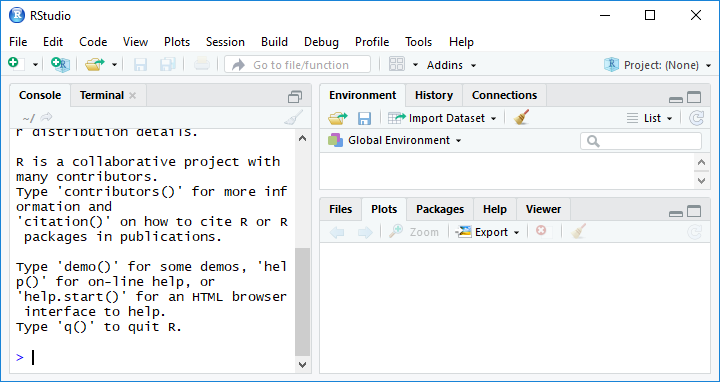
\includegraphics{myFigures/screencap_RStudio_01.png}
\caption{\label{fig:screenCapRStudio01}Capture d'écran de RStudio sous
Windows : fenêtre par défaut.\label{fig:screenCapRStudio01}}
\end{figure}

Nous pouvons alors commencer l'écriture de notre script avec les
commentaires décrivant ce que nous allons y trouver, et y ajouter un
calcul simple. Une fois que nous avons recopier le code suivant, nous
pouvons sauver notre script avec la commande \texttt{CTRL\ +\ S} ou en
se rendant dans \emph{File}, puis \emph{Save}.

\begin{Shaded}
\begin{Highlighting}[]
\CommentTok{# ------------------------------------------------------------}
\CommentTok{# Un script para seleccionar su entorno de desarrollo}
\CommentTok{# fecha de creación : 27/06/2018}
\CommentTok{# autor : François Rebaudo}
\CommentTok{# ------------------------------------------------------------}

\CommentTok{# [1] cálculos simples}
\CommentTok{# ------------------------------------------------------------}
\NormalTok{nbrRep <-}\StringTok{ }\DecValTok{5}
\NormalTok{pi }\OperatorTok{*}\StringTok{ }\NormalTok{nbrRep}\OperatorTok{^}\DecValTok{2}
\end{Highlighting}
\end{Shaded}

\begin{verbatim}
## [1] 78.53982
\end{verbatim}

Pour exécuter notre script, il suffit de sélectionner les lignes que
nous souhaitons exécuter et d'utiliser la combinaison de touches
\texttt{CTRL\ +\ ENTER}. Le résultat apparaît dans la console (Figure
\ref{fig:screenCapRStudio02}).

\begin{figure}
\centering
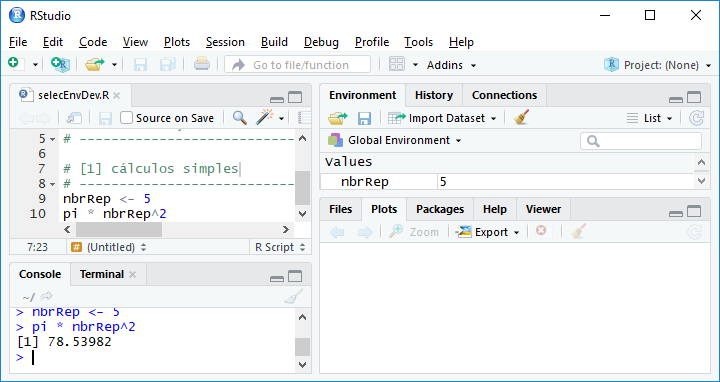
\includegraphics{myFigures/screencap_RStudio_02.png}
\caption{\label{fig:screenCapRStudio02}Capture d'écran de RStudio sous
Windows : exécuter un script avec CTRL +
ENTER.\label{fig:screenCapRStudio02}}
\end{figure}

Nous pouvons voir que par défaut dans la partie du script les
commentaires apparaissent en vert, les chiffres en bleu, et le reste du
code en noir. Dans la partie de la console ce qui a été exécuté apparaît
en bleu et les résultats de l'exécution en noir. Nous pouvons également
noter que dans la partie du code chaque ligne comporte un numéro
correspondant au numéro de ligne à gauche sur fond gris. Il s'agit de la
coloration syntaxique par défaut avec RStudio. Cette coloration
syntaxique peut être modifiée en se rendant dans le menu \emph{Tools},
\emph{Global Options\ldots{}}, \emph{Appearance}, puis en choisissant un
autre thème dans la liste \emph{Editor theme:}. Nous allons choisir le
thème \emph{Cobalt}, puis \emph{OK} (Figure
\ref{fig:screenCapRStudio03}).

\begin{figure}
\centering
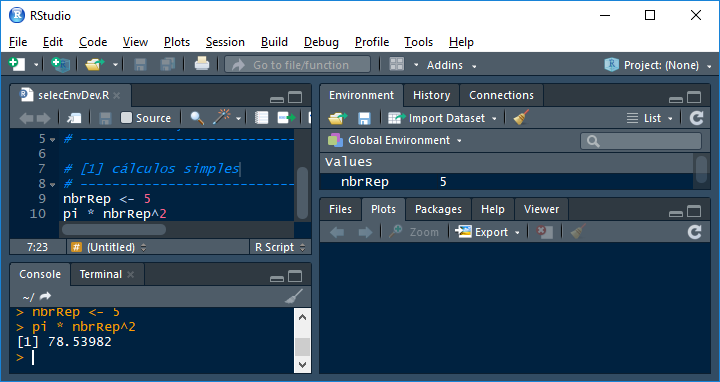
\includegraphics{myFigures/screencap_RStudio_03.png}
\caption{\label{fig:screenCapRStudio03}Capture d'écran de RStudio sous
Windows : changer les paramètres de coloration
syntaxique.\label{fig:screenCapRStudio03}}
\end{figure}

Nous savons comment créer un nouveau script, le sauvegarder, exécuter
son contenu, et changer l'apparence de RStudio. Nous verrons les
nombreux autres avantages de RStudio tout au long de ce livre car c'est
l'environnement de développement qui sera utilisé. Nous serons néanmois
particulièrement vigilents à ce que tous les scripts développés tout au
long de ce livre s'exécute de la même façon quel que soit
l'environnement de développement utilisé.

\section{Notepad++ avec Npp2R}\label{notepad-avec-npp2r}

\begin{figure}
\centering

\includegraphics{myLogos/Notepadpp.png}
\caption{\label{fig:logoNotepad}Logo Notepad++\label{fig:logoNotepad}}
\end{figure}

\subsection{Installer Notepad++ (pour Windows
uniquement)}\label{installer-notepad-pour-windows-uniquement}

Le programme pour installer Notepad++ se trouve dans l'onglet
\emph{Downloads} (\url{https://notepad-plus-plus.org/download/}). Vous
pouvez choisir entre la version 32-bit et 64-bit (64-bit si vous ne
savez pas quelle version choisir). Notepad++ seul est suffisant pour
écrire un script, mais il est encore plus puissant avec \emph{Notepad to
R} (\emph{Npp2R}) qui permet d'exécuter automatiquement nos script dans
une console en local sur notre ordinateur ou à distance sur un serveur.

\subsection{Installer Npp2R}\label{installer-npp2r}

Le programme pour installer Npp2R est hébergé sur le site de Sourceforge
(\url{https://sourceforge.net/projects/npptor/}). Npp2R doit être
installé après Notepad++.

\subsection{Un script avec Notepad++}\label{un-script-avec-notepad}

Lors de la première ouverture Notepad++ affiche un fichier vide
\emph{new 1} (Figura \ref{fig:screenCapNpp01}).

\begin{figure}
\centering
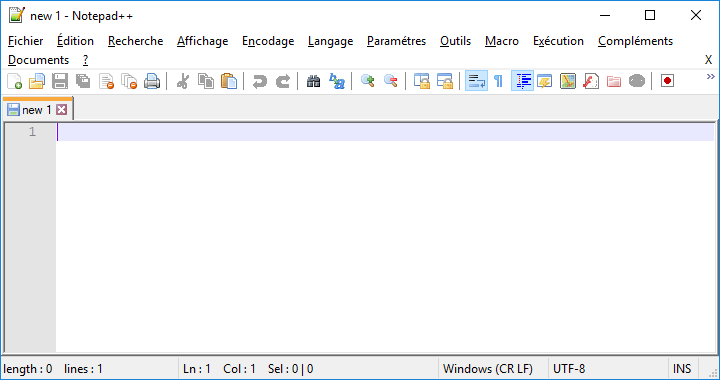
\includegraphics{myFigures/screencap_Npp_01.png}
\caption{\label{fig:screenCapNpp01}Capture d'écran de Notepad++ sous Windows
: fenêtre par défaut.\label{fig:screenCapNpp01}}
\end{figure}

Puisque nous avons déjà créer un script pour le tester avec RStudio,
nous allons l'ouvrir à nouveau avec Notepad++. Dans \emph{Fichier},
selectionnons \emph{Ouvrir\ldots{}} puis choisir le script
\emph{selecEnvDev.R} créé précédemment. Une fois le script ouvert,
allons dans \emph{Langage}, puis \emph{R}, et encore une fois \emph{R}.
La coloration syntaxique apparaît (Figura \ref{fig:screenCapNpp02}).

\begin{figure}
\centering
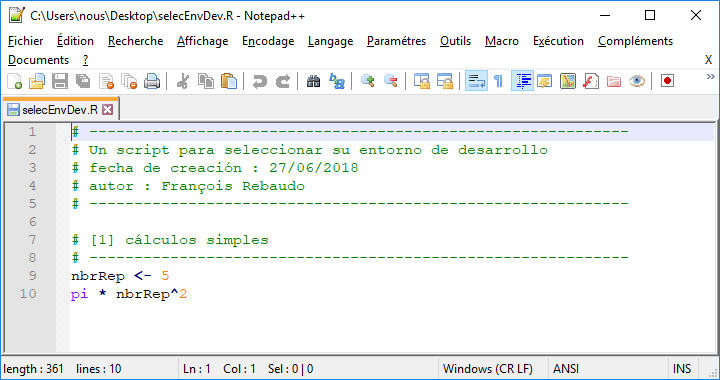
\includegraphics{myFigures/screencap_Npp_02.png}
\caption{\label{fig:screenCapNpp02}Capture d'écran de Notepad++ sous Windows
: exécuter un script avec F8.\label{fig:screenCapNpp02}}
\end{figure}

L'execution du script ne peut se faire que si Npp2R est en cours
d'exécution. Pour se faire il est nécessaire de lancer le programme
Npp2R depuis l'invite de Windows. Un icône devrait apparaître en bas de
votre écran. L'exécution automatique du code depuis Notepad++ se fait en
sélectionnant le code à exécuter puis en utilisant la commande
\texttt{F8}. Si la commande ne fonctionne pas et que vous venez
d'installer Notepad++, il est peut être nécessaire de redémarrer votre
ordinateur. Si la commande fonctionne, une nouvelle fenêtre va s'ouvrir
avec une consol exécutant les lignes souhaitées (Figura
\ref{fig:screenCapNpp03}.

\begin{figure}
\centering
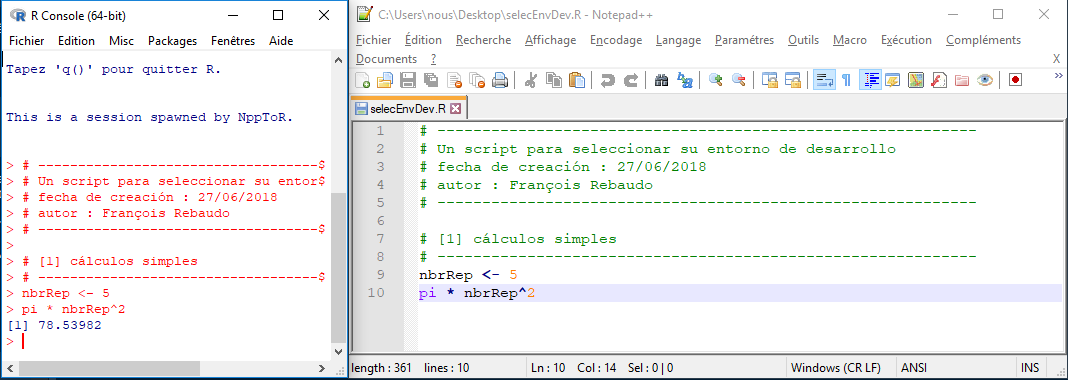
\includegraphics{myFigures/screencap_Npp_03.png}
\caption{\label{fig:screenCapNpp03}Capture d'écran de Notepad++ sous Windows
: la console avec F8.\label{fig:screenCapNpp03}}
\end{figure}

Comme pour RStudio, la coloration syntaxique peut être modifiée depuis
le menu \emph{Paramètres}, et un nouveau thème peut être sélectionné
(par exemple \emph{Solarized} dans la Figura \ref{fig:screenCapNpp04})

\begin{figure}
\centering
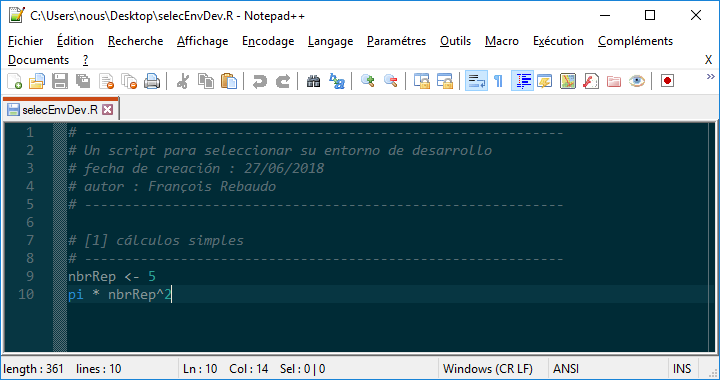
\includegraphics{myFigures/screencap_Npp_04.png}
\caption{\label{fig:screenCapNpp04}Capture d'écran de Notepad++ sous Windows
: coloration syntaxique avec le thème
Solarized.\label{fig:screenCapNpp04}}
\end{figure}

Par rapport aux autres éditeurs de texte, Notepad++ a l'avantage d'être
très léger et offre une vaste gamme d'options pour personnaliser
l'écriture du code.

\section{Geany (pour Linux, Mac OSX et
Windows)}\label{geany-pour-linux-mac-osx-et-windows}

\begin{figure}
\centering

\includegraphics{myLogos/Geany.png}
\caption{\label{fig:logoGeany}Logo Geany\label{fig:logoGeany}}
\end{figure}

\subsection{Installer Geany}\label{installer-geany}

Le programme pour l'installation de Geany se trouve sous l'onglet
\emph{Downloads} dans le menu de gauche \emph{Releases} de la page web
(\url{https://www.geany.org/}). Ensuite il suffit de télécharger
l'exécutable pour Windows ou le dmg pour Mac OSX. Les utilisateurs de
Linux préfèrerons un \texttt{sudo\ apt-get\ install\ geany}.

\subsection{Un script avec Geany}\label{un-script-avec-geany}

Lors de la première ouverture, comme pour RStudio et Notepad++, un
fichier vide est créé (Figure \ref{fig:screenCapGeany01}).

\begin{figure}
\centering
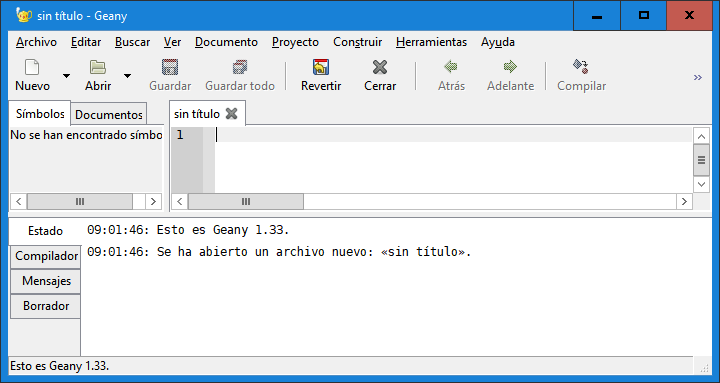
\includegraphics{myFigures/screencap_Geany_01.png}
\caption{\label{fig:screenCapGeany01}Capture d'écran de Geany sous Windows :
fenêtre par défaut.\label{fig:screenCapGeany01}}
\end{figure}

Nous pouvons ouvrir notre script avec \emph{Fichier}, \emph{Ouvrir}
(Figure \ref{fig:screenCapGeany02}).

\begin{figure}
\centering
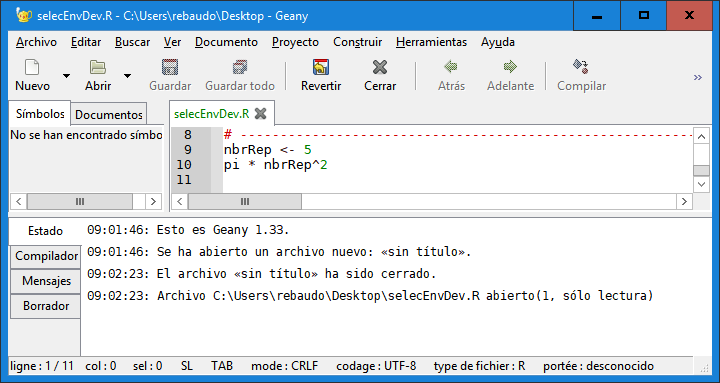
\includegraphics{myFigures/screencap_Geany_02.png}
\caption{\label{fig:screenCapGeany02}Capture d'écran de Geany sous Windows :
ouvrir un script.\label{fig:screenCapGeany02}}
\end{figure}

Pour exécuter notre script, la version de Geany pour Windows ne dispose
pas d'un terminal intégré, ce qui rend son utilisation limitée sous ce
système d'exploitation. L'exécution d'un script peut se faire en ouvrant
R dans une fenêtre à part et en copiant et collant les lignes à
exécuter. Sous Linux et Mac OSX, il suffit d'ouvrir R dans le terminal
situé dans la partie basse de la fenêtre de Geany avec la commande
\texttt{R}. Nous pouvons ensuite paramétré Geany pour qu'une combinaison
de touches permette d'exécuter le code selectionné (par exemple
\texttt{CTRL\ +\ R}). Pour cela il faut tout d'abord autoriser l'envoi
de sélection vers le terminal (\texttt{send\_selection\_unsafe=true})
dans le fichier \texttt{geany.conf} puis choisir la commande d'envoi
vers le terminal (dans \emph{Editar}, \emph{Preferencias},
\emph{Combinaciones}). Pour changer le thème de Geany, il existe une
collection de thèmes accessibles sur GitHub
(\url{https://github.com/geany/geany-themes/}). Le thème peut ensuite
être changé via le menu \emph{Ver}, \emph{Cambiar esquema de
color\ldots{}} (un exemple avec le thème \emph{Solarized}, Figure
\ref{fig:screenCapGeany03}).

\begin{figure}
\centering
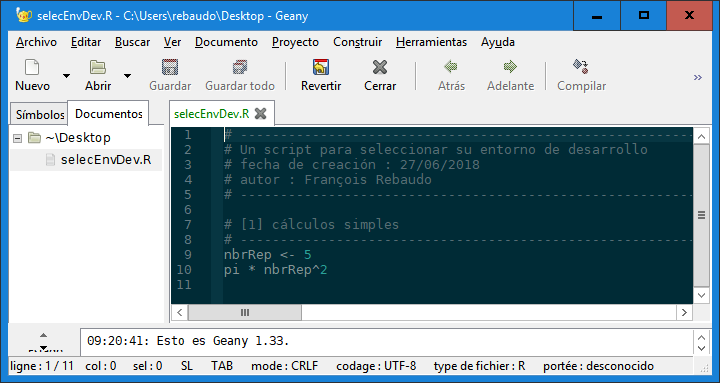
\includegraphics{myFigures/screencap_Geany_03.png}
\caption{\label{fig:screenCapGeany03}Capture d'écran de Geany sous Windows :
changer les paramètres de coloration
syntaxique.\label{fig:screenCapGeany03}}
\end{figure}

\section{Autres solutions}\label{autres-solutions}

Il existe beaucoup d'autres solutions, certaines spécialisées pour R
comme \textbf{Tinn-R} (\url{https://sourceforge.net/projects/tinn-r/}),
et d'autres plus généralistes pour la programmation comme \textbf{Atom}
(\url{https://atom.io/}), \textbf{Sublime Text}
(\url{https://www.sublimetext.com/}), \textbf{Vim}
(\url{https://www.vim.org/}), \textbf{Gedit}
(\url{https://wiki.gnome.org/Apps/Gedit}), \textbf{GNU Emacs}
(\url{https://www.gnu.org/software/emacs/}), ou encore \textbf{Brackets}
(\url{http://brackets.io/}) et \textbf{Eclipse}
(\url{http://www.eclipse.org/}).

\section{Conclusion}\label{conclusion}

Felicitations, nous sommes arrivés au bout de ce chapitre sur
environnements de développement pour utiliser R. Nous savons désormais :

\begin{itemize}
\tightlist
\item
  Installer RStudio, Geany ou Notepad++
\item
  Reconnaître et choisir notre environnement préféré
\end{itemize}

A partir d'ici nous allons pouvoir nous concentrer sur le language de
programmation R dans un environnement facilitant le travail de lecture
et d'écriture du code. C'est un grand pas en avant pour maîtriser R.

\chapter{Les types de données}\label{dataType1}

Nous avons vu précédement comment créer un objet. Un objet est comme une
boîte dans laquelle nous allons \emph{stocker} de l'information. Jusqu'à
présent nous n'avons stocké que des nombres mais dans ce chapitre nous
allons voir qu'il est possible de stocker d'autres informations et nous
allons nous attarder sur les types les plus courants. Dans ce chapitre
nous allons utiliser des \textbf{fonctions} sur lesquelles nous
reviendrons plus tard.

\section{\texorpdfstring{Le type
\texttt{numeric}}{Le type numeric}}\label{le-type-numeric}

Le type \texttt{numeric} correspond à ce que nous avons fait jusqu'à
présent, stocker des nombres. Il existe deux principaux types de nombres
avec R: les nombres entiers (\emph{integers}), et les nombres à virgule
(\emph{double}). Par défaut R considère tous les nombres comme des
nombres à virgule et attribue le type \texttt{double}. Pour vérifier le
type de données nous allons utiliser la fonction \texttt{typeof()} qui
prend comme argument un objet (ou directement l'information que nous
souhaitons tester). Nous pouvons également utiliser la fonction
\texttt{is.double()} qui va renvoyer \texttt{TRUE} si le nombre est au
format \texttt{double} et \texttt{FALSE} dans le cas contraire. La
fonction générique \texttt{is.numeric()} va quant à elle renvoyer
\texttt{TRUE} si l'objet est au format \texttt{numeric} et
\texttt{FALSE} dans le cas contraire.

\begin{Shaded}
\begin{Highlighting}[]
\NormalTok{nbrRep <-}\StringTok{ }\DecValTok{5}
\KeywordTok{typeof}\NormalTok{(nbrRep)}
\end{Highlighting}
\end{Shaded}

\begin{verbatim}
## [1] "double"
\end{verbatim}

\begin{Shaded}
\begin{Highlighting}[]
\KeywordTok{typeof}\NormalTok{(}\FloatTok{5.32}\NormalTok{)}
\end{Highlighting}
\end{Shaded}

\begin{verbatim}
## [1] "double"
\end{verbatim}

\begin{Shaded}
\begin{Highlighting}[]
\KeywordTok{is.numeric}\NormalTok{(}\DecValTok{5}\NormalTok{)}
\end{Highlighting}
\end{Shaded}

\begin{verbatim}
## [1] TRUE
\end{verbatim}

\begin{Shaded}
\begin{Highlighting}[]
\KeywordTok{is.double}\NormalTok{(}\DecValTok{5}\NormalTok{)}
\end{Highlighting}
\end{Shaded}

\begin{verbatim}
## [1] TRUE
\end{verbatim}

Si nous voulons spécifier à R que nous allons travailler avec un nombre
entier, alors il nous faut transformer notre nombre à virgule en nombre
entier avec la fonction \texttt{as.integer()}. Nous pouvons également
utiliser la fonction \texttt{is.integer()} qui va renvoyer \texttt{TRUE}
si le nombre est au format \texttt{integer} et \texttt{FALSE} dans le
cas contraire.

\begin{Shaded}
\begin{Highlighting}[]
\NormalTok{nbrRep <-}\StringTok{ }\KeywordTok{as.integer}\NormalTok{(}\DecValTok{5}\NormalTok{)}
\KeywordTok{typeof}\NormalTok{(nbrRep)}
\end{Highlighting}
\end{Shaded}

\begin{verbatim}
## [1] "integer"
\end{verbatim}

\begin{Shaded}
\begin{Highlighting}[]
\KeywordTok{typeof}\NormalTok{(}\FloatTok{5.32}\NormalTok{)}
\end{Highlighting}
\end{Shaded}

\begin{verbatim}
## [1] "double"
\end{verbatim}

\begin{Shaded}
\begin{Highlighting}[]
\KeywordTok{typeof}\NormalTok{(}\KeywordTok{as.integer}\NormalTok{(}\FloatTok{5.32}\NormalTok{))}
\end{Highlighting}
\end{Shaded}

\begin{verbatim}
## [1] "integer"
\end{verbatim}

\begin{Shaded}
\begin{Highlighting}[]
\KeywordTok{as.integer}\NormalTok{(}\FloatTok{5.32}\NormalTok{)}
\end{Highlighting}
\end{Shaded}

\begin{verbatim}
## [1] 5
\end{verbatim}

\begin{Shaded}
\begin{Highlighting}[]
\KeywordTok{as.integer}\NormalTok{(}\FloatTok{5.99}\NormalTok{)}
\end{Highlighting}
\end{Shaded}

\begin{verbatim}
## [1] 5
\end{verbatim}

\begin{Shaded}
\begin{Highlighting}[]
\KeywordTok{is.numeric}\NormalTok{(nbrRep)}
\end{Highlighting}
\end{Shaded}

\begin{verbatim}
## [1] TRUE
\end{verbatim}

Nous voyons ici que transformer un nombre comme \texttt{5.99} au format
\texttt{integer} va renvoyer uniquement la partie entière, soit
\texttt{5}.

\begin{Shaded}
\begin{Highlighting}[]
\KeywordTok{is.integer}\NormalTok{(}\DecValTok{5}\NormalTok{)}
\end{Highlighting}
\end{Shaded}

\begin{verbatim}
## [1] FALSE
\end{verbatim}

\begin{Shaded}
\begin{Highlighting}[]
\KeywordTok{is.numeric}\NormalTok{(}\DecValTok{5}\NormalTok{)}
\end{Highlighting}
\end{Shaded}

\begin{verbatim}
## [1] TRUE
\end{verbatim}

\begin{Shaded}
\begin{Highlighting}[]
\KeywordTok{is.integer}\NormalTok{(}\KeywordTok{as.integer}\NormalTok{(}\DecValTok{5}\NormalTok{))}
\end{Highlighting}
\end{Shaded}

\begin{verbatim}
## [1] TRUE
\end{verbatim}

\begin{Shaded}
\begin{Highlighting}[]
\KeywordTok{is.numeric}\NormalTok{(}\KeywordTok{as.integer}\NormalTok{(}\DecValTok{5}\NormalTok{))}
\end{Highlighting}
\end{Shaded}

\begin{verbatim}
## [1] TRUE
\end{verbatim}

La somme d'un nombre entier et d'un nombre à virgule renvoie un nombre à
virgule.

\begin{Shaded}
\begin{Highlighting}[]
\NormalTok{sumIntDou <-}\StringTok{ }\KeywordTok{as.integer}\NormalTok{(}\DecValTok{5}\NormalTok{) }\OperatorTok{+}\StringTok{ }\FloatTok{5.2}
\KeywordTok{typeof}\NormalTok{(sumIntDou)}
\end{Highlighting}
\end{Shaded}

\begin{verbatim}
## [1] "double"
\end{verbatim}

\begin{Shaded}
\begin{Highlighting}[]
\NormalTok{sumIntInt <-}\StringTok{ }\KeywordTok{as.integer}\NormalTok{(}\DecValTok{5}\NormalTok{) }\OperatorTok{+}\StringTok{ }\KeywordTok{as.integer}\NormalTok{(}\DecValTok{5}\NormalTok{)}
\KeywordTok{typeof}\NormalTok{(sumIntInt)}
\end{Highlighting}
\end{Shaded}

\begin{verbatim}
## [1] "integer"
\end{verbatim}

Pour résumer, le type \texttt{numeric} contient deux sous-types, les
types \texttt{intger} pour les nombres entiers et le type
\texttt{double} pour les nombres à virgule. Par défaut R attribue le
type \texttt{double} aux nombres.

\section{\texorpdfstring{Le type
\texttt{character}}{Le type character}}\label{le-type-character}

Le type \texttt{character} correspond au texte. En effet, R permet de
travailler avec du texte. pour spécifier à R que l'information contenue
dans un objet est au format texte (ou de manière générale pour tous les
textes), il faut utiliser les guillemets doubles (\texttt{"}), ou
simples (\texttt{\textquotesingle{}}).

\begin{Shaded}
\begin{Highlighting}[]
\NormalTok{myText <-}\StringTok{ "azerty"}
\NormalTok{myText2 <-}\StringTok{ 'azerty'}
\NormalTok{myText3 <-}\StringTok{ 'azerty uiop qsdfg hjklm'}
\KeywordTok{typeof}\NormalTok{(myText3)}
\end{Highlighting}
\end{Shaded}

\begin{verbatim}
## [1] "character"
\end{verbatim}

Les guillemets doubles ou simples sont utiles si l'on souhaite mettre
des guillemets dans notre texte. Nous pouvons également \emph{échapper}
un caractère spécial comme un guillemet grâce au signe backslash
\texttt{\textbackslash{}}.

\begin{Shaded}
\begin{Highlighting}[]
\NormalTok{myText <-}\StringTok{ "a 'ze' 'rt' y"}
\NormalTok{myText2 <-}\StringTok{ 'a "zert" y'}
\NormalTok{myText3 <-}\StringTok{ 'azerty uiop qsdfg hjklm'}
\NormalTok{myText4 <-}\StringTok{ "qwerty }\CharTok{\textbackslash{}"}\StringTok{ azerty "}
\NormalTok{myText5 <-}\StringTok{ "qwerty }\CharTok{\textbackslash{}\textbackslash{}}\StringTok{ azerty "}
\end{Highlighting}
\end{Shaded}

Par défaut lorsque nous créons un objet, son contenu n'est pas renvoyé
par la console. Sur Internet ou dans de nombreux ouvrages nous pouvons
retrouver le nom de l'objet sur une ligne pour renvoyer son contenu:

\begin{Shaded}
\begin{Highlighting}[]
\NormalTok{myText <-}\StringTok{ "a 'ze' 'rt' y"}
\NormalTok{myText}
\end{Highlighting}
\end{Shaded}

\begin{verbatim}
## [1] "a 'ze' 'rt' y"
\end{verbatim}

Dans ce livre nous n'utiliserons jamais cette façon de faire et
préfèrerons l'utilisation de la fonction \texttt{print()}, qui permet
d'afficher dans la console le contenu d'un objet. Le résultat est le
même mais le code est alors plus facile à lire et plus explicite sur ce
qui est fait.

\begin{Shaded}
\begin{Highlighting}[]
\NormalTok{myText <-}\StringTok{ "a 'ze' 'rt' y"}
\KeywordTok{print}\NormalTok{(myText)}
\end{Highlighting}
\end{Shaded}

\begin{verbatim}
## [1] "a 'ze' 'rt' y"
\end{verbatim}

\begin{Shaded}
\begin{Highlighting}[]
\NormalTok{nbrRep <-}\StringTok{ }\DecValTok{5}
\KeywordTok{print}\NormalTok{(nbrRep)}
\end{Highlighting}
\end{Shaded}

\begin{verbatim}
## [1] 5
\end{verbatim}

Nous pouvons également mettre des chiffres au format texte, mais il ne
faut pas oublier de mettre des guillemets pour spécifier le type
\texttt{character} ou utiliser la fonction \texttt{as.character()}. Une
opération entre du texte et un nombre renvoie une erreur. Par exemple si
l'on ajoute \texttt{10} à \texttt{"5"}, R nous signale qu'un
\textbf{argument} de la \textbf{fonction} \texttt{+} n'est pas de type
\texttt{numeric} et que donc l'opération n'est pas possible. Nous ne
pouvons pas non plus ajouter du texte a du texte, mais verrons plus tard
comment \emph{concaténer} deux \emph{chaines de texte}.

\begin{Shaded}
\begin{Highlighting}[]
\NormalTok{myText <-}\StringTok{ "qwerty"}
\KeywordTok{typeof}\NormalTok{(myText)}
\end{Highlighting}
\end{Shaded}

\begin{verbatim}
## [1] "character"
\end{verbatim}

\begin{Shaded}
\begin{Highlighting}[]
\NormalTok{myText2 <-}\StringTok{ }\DecValTok{5}
\KeywordTok{typeof}\NormalTok{(myText2)}
\end{Highlighting}
\end{Shaded}

\begin{verbatim}
## [1] "double"
\end{verbatim}

\begin{Shaded}
\begin{Highlighting}[]
\NormalTok{myText3 <-}\StringTok{ "5"}
\KeywordTok{typeof}\NormalTok{(myText3)}
\end{Highlighting}
\end{Shaded}

\begin{verbatim}
## [1] "character"
\end{verbatim}

\begin{Shaded}
\begin{Highlighting}[]
\NormalTok{myText2 }\OperatorTok{+}\StringTok{ }\DecValTok{10}
\end{Highlighting}
\end{Shaded}

\begin{verbatim}
## [1] 15
\end{verbatim}

\begin{Shaded}
\begin{Highlighting}[]
\KeywordTok{as.character}\NormalTok{(}\DecValTok{5}\NormalTok{)}
\end{Highlighting}
\end{Shaded}

\begin{verbatim}
## [1] "5"
\end{verbatim}

\begin{Shaded}
\begin{Highlighting}[]
\CommentTok{# myText3 + 10 # Error in myText3 + 10 : non-numeric argument to binary operator}
\CommentTok{# "a" + "b" # Error in "a" + "b" : non-numeric argument to binary operator}
\end{Highlighting}
\end{Shaded}

Pour résumer, le type \texttt{character} permet la saisie de texte, nous
pouvons le reconnaître grâce aux guillemets simples ou doubles.

\section{\texorpdfstring{Le type
\texttt{factor}}{Le type factor}}\label{le-type-factor}

Le type \texttt{factor} correspond aux facteurs. Les facteurs sont un
choix parmi une liste finie de possibilités. Par exemple les pays sont
des facteurs car il y a une liste finie de pays dans le monde à un temps
donné. Un facteur peut être défini avec la fonction \texttt{factor()} ou
transformé en utilisant la fonction \texttt{as.factor()}. Comme pour les
autres types de donnée nous pouvons utiliser la fonction
\texttt{is.factor()} pour vérifier le type de donnée. Pour avoir la
liste de toutes les possibilités, il existe la fonction
\texttt{levels()} (cette fonction prendra plus de sens quand nous aurons
abordé les types de conteneur de l'information).

\begin{Shaded}
\begin{Highlighting}[]
\NormalTok{factor01 <-}\StringTok{ }\KeywordTok{factor}\NormalTok{(}\StringTok{"aaa"}\NormalTok{)}
\KeywordTok{print}\NormalTok{(factor01)}
\end{Highlighting}
\end{Shaded}

\begin{verbatim}
## [1] aaa
## Levels: aaa
\end{verbatim}

\begin{Shaded}
\begin{Highlighting}[]
\KeywordTok{typeof}\NormalTok{(factor01)}
\end{Highlighting}
\end{Shaded}

\begin{verbatim}
## [1] "integer"
\end{verbatim}

\begin{Shaded}
\begin{Highlighting}[]
\KeywordTok{is.factor}\NormalTok{(factor01)}
\end{Highlighting}
\end{Shaded}

\begin{verbatim}
## [1] TRUE
\end{verbatim}

\begin{Shaded}
\begin{Highlighting}[]
\KeywordTok{levels}\NormalTok{(factor01)}
\end{Highlighting}
\end{Shaded}

\begin{verbatim}
## [1] "aaa"
\end{verbatim}

Un facteur peut être transformé en texte avec la fonction
\texttt{as.character()} mais également en nombre avec
\texttt{as.numeric()}. Lors de la transformation en nombre chaque
facteur prend la valeur de sa position dans la liste des possibilités.
Dans notre cas il n'y a qu'une seule possibilité donc la fonction
\texttt{as.numeric()} va renvoyer \texttt{1}:

\begin{Shaded}
\begin{Highlighting}[]
\NormalTok{factor01 <-}\StringTok{ }\KeywordTok{factor}\NormalTok{(}\StringTok{"aaa"}\NormalTok{)}
\KeywordTok{as.character}\NormalTok{(factor01)}
\end{Highlighting}
\end{Shaded}

\begin{verbatim}
## [1] "aaa"
\end{verbatim}

\begin{Shaded}
\begin{Highlighting}[]
\KeywordTok{as.numeric}\NormalTok{(factor01)}
\end{Highlighting}
\end{Shaded}

\begin{verbatim}
## [1] 1
\end{verbatim}

\section{\texorpdfstring{Le type
\texttt{logical}}{Le type logical}}\label{le-type-logical}

Le type \texttt{logical} correspond aux valeurs \texttt{TRUE} et
\texttt{FALSE} (et \texttt{NA}) que nous avons déjà vu avec les
opérateurs de comparaison.

\begin{Shaded}
\begin{Highlighting}[]
\NormalTok{aLogic <-}\StringTok{ }\OtherTok{TRUE}
\KeywordTok{print}\NormalTok{(aLogic)}
\end{Highlighting}
\end{Shaded}

\begin{verbatim}
## [1] TRUE
\end{verbatim}

\begin{Shaded}
\begin{Highlighting}[]
\KeywordTok{typeof}\NormalTok{(aLogic)}
\end{Highlighting}
\end{Shaded}

\begin{verbatim}
## [1] "logical"
\end{verbatim}

\begin{Shaded}
\begin{Highlighting}[]
\KeywordTok{is.logical}\NormalTok{(aLogic)}
\end{Highlighting}
\end{Shaded}

\begin{verbatim}
## [1] TRUE
\end{verbatim}

\begin{Shaded}
\begin{Highlighting}[]
\NormalTok{aLogic }\OperatorTok{+}\StringTok{ }\DecValTok{1}
\end{Highlighting}
\end{Shaded}

\begin{verbatim}
## [1] 2
\end{verbatim}

\begin{Shaded}
\begin{Highlighting}[]
\KeywordTok{as.numeric}\NormalTok{(aLogic)}
\end{Highlighting}
\end{Shaded}

\begin{verbatim}
## [1] 1
\end{verbatim}

\begin{Shaded}
\begin{Highlighting}[]
\KeywordTok{as.character}\NormalTok{(aLogic)}
\end{Highlighting}
\end{Shaded}

\begin{verbatim}
## [1] "TRUE"
\end{verbatim}

\section{\texorpdfstring{A propos de
\texttt{NA}}{A propos de NA}}\label{a-propos-de-na}

La valeur \texttt{NA} peut être utilisée pour spécifier l'absence de
données ou les données manquantes. Par défaut \texttt{NA} est de type
\texttt{logical} mais il peut être utilisé pour du texte, ou des
nombres.

\begin{Shaded}
\begin{Highlighting}[]
\KeywordTok{print}\NormalTok{(}\OtherTok{NA}\NormalTok{)}
\end{Highlighting}
\end{Shaded}

\begin{verbatim}
## [1] NA
\end{verbatim}

\begin{Shaded}
\begin{Highlighting}[]
\KeywordTok{typeof}\NormalTok{(}\OtherTok{NA}\NormalTok{)}
\end{Highlighting}
\end{Shaded}

\begin{verbatim}
## [1] "logical"
\end{verbatim}

\begin{Shaded}
\begin{Highlighting}[]
\KeywordTok{typeof}\NormalTok{(}\KeywordTok{as.integer}\NormalTok{(}\OtherTok{NA}\NormalTok{))}
\end{Highlighting}
\end{Shaded}

\begin{verbatim}
## [1] "integer"
\end{verbatim}

\begin{Shaded}
\begin{Highlighting}[]
\KeywordTok{typeof}\NormalTok{(}\KeywordTok{as.character}\NormalTok{(}\OtherTok{NA}\NormalTok{))}
\end{Highlighting}
\end{Shaded}

\begin{verbatim}
## [1] "character"
\end{verbatim}

\begin{Shaded}
\begin{Highlighting}[]
\OtherTok{NA} \OperatorTok{==}\StringTok{ }\OtherTok{TRUE}
\end{Highlighting}
\end{Shaded}

\begin{verbatim}
## [1] NA
\end{verbatim}

\begin{Shaded}
\begin{Highlighting}[]
\OtherTok{NA} \OperatorTok{==}\StringTok{ }\OtherTok{FALSE}
\end{Highlighting}
\end{Shaded}

\begin{verbatim}
## [1] NA
\end{verbatim}

\begin{Shaded}
\begin{Highlighting}[]
\OtherTok{NA} \OperatorTok{>}\StringTok{ }\DecValTok{1}
\end{Highlighting}
\end{Shaded}

\begin{verbatim}
## [1] NA
\end{verbatim}

\begin{Shaded}
\begin{Highlighting}[]
\OtherTok{NA} \OperatorTok{+}\StringTok{ }\DecValTok{1}
\end{Highlighting}
\end{Shaded}

\begin{verbatim}
## [1] NA
\end{verbatim}

\section{Conclusion}\label{conclusion-1}

Felicitations, nous sommes arrivés au bout de ce chapitre sur les type
de données. Nous savons désormais :

\begin{itemize}
\tightlist
\item
  Reconnaîte et faire des objets dans les principaux types de données
\item
  Transformer les types de données d'un type à un autre
\end{itemize}

Ce chapitre un peu fastidieux est la base pour aborder le prochain
chapitre sur les conteneurs des données.

\chapter{Les conteneurs de données}\label{dataType2}

Jusqu'à présent nous avons fait des objets simples ne contenant qu'une
seule valeur. Nous avons néanmoins pu voir qu'un objet avait différents
attributs, comme sa valeur, mais aussi le type de donnée contenue.
maintenant nous allons voir qu'il existe différents types de conteneurs
permettant de stocker plusieurs données.

\section{\texorpdfstring{Le conteneur
\texttt{vector}}{Le conteneur vector}}\label{le-conteneur-vector}

Dans R, un \texttt{vector} est une combinaison de données avec la
particularité que toutes les données contenues dans un \texttt{vector}
sont du même type. Nous pouvons donc stocker plusieurs \texttt{numeric}
ou \texttt{character} dans un \texttt{vector}, mais pas les deux. Le
conteneur \texttt{vector} est important car c'est l'élément de base de
R.

\subsection{\texorpdfstring{Créer un
\texttt{vector}}{Créer un vector}}\label{creer-un-vector}

Pour créer un \texttt{vector} nous allons utiliser la fonction
\texttt{c()} qui permet de combiner des éléments en un \texttt{vector}.
Les éléments à combiner doivent être séparés par des virgules.

\begin{Shaded}
\begin{Highlighting}[]
\NormalTok{miVec01 <-}\StringTok{ }\KeywordTok{c}\NormalTok{(}\DecValTok{1}\NormalTok{, }\DecValTok{2}\NormalTok{, }\DecValTok{3}\NormalTok{, }\DecValTok{4}\NormalTok{) }\CommentTok{# un vecteur de 4 éléments de type numeric ; double}
\KeywordTok{print}\NormalTok{(miVec01)}
\end{Highlighting}
\end{Shaded}

\begin{verbatim}
## [1] 1 2 3 4
\end{verbatim}

\begin{Shaded}
\begin{Highlighting}[]
\KeywordTok{typeof}\NormalTok{(miVec01)}
\end{Highlighting}
\end{Shaded}

\begin{verbatim}
## [1] "double"
\end{verbatim}

\begin{Shaded}
\begin{Highlighting}[]
\KeywordTok{is.vector}\NormalTok{(miVec01)}
\end{Highlighting}
\end{Shaded}

\begin{verbatim}
## [1] TRUE
\end{verbatim}

La fonction \texttt{is.vector()} permet de vérifier le type de
conteneur.

\begin{Shaded}
\begin{Highlighting}[]
\NormalTok{miVec02 <-}\StringTok{ }\KeywordTok{c}\NormalTok{(}\StringTok{"a"}\NormalTok{, }\StringTok{"b"}\NormalTok{, }\StringTok{"c"}\NormalTok{) }
\KeywordTok{print}\NormalTok{(miVec02)}
\end{Highlighting}
\end{Shaded}

\begin{verbatim}
## [1] "a" "b" "c"
\end{verbatim}

\begin{Shaded}
\begin{Highlighting}[]
\KeywordTok{typeof}\NormalTok{(miVec02)}
\end{Highlighting}
\end{Shaded}

\begin{verbatim}
## [1] "character"
\end{verbatim}

\begin{Shaded}
\begin{Highlighting}[]
\KeywordTok{is.vector}\NormalTok{(miVec02)}
\end{Highlighting}
\end{Shaded}

\begin{verbatim}
## [1] TRUE
\end{verbatim}

\begin{Shaded}
\begin{Highlighting}[]
\NormalTok{miVec03 <-}\StringTok{ }\KeywordTok{c}\NormalTok{(}\OtherTok{TRUE}\NormalTok{, }\OtherTok{FALSE}\NormalTok{, }\OtherTok{FALSE}\NormalTok{, }\OtherTok{TRUE}\NormalTok{)}
\KeywordTok{print}\NormalTok{(miVec03)}
\end{Highlighting}
\end{Shaded}

\begin{verbatim}
## [1]  TRUE FALSE FALSE  TRUE
\end{verbatim}

\begin{Shaded}
\begin{Highlighting}[]
\KeywordTok{typeof}\NormalTok{(miVec03)}
\end{Highlighting}
\end{Shaded}

\begin{verbatim}
## [1] "logical"
\end{verbatim}

\begin{Shaded}
\begin{Highlighting}[]
\KeywordTok{is.vector}\NormalTok{(miVec03)}
\end{Highlighting}
\end{Shaded}

\begin{verbatim}
## [1] TRUE
\end{verbatim}

\begin{Shaded}
\begin{Highlighting}[]
\NormalTok{miVecNA <-}\StringTok{ }\KeywordTok{c}\NormalTok{(}\DecValTok{1}\NormalTok{, }\OtherTok{NA}\NormalTok{, }\DecValTok{3}\NormalTok{, }\OtherTok{NA}\NormalTok{, }\DecValTok{5}\NormalTok{)}
\KeywordTok{print}\NormalTok{(miVecNA)}
\end{Highlighting}
\end{Shaded}

\begin{verbatim}
## [1]  1 NA  3 NA  5
\end{verbatim}

\begin{Shaded}
\begin{Highlighting}[]
\KeywordTok{typeof}\NormalTok{(miVecNA)}
\end{Highlighting}
\end{Shaded}

\begin{verbatim}
## [1] "double"
\end{verbatim}

\begin{Shaded}
\begin{Highlighting}[]
\KeywordTok{is.vector}\NormalTok{(miVecNA)}
\end{Highlighting}
\end{Shaded}

\begin{verbatim}
## [1] TRUE
\end{verbatim}

\begin{Shaded}
\begin{Highlighting}[]
\NormalTok{miVec04 <-}\StringTok{ }\KeywordTok{c}\NormalTok{(}\DecValTok{1}\NormalTok{, }\StringTok{"a"}\NormalTok{)}
\KeywordTok{print}\NormalTok{(miVec04)}
\end{Highlighting}
\end{Shaded}

\begin{verbatim}
## [1] "1" "a"
\end{verbatim}

\begin{Shaded}
\begin{Highlighting}[]
\KeywordTok{typeof}\NormalTok{(miVec04)}
\end{Highlighting}
\end{Shaded}

\begin{verbatim}
## [1] "character"
\end{verbatim}

\begin{Shaded}
\begin{Highlighting}[]
\KeywordTok{is.vector}\NormalTok{(miVec04)}
\end{Highlighting}
\end{Shaded}

\begin{verbatim}
## [1] TRUE
\end{verbatim}

Si l'on combine différents types de données, par défaut R va chercher à
transformer les éléments en un seul type. Si comme ici dans l'objet
\texttt{miVec03} nous avons des \texttt{character} et des
\texttt{numeric}, R va transformer tous les éléments en
\texttt{character}.

\begin{Shaded}
\begin{Highlighting}[]
\NormalTok{miVec05 <-}\StringTok{ }\KeywordTok{c}\NormalTok{(}\KeywordTok{factor}\NormalTok{(}\StringTok{"abc"}\NormalTok{), }\StringTok{"def"}\NormalTok{)}
\KeywordTok{print}\NormalTok{(miVec05)}
\end{Highlighting}
\end{Shaded}

\begin{verbatim}
## [1] "1"   "def"
\end{verbatim}

\begin{Shaded}
\begin{Highlighting}[]
\KeywordTok{typeof}\NormalTok{(miVec05)}
\end{Highlighting}
\end{Shaded}

\begin{verbatim}
## [1] "character"
\end{verbatim}

\begin{Shaded}
\begin{Highlighting}[]
\NormalTok{miVec06 <-}\StringTok{ }\KeywordTok{c}\NormalTok{(}\OtherTok{TRUE}\NormalTok{, }\StringTok{"def"}\NormalTok{)}
\KeywordTok{print}\NormalTok{(miVec06)}
\end{Highlighting}
\end{Shaded}

\begin{verbatim}
## [1] "TRUE" "def"
\end{verbatim}

\begin{Shaded}
\begin{Highlighting}[]
\KeywordTok{typeof}\NormalTok{(miVec06)}
\end{Highlighting}
\end{Shaded}

\begin{verbatim}
## [1] "character"
\end{verbatim}

\begin{Shaded}
\begin{Highlighting}[]
\NormalTok{miVec07 <-}\StringTok{ }\KeywordTok{c}\NormalTok{(}\KeywordTok{factor}\NormalTok{(}\StringTok{"abc"}\NormalTok{), }\DecValTok{55}\NormalTok{)}
\KeywordTok{print}\NormalTok{(miVec07)}
\end{Highlighting}
\end{Shaded}

\begin{verbatim}
## [1]  1 55
\end{verbatim}

\begin{Shaded}
\begin{Highlighting}[]
\KeywordTok{typeof}\NormalTok{(miVec07)}
\end{Highlighting}
\end{Shaded}

\begin{verbatim}
## [1] "double"
\end{verbatim}

\begin{Shaded}
\begin{Highlighting}[]
\NormalTok{miVec08 <-}\StringTok{ }\KeywordTok{c}\NormalTok{(}\OtherTok{TRUE}\NormalTok{, }\DecValTok{55}\NormalTok{)}
\KeywordTok{print}\NormalTok{(miVec08)}
\end{Highlighting}
\end{Shaded}

\begin{verbatim}
## [1]  1 55
\end{verbatim}

\begin{Shaded}
\begin{Highlighting}[]
\KeywordTok{typeof}\NormalTok{(miVec08)}
\end{Highlighting}
\end{Shaded}

\begin{verbatim}
## [1] "double"
\end{verbatim}

Nous pouvons aussi combiner des objets existants au sein d'un
\texttt{vector}.

\begin{Shaded}
\begin{Highlighting}[]
\NormalTok{miVec09 <-}\StringTok{ }\KeywordTok{c}\NormalTok{(miVec02, }\StringTok{"d"}\NormalTok{, }\StringTok{"e"}\NormalTok{, }\StringTok{"f"}\NormalTok{)}
\KeywordTok{print}\NormalTok{(miVec09)}
\end{Highlighting}
\end{Shaded}

\begin{verbatim}
## [1] "a" "b" "c" "d" "e" "f"
\end{verbatim}

\begin{Shaded}
\begin{Highlighting}[]
\NormalTok{miVec10 <-}\StringTok{ }\KeywordTok{c}\NormalTok{(}\StringTok{"aaa"}\NormalTok{, }\StringTok{"aa"}\NormalTok{, miVec09, }\StringTok{"d"}\NormalTok{, }\StringTok{"e"}\NormalTok{, }\StringTok{"f"}\NormalTok{)}
\KeywordTok{print}\NormalTok{(miVec10)}
\end{Highlighting}
\end{Shaded}

\begin{verbatim}
##  [1] "aaa" "aa"  "a"   "b"   "c"   "d"   "e"   "f"   "d"   "e"   "f"
\end{verbatim}

\begin{Shaded}
\begin{Highlighting}[]
\NormalTok{miVec11 <-}\StringTok{ }\KeywordTok{c}\NormalTok{(}\DecValTok{789}\NormalTok{, miVec01 , }\DecValTok{564}\NormalTok{)}
\KeywordTok{print}\NormalTok{(miVec11)}
\end{Highlighting}
\end{Shaded}

\begin{verbatim}
## [1] 789   1   2   3   4 564
\end{verbatim}

\subsection{\texorpdfstring{Opérations sur un
\texttt{vector}}{Opérations sur un vector}}\label{operations-sur-un-vector}

Nous pouvons également effectuer des opération sur un \texttt{vector}.

\begin{Shaded}
\begin{Highlighting}[]
\KeywordTok{print}\NormalTok{(miVec01)}
\end{Highlighting}
\end{Shaded}

\begin{verbatim}
## [1] 1 2 3 4
\end{verbatim}

\begin{Shaded}
\begin{Highlighting}[]
\NormalTok{miVec01 }\OperatorTok{+}\StringTok{ }\DecValTok{1}
\end{Highlighting}
\end{Shaded}

\begin{verbatim}
## [1] 2 3 4 5
\end{verbatim}

\begin{Shaded}
\begin{Highlighting}[]
\NormalTok{miVec01 }\OperatorTok{-}\StringTok{ }\DecValTok{1}
\end{Highlighting}
\end{Shaded}

\begin{verbatim}
## [1] 0 1 2 3
\end{verbatim}

\begin{Shaded}
\begin{Highlighting}[]
\NormalTok{miVec01 }\OperatorTok{*}\StringTok{ }\DecValTok{2}
\end{Highlighting}
\end{Shaded}

\begin{verbatim}
## [1] 2 4 6 8
\end{verbatim}

\begin{Shaded}
\begin{Highlighting}[]
\NormalTok{miVec01 }\OperatorTok{/}\DecValTok{10}
\end{Highlighting}
\end{Shaded}

\begin{verbatim}
## [1] 0.1 0.2 0.3 0.4
\end{verbatim}

Les opérations d'un \texttt{vector} sur un autre sont aussi possibles,
mais il faut veiller à ce que le nombre d'éléments d'un \texttt{vector}
soit le même que l'autre, sinon R va effectuer le calcul en repartant du
début. Voici un exemple pour illustrer ce que R fait:

\begin{Shaded}
\begin{Highlighting}[]
\NormalTok{miVec12 <-}\StringTok{ }\KeywordTok{c}\NormalTok{(}\DecValTok{1}\NormalTok{, }\DecValTok{1}\NormalTok{, }\DecValTok{1}\NormalTok{, }\DecValTok{1}\NormalTok{, }\DecValTok{1}\NormalTok{, }\DecValTok{1}\NormalTok{, }\DecValTok{1}\NormalTok{, }\DecValTok{1}\NormalTok{, }\DecValTok{1}\NormalTok{)}
\KeywordTok{print}\NormalTok{(miVec12)}
\end{Highlighting}
\end{Shaded}

\begin{verbatim}
## [1] 1 1 1 1 1 1 1 1 1
\end{verbatim}

\begin{Shaded}
\begin{Highlighting}[]
\NormalTok{miVec13 <-}\StringTok{ }\KeywordTok{c}\NormalTok{(}\DecValTok{10}\NormalTok{, }\DecValTok{20}\NormalTok{, }\DecValTok{30}\NormalTok{)}
\KeywordTok{print}\NormalTok{(miVec13)}
\end{Highlighting}
\end{Shaded}

\begin{verbatim}
## [1] 10 20 30
\end{verbatim}

\begin{Shaded}
\begin{Highlighting}[]
\NormalTok{miVec12 }\OperatorTok{+}\StringTok{ }\NormalTok{miVec13 }\CommentTok{# vecteurs de tailles différentes : attention au résultat}
\end{Highlighting}
\end{Shaded}

\begin{verbatim}
## [1] 11 21 31 11 21 31 11 21 31
\end{verbatim}

\begin{Shaded}
\begin{Highlighting}[]
\NormalTok{miVec14 <-}\StringTok{ }\KeywordTok{c}\NormalTok{(}\DecValTok{10}\NormalTok{, }\DecValTok{20}\NormalTok{, }\DecValTok{30}\NormalTok{, }\DecValTok{40}\NormalTok{, }\DecValTok{50}\NormalTok{, }\DecValTok{60}\NormalTok{, }\DecValTok{70}\NormalTok{, }\DecValTok{80}\NormalTok{, }\DecValTok{90}\NormalTok{)}
\KeywordTok{print}\NormalTok{(miVec14)}
\end{Highlighting}
\end{Shaded}

\begin{verbatim}
## [1] 10 20 30 40 50 60 70 80 90
\end{verbatim}

\begin{Shaded}
\begin{Highlighting}[]
\NormalTok{miVec12 }\OperatorTok{+}\StringTok{ }\NormalTok{miVec14 }\CommentTok{# les vecteurs sont de la même longueur}
\end{Highlighting}
\end{Shaded}

\begin{verbatim}
## [1] 11 21 31 41 51 61 71 81 91
\end{verbatim}

\begin{Shaded}
\begin{Highlighting}[]
\NormalTok{miVec15 <-}\StringTok{ }\KeywordTok{c}\NormalTok{(}\DecValTok{1}\NormalTok{, }\DecValTok{1}\NormalTok{, }\DecValTok{1}\NormalTok{, }\DecValTok{1}\NormalTok{)}
\KeywordTok{print}\NormalTok{(miVec15)}
\end{Highlighting}
\end{Shaded}

\begin{verbatim}
## [1] 1 1 1 1
\end{verbatim}

\begin{Shaded}
\begin{Highlighting}[]
\NormalTok{miVec15 }\OperatorTok{+}\StringTok{ }\NormalTok{miVec13 }\CommentTok{# vecteurs de tailles différentes et non multiples}
\end{Highlighting}
\end{Shaded}

\begin{verbatim}
## Warning in miVec15 + miVec13: la taille d'un objet plus long n'est pas
## multiple de la taille d'un objet plus court
\end{verbatim}

\begin{verbatim}
## [1] 11 21 31 11
\end{verbatim}

\subsection{\texorpdfstring{Accèder aux valeurs d'un
\texttt{vector}}{Accèder aux valeurs d'un vector}}\label{acceder-aux-valeurs-dun-vector}

Il souvent nécessaire de pouvoir accèder aux valeurs d'un
\texttt{vector}, c'est à dire de récupérer une valeur ou un groupe de
valeurs au sein d'un \texttt{vector}. Pour à un élément dans un
\texttt{vector} nous utilisons les crochets \texttt{{[}{]}}. Entre les
crochets, nous pouvons utiliser un numéro correspondant au numéro de
l'élément dans le \texttt{vector}.

\begin{Shaded}
\begin{Highlighting}[]
\NormalTok{miVec20 <-}\StringTok{ }\KeywordTok{c}\NormalTok{(}\DecValTok{10}\NormalTok{, }\DecValTok{20}\NormalTok{, }\DecValTok{30}\NormalTok{, }\DecValTok{40}\NormalTok{, }\DecValTok{50}\NormalTok{, }\DecValTok{60}\NormalTok{, }\DecValTok{70}\NormalTok{, }\DecValTok{80}\NormalTok{, }\DecValTok{90}\NormalTok{)}
\NormalTok{miVec21 <-}\StringTok{ }\KeywordTok{c}\NormalTok{(}\StringTok{"a"}\NormalTok{, }\StringTok{"b"}\NormalTok{, }\StringTok{"c"}\NormalTok{, }\StringTok{"d"}\NormalTok{, }\StringTok{"e"}\NormalTok{, }\StringTok{"f"}\NormalTok{, }\StringTok{"g"}\NormalTok{, }\StringTok{"h"}\NormalTok{, }\StringTok{"i"}\NormalTok{)}
\KeywordTok{print}\NormalTok{(miVec20)}
\end{Highlighting}
\end{Shaded}

\begin{verbatim}
## [1] 10 20 30 40 50 60 70 80 90
\end{verbatim}

\begin{Shaded}
\begin{Highlighting}[]
\KeywordTok{print}\NormalTok{(miVec21)}
\end{Highlighting}
\end{Shaded}

\begin{verbatim}
## [1] "a" "b" "c" "d" "e" "f" "g" "h" "i"
\end{verbatim}

\begin{Shaded}
\begin{Highlighting}[]
\KeywordTok{print}\NormalTok{(miVec20[}\DecValTok{1}\NormalTok{])}
\end{Highlighting}
\end{Shaded}

\begin{verbatim}
## [1] 10
\end{verbatim}

\begin{Shaded}
\begin{Highlighting}[]
\KeywordTok{print}\NormalTok{(miVec21[}\DecValTok{3}\NormalTok{])}
\end{Highlighting}
\end{Shaded}

\begin{verbatim}
## [1] "c"
\end{verbatim}

Nous pouvons aussi utiliser la combinaison de différents éléments (un
autre \texttt{vector}).

\begin{Shaded}
\begin{Highlighting}[]
\KeywordTok{print}\NormalTok{(miVec20[}\KeywordTok{c}\NormalTok{(}\DecValTok{1}\NormalTok{, }\DecValTok{5}\NormalTok{, }\DecValTok{9}\NormalTok{)])}
\end{Highlighting}
\end{Shaded}

\begin{verbatim}
## [1] 10 50 90
\end{verbatim}

\begin{Shaded}
\begin{Highlighting}[]
\KeywordTok{print}\NormalTok{(miVec21[}\KeywordTok{c}\NormalTok{(}\DecValTok{4}\NormalTok{, }\DecValTok{3}\NormalTok{, }\DecValTok{1}\NormalTok{)])}
\end{Highlighting}
\end{Shaded}

\begin{verbatim}
## [1] "d" "c" "a"
\end{verbatim}

\begin{Shaded}
\begin{Highlighting}[]
\KeywordTok{print}\NormalTok{(miVec21[}\KeywordTok{c}\NormalTok{(}\DecValTok{4}\NormalTok{, }\DecValTok{4}\NormalTok{, }\DecValTok{3}\NormalTok{, }\DecValTok{4}\NormalTok{, }\DecValTok{3}\NormalTok{, }\DecValTok{2}\NormalTok{, }\DecValTok{5}\NormalTok{)])}
\end{Highlighting}
\end{Shaded}

\begin{verbatim}
## [1] "d" "d" "c" "d" "c" "b" "e"
\end{verbatim}

Nous pouvons aussi selectionner des éléments en utilisant un opérateur
de comparaison ou un opérateur logique.

\begin{Shaded}
\begin{Highlighting}[]
\KeywordTok{print}\NormalTok{(miVec20[miVec20 }\OperatorTok{>=}\StringTok{ }\DecValTok{50}\NormalTok{])}
\end{Highlighting}
\end{Shaded}

\begin{verbatim}
## [1] 50 60 70 80 90
\end{verbatim}

\begin{Shaded}
\begin{Highlighting}[]
\KeywordTok{print}\NormalTok{(miVec20[(miVec20 }\OperatorTok{>=}\StringTok{ }\DecValTok{50}\NormalTok{) }\OperatorTok{&}\StringTok{ }\NormalTok{((miVec20 }\OperatorTok{<}\StringTok{ }\DecValTok{80}\NormalTok{))])}
\end{Highlighting}
\end{Shaded}

\begin{verbatim}
## [1] 50 60 70
\end{verbatim}

\begin{Shaded}
\begin{Highlighting}[]
\KeywordTok{print}\NormalTok{(miVec20[miVec20 }\OperatorTok{!=}\StringTok{ }\DecValTok{50}\NormalTok{])}
\end{Highlighting}
\end{Shaded}

\begin{verbatim}
## [1] 10 20 30 40 60 70 80 90
\end{verbatim}

\begin{Shaded}
\begin{Highlighting}[]
\KeywordTok{print}\NormalTok{(miVec20[miVec20 }\OperatorTok{==}\StringTok{ }\DecValTok{30}\NormalTok{])}
\end{Highlighting}
\end{Shaded}

\begin{verbatim}
## [1] 30
\end{verbatim}

\begin{Shaded}
\begin{Highlighting}[]
\KeywordTok{print}\NormalTok{(miVec20[(miVec20 }\OperatorTok{==}\StringTok{ }\DecValTok{30}\NormalTok{) }\OperatorTok{|}\StringTok{ }\NormalTok{(miVec20 }\OperatorTok{==}\StringTok{ }\DecValTok{50}\NormalTok{)])}
\end{Highlighting}
\end{Shaded}

\begin{verbatim}
## [1] 30 50
\end{verbatim}

\begin{Shaded}
\begin{Highlighting}[]
\KeywordTok{print}\NormalTok{(miVec21[miVec21 }\OperatorTok{==}\StringTok{ "a"}\NormalTok{])}
\end{Highlighting}
\end{Shaded}

\begin{verbatim}
## [1] "a"
\end{verbatim}

Une autre fonctionnalité intéressante est de conditionner les éléments à
sélectionner dans un \texttt{vector} en fonction d'un autre
\texttt{vector}.

\begin{Shaded}
\begin{Highlighting}[]
\KeywordTok{print}\NormalTok{(miVec21[miVec20 }\OperatorTok{>=}\StringTok{ }\DecValTok{50}\NormalTok{])}
\end{Highlighting}
\end{Shaded}

\begin{verbatim}
## [1] "e" "f" "g" "h" "i"
\end{verbatim}

\begin{Shaded}
\begin{Highlighting}[]
\KeywordTok{print}\NormalTok{(miVec21[(miVec20 }\OperatorTok{>=}\StringTok{ }\DecValTok{50}\NormalTok{) }\OperatorTok{&}\StringTok{ }\NormalTok{((miVec20 }\OperatorTok{<}\StringTok{ }\DecValTok{80}\NormalTok{))])}
\end{Highlighting}
\end{Shaded}

\begin{verbatim}
## [1] "e" "f" "g"
\end{verbatim}

\begin{Shaded}
\begin{Highlighting}[]
\KeywordTok{print}\NormalTok{(miVec21[miVec20 }\OperatorTok{!=}\StringTok{ }\DecValTok{50}\NormalTok{])}
\end{Highlighting}
\end{Shaded}

\begin{verbatim}
## [1] "a" "b" "c" "d" "f" "g" "h" "i"
\end{verbatim}

\begin{Shaded}
\begin{Highlighting}[]
\KeywordTok{print}\NormalTok{(miVec21[miVec20 }\OperatorTok{==}\StringTok{ }\DecValTok{30}\NormalTok{])}
\end{Highlighting}
\end{Shaded}

\begin{verbatim}
## [1] "c"
\end{verbatim}

\begin{Shaded}
\begin{Highlighting}[]
\KeywordTok{print}\NormalTok{(miVec21[(miVec20 }\OperatorTok{==}\StringTok{ }\DecValTok{30}\NormalTok{) }\OperatorTok{|}\StringTok{ }\NormalTok{(miVec20 }\OperatorTok{==}\StringTok{ }\DecValTok{50}\NormalTok{)])}
\end{Highlighting}
\end{Shaded}

\begin{verbatim}
## [1] "c" "e"
\end{verbatim}

\begin{Shaded}
\begin{Highlighting}[]
\KeywordTok{print}\NormalTok{(miVec21[(miVec20 }\OperatorTok{==}\StringTok{ }\DecValTok{30}\NormalTok{) }\OperatorTok{|}\StringTok{ }\NormalTok{(miVec21 }\OperatorTok{==}\StringTok{ "h"}\NormalTok{)])}
\end{Highlighting}
\end{Shaded}

\begin{verbatim}
## [1] "c" "h"
\end{verbatim}

Il est aussi possible d'exclure certains éléments plutôt que de les
sélectionner.

\begin{Shaded}
\begin{Highlighting}[]
\KeywordTok{print}\NormalTok{(miVec20[}\OperatorTok{-}\DecValTok{1}\NormalTok{])}
\end{Highlighting}
\end{Shaded}

\begin{verbatim}
## [1] 20 30 40 50 60 70 80 90
\end{verbatim}

\begin{Shaded}
\begin{Highlighting}[]
\KeywordTok{print}\NormalTok{(miVec21[}\OperatorTok{-}\DecValTok{5}\NormalTok{])}
\end{Highlighting}
\end{Shaded}

\begin{verbatim}
## [1] "a" "b" "c" "d" "f" "g" "h" "i"
\end{verbatim}

\begin{Shaded}
\begin{Highlighting}[]
\KeywordTok{print}\NormalTok{(miVec20[}\OperatorTok{-}\KeywordTok{c}\NormalTok{(}\DecValTok{1}\NormalTok{, }\DecValTok{2}\NormalTok{, }\DecValTok{5}\NormalTok{)])}
\end{Highlighting}
\end{Shaded}

\begin{verbatim}
## [1] 30 40 60 70 80 90
\end{verbatim}

\begin{Shaded}
\begin{Highlighting}[]
\KeywordTok{print}\NormalTok{(miVec21[}\OperatorTok{-}\KeywordTok{c}\NormalTok{(}\DecValTok{1}\NormalTok{, }\DecValTok{2}\NormalTok{, }\DecValTok{5}\NormalTok{)])}
\end{Highlighting}
\end{Shaded}

\begin{verbatim}
## [1] "c" "d" "f" "g" "h" "i"
\end{verbatim}

Les éléments d'un \texttt{vector} peuvent aussi être sélectionné sur la
base d'un \texttt{vector} de type \texttt{logical}. Dans ce cas seuls
les éléments avec une valeur \texttt{TRUE} seront sélectionnés.

\begin{Shaded}
\begin{Highlighting}[]
\NormalTok{miVec22 <-}\StringTok{ }\KeywordTok{c}\NormalTok{(}\OtherTok{TRUE}\NormalTok{, }\OtherTok{TRUE}\NormalTok{, }\OtherTok{FALSE}\NormalTok{, }\OtherTok{TRUE}\NormalTok{, }\OtherTok{FALSE}\NormalTok{, }\OtherTok{TRUE}\NormalTok{, }\OtherTok{FALSE}\NormalTok{, }\OtherTok{TRUE}\NormalTok{, }\OtherTok{TRUE}\NormalTok{)}
\KeywordTok{print}\NormalTok{(miVec21[miVec22])}
\end{Highlighting}
\end{Shaded}

\begin{verbatim}
## [1] "a" "b" "d" "f" "h" "i"
\end{verbatim}

\subsection{\texorpdfstring{Nommer les éléments d'un
\texttt{vector}}{Nommer les éléments d'un vector}}\label{nommer-les-elements-dun-vector}

Les éléments d'un \texttt{vector} peuvent être nommé pour pouvoir s'y
référer par la suite et opérer une sélection. La fonction
\texttt{names()} permet de récupérer les noms des éléments d'un vecteur.

\begin{Shaded}
\begin{Highlighting}[]
\NormalTok{miVec23 <-}\StringTok{ }\KeywordTok{c}\NormalTok{(}\DataTypeTok{aaa =} \DecValTok{10}\NormalTok{, }\DataTypeTok{bbb =} \DecValTok{20}\NormalTok{, }\DataTypeTok{ccc =} \DecValTok{30}\NormalTok{, }\DataTypeTok{ddd =} \DecValTok{40}\NormalTok{, }\DataTypeTok{eee =} \DecValTok{50}\NormalTok{)}
\KeywordTok{print}\NormalTok{(miVec23)}
\end{Highlighting}
\end{Shaded}

\begin{verbatim}
## aaa bbb ccc ddd eee 
##  10  20  30  40  50
\end{verbatim}

\begin{Shaded}
\begin{Highlighting}[]
\KeywordTok{print}\NormalTok{(miVec23[}\StringTok{"bbb"}\NormalTok{])}
\end{Highlighting}
\end{Shaded}

\begin{verbatim}
## bbb 
##  20
\end{verbatim}

\begin{Shaded}
\begin{Highlighting}[]
\KeywordTok{print}\NormalTok{(miVec23[}\KeywordTok{c}\NormalTok{(}\StringTok{"bbb"}\NormalTok{, }\StringTok{"ccc"}\NormalTok{, }\StringTok{"bbb"}\NormalTok{)])}
\end{Highlighting}
\end{Shaded}

\begin{verbatim}
## bbb ccc bbb 
##  20  30  20
\end{verbatim}

\begin{Shaded}
\begin{Highlighting}[]
\KeywordTok{names}\NormalTok{(miVec23)}
\end{Highlighting}
\end{Shaded}

\begin{verbatim}
## [1] "aaa" "bbb" "ccc" "ddd" "eee"
\end{verbatim}

\subsection{\texorpdfstring{Modifier les éléments d'un
\texttt{vector}}{Modifier les éléments d'un vector}}\label{modifier-les-elements-dun-vector}

Pour modifier un vecteur, nous opérons de la même façon que pour
modifier un objet simple, avec le signe \texttt{\textless{}-} et
l'élément ou les éléments à modifier entre crochets.

\begin{Shaded}
\begin{Highlighting}[]
\KeywordTok{print}\NormalTok{(miVec21)}
\end{Highlighting}
\end{Shaded}

\begin{verbatim}
## [1] "a" "b" "c" "d" "e" "f" "g" "h" "i"
\end{verbatim}

\begin{Shaded}
\begin{Highlighting}[]
\NormalTok{miVec21[}\DecValTok{3}\NormalTok{] <-}\StringTok{ "zzz"}
\KeywordTok{print}\NormalTok{(miVec21)}
\end{Highlighting}
\end{Shaded}

\begin{verbatim}
## [1] "a"   "b"   "zzz" "d"   "e"   "f"   "g"   "h"   "i"
\end{verbatim}

\begin{Shaded}
\begin{Highlighting}[]
\NormalTok{miVec21[(miVec20 }\OperatorTok{>=}\StringTok{ }\DecValTok{50}\NormalTok{) }\OperatorTok{&}\StringTok{ }\NormalTok{((miVec20 }\OperatorTok{<}\StringTok{ }\DecValTok{80}\NormalTok{))] <-}\StringTok{ "qwerty"}
\KeywordTok{print}\NormalTok{(miVec21)}
\end{Highlighting}
\end{Shaded}

\begin{verbatim}
## [1] "a"      "b"      "zzz"    "d"      "qwerty" "qwerty" "qwerty" "h"     
## [9] "i"
\end{verbatim}

\begin{Shaded}
\begin{Highlighting}[]
\KeywordTok{print}\NormalTok{(miVec23)}
\end{Highlighting}
\end{Shaded}

\begin{verbatim}
## aaa bbb ccc ddd eee 
##  10  20  30  40  50
\end{verbatim}

\begin{Shaded}
\begin{Highlighting}[]
\NormalTok{miVec23[}\StringTok{"ccc"}\NormalTok{] <-}\StringTok{ }\NormalTok{miVec23[}\StringTok{"ccc"}\NormalTok{] }\OperatorTok{+}\StringTok{ }\DecValTok{100}
\KeywordTok{print}\NormalTok{(miVec23)}
\end{Highlighting}
\end{Shaded}

\begin{verbatim}
## aaa bbb ccc ddd eee 
##  10  20 130  40  50
\end{verbatim}

Nous pouvons aussi changer les noms associés aux éléments d'un
\texttt{vector}.

\begin{Shaded}
\begin{Highlighting}[]
\KeywordTok{print}\NormalTok{(miVec23)}
\end{Highlighting}
\end{Shaded}

\begin{verbatim}
## aaa bbb ccc ddd eee 
##  10  20 130  40  50
\end{verbatim}

\begin{Shaded}
\begin{Highlighting}[]
\KeywordTok{names}\NormalTok{(miVec23)[}\DecValTok{2}\NormalTok{] <-}\StringTok{ "bb_bb"}
\KeywordTok{print}\NormalTok{(miVec23)}
\end{Highlighting}
\end{Shaded}

\begin{verbatim}
##   aaa bb_bb   ccc   ddd   eee 
##    10    20   130    40    50
\end{verbatim}

Nous pouvons faire bien plus avec un \texttt{vector} et reviendrons sur
leur manipulations et les opérations lors du chapitre sur les fonctions.

\section{\texorpdfstring{Le conteneur
\texttt{list}}{Le conteneur list}}\label{le-conteneur-list}

Le deuxième type de conteneur que nous allons introduire est le
conteneur \texttt{list}, qui est également le deuxième conteneur après
le type \texttt{vector} de part son importance dans la programmation
avec R. Le conteneur de type \texttt{list} permet de stocker une
\textbf{liste} d'éléments. Contrairement à ce que nous avons vu
précédement avec le type \texttt{vector}, les éléments du type
\texttt{list} peuvent être différents (par exemple un \texttt{vector} de
type \texttt{numeric}, puis un vecteur de type \texttt{character}). Les
éléments du type \texttt{list} peuvent aussi être des conteneurs
différents (par exemple un \texttt{vector}, puis une \texttt{list}). Le
type de conteneur \texttt{list} prendra tout son sens lorsque nous
aurons étudié les \textbf{boucles} et les \textbf{fonctions} de la
famille \texttt{apply}.

\subsection{\texorpdfstring{Créer une
\texttt{list}}{Créer une list}}\label{creer-une-list}

Pour créer une \texttt{list} nous allons utiliser la fonction
\texttt{list()} qui prend comme argument des éléments (objets).

\begin{Shaded}
\begin{Highlighting}[]
\NormalTok{miList01 <-}\StringTok{ }\KeywordTok{list}\NormalTok{()}
\KeywordTok{print}\NormalTok{(miList01)}
\end{Highlighting}
\end{Shaded}

\begin{verbatim}
## list()
\end{verbatim}

\begin{Shaded}
\begin{Highlighting}[]
\NormalTok{miList02 <-}\StringTok{ }\KeywordTok{list}\NormalTok{(}\DecValTok{5}\NormalTok{, }\StringTok{"qwerty"}\NormalTok{, }\KeywordTok{c}\NormalTok{(}\DecValTok{4}\NormalTok{, }\DecValTok{5}\NormalTok{, }\DecValTok{6}\NormalTok{), }\KeywordTok{c}\NormalTok{(}\StringTok{"a"}\NormalTok{, }\StringTok{"b"}\NormalTok{, }\StringTok{"c"}\NormalTok{))}
\KeywordTok{print}\NormalTok{(miList02)}
\end{Highlighting}
\end{Shaded}

\begin{verbatim}
## [[1]]
## [1] 5
## 
## [[2]]
## [1] "qwerty"
## 
## [[3]]
## [1] 4 5 6
## 
## [[4]]
## [1] "a" "b" "c"
\end{verbatim}

\begin{Shaded}
\begin{Highlighting}[]
\NormalTok{miList03 <-}\StringTok{ }\KeywordTok{list}\NormalTok{(}\DecValTok{5}\NormalTok{, }\StringTok{"qwerty"}\NormalTok{, }\KeywordTok{list}\NormalTok{(}\KeywordTok{c}\NormalTok{(}\DecValTok{4}\NormalTok{, }\DecValTok{5}\NormalTok{, }\DecValTok{6}\NormalTok{), }\KeywordTok{c}\NormalTok{(}\StringTok{"a"}\NormalTok{, }\StringTok{"b"}\NormalTok{, }\StringTok{"c"}\NormalTok{)))}
\KeywordTok{print}\NormalTok{(miList03)}
\end{Highlighting}
\end{Shaded}

\begin{verbatim}
## [[1]]
## [1] 5
## 
## [[2]]
## [1] "qwerty"
## 
## [[3]]
## [[3]][[1]]
## [1] 4 5 6
## 
## [[3]][[2]]
## [1] "a" "b" "c"
\end{verbatim}

La fonction \texttt{is.list()} permet de tester si nous avons bien créer
un objet de type \texttt{list}.

\begin{Shaded}
\begin{Highlighting}[]
\KeywordTok{is.list}\NormalTok{(miList02)}
\end{Highlighting}
\end{Shaded}

\begin{verbatim}
## [1] TRUE
\end{verbatim}

\begin{Shaded}
\begin{Highlighting}[]
\KeywordTok{typeof}\NormalTok{(miList02)}
\end{Highlighting}
\end{Shaded}

\begin{verbatim}
## [1] "list"
\end{verbatim}

\subsection{\texorpdfstring{Accéder aux valeurs d'une
\texttt{list}}{Accéder aux valeurs d'une list}}\label{acceder-aux-valeurs-dune-list}

Les éléments du conteneur \texttt{list} sont identifiables grâce aux
double crochets \texttt{{[}{[}\ {]}{]}}.

\begin{Shaded}
\begin{Highlighting}[]
\KeywordTok{print}\NormalTok{(miList02)}
\end{Highlighting}
\end{Shaded}

\begin{verbatim}
## [[1]]
## [1] 5
## 
## [[2]]
## [1] "qwerty"
## 
## [[3]]
## [1] 4 5 6
## 
## [[4]]
## [1] "a" "b" "c"
\end{verbatim}

Dans l'objet \texttt{miList02} de type \texttt{list}, il y a quatre
éléments identifiables avec \texttt{{[}{[}1{]}{]}},
\texttt{{[}{[}2{]}{]}}, \texttt{{[}{[}3{]}{]}}, et
\texttt{{[}{[}4{]}{]}}. Chacun des éléments est de type \texttt{vector}
de taille 1 et de type \texttt{double} pour le premier élément, de
taille 1 et de type \texttt{character} pour le deuxième élément, de
taille 3 et de type \texttt{double} pour le troisième élément, et de
taille 3 et de type \texttt{character} pour le quatrième élément.

\begin{Shaded}
\begin{Highlighting}[]
\KeywordTok{typeof}\NormalTok{(miList02)}
\end{Highlighting}
\end{Shaded}

\begin{verbatim}
## [1] "list"
\end{verbatim}

\begin{Shaded}
\begin{Highlighting}[]
\KeywordTok{print}\NormalTok{(miList02[[}\DecValTok{1}\NormalTok{]])}
\end{Highlighting}
\end{Shaded}

\begin{verbatim}
## [1] 5
\end{verbatim}

\begin{Shaded}
\begin{Highlighting}[]
\KeywordTok{typeof}\NormalTok{(miList02[[}\DecValTok{1}\NormalTok{]])}
\end{Highlighting}
\end{Shaded}

\begin{verbatim}
## [1] "double"
\end{verbatim}

\begin{Shaded}
\begin{Highlighting}[]
\KeywordTok{print}\NormalTok{(miList02[[}\DecValTok{2}\NormalTok{]])}
\end{Highlighting}
\end{Shaded}

\begin{verbatim}
## [1] "qwerty"
\end{verbatim}

\begin{Shaded}
\begin{Highlighting}[]
\KeywordTok{typeof}\NormalTok{(miList02[[}\DecValTok{2}\NormalTok{]])}
\end{Highlighting}
\end{Shaded}

\begin{verbatim}
## [1] "character"
\end{verbatim}

\begin{Shaded}
\begin{Highlighting}[]
\KeywordTok{print}\NormalTok{(miList02[[}\DecValTok{3}\NormalTok{]])}
\end{Highlighting}
\end{Shaded}

\begin{verbatim}
## [1] 4 5 6
\end{verbatim}

\begin{Shaded}
\begin{Highlighting}[]
\KeywordTok{typeof}\NormalTok{(miList02[[}\DecValTok{3}\NormalTok{]])}
\end{Highlighting}
\end{Shaded}

\begin{verbatim}
## [1] "double"
\end{verbatim}

\begin{Shaded}
\begin{Highlighting}[]
\KeywordTok{print}\NormalTok{(miList02[[}\DecValTok{4}\NormalTok{]])}
\end{Highlighting}
\end{Shaded}

\begin{verbatim}
## [1] "a" "b" "c"
\end{verbatim}

\begin{Shaded}
\begin{Highlighting}[]
\KeywordTok{typeof}\NormalTok{(miList02[[}\DecValTok{4}\NormalTok{]])}
\end{Highlighting}
\end{Shaded}

\begin{verbatim}
## [1] "character"
\end{verbatim}

L'accès au deuxième élément du \texttt{vector} situé en quatrième
position de la liste se fait donc avec
\texttt{miList02{[}{[}4{]}{]}{[}2{]}}. Nous utilisons un double crochet
pour le quatrième élément de la \texttt{list}, puis un simple crochet
pour le deuxième élément du \texttt{vector}.

\begin{Shaded}
\begin{Highlighting}[]
\KeywordTok{print}\NormalTok{(miList02[[}\DecValTok{4}\NormalTok{]][}\DecValTok{2}\NormalTok{])}
\end{Highlighting}
\end{Shaded}

\begin{verbatim}
## [1] "b"
\end{verbatim}

Comme une \texttt{list} peut contenir elle même une ou plusieurs
\texttt{list}, nous pouvons accéder à l'information recherchée en
combinant les doubles crochets. l'objet \texttt{miList04} est une
\texttt{list} de deux éléments, les \texttt{list} \texttt{miList02} et
\texttt{miList03}. L'objet \texttt{miList03} contient lui même une
\texttt{list} comme élément en troisième position. Pour accéder au
premier élément du \texttt{vector} en première position de l'élément en
troisième position du deuxième élément de la \texttt{list}
\texttt{miList04}, nous pouvons utiliser
\texttt{miList04{[}{[}2{]}{]}{[}{[}3{]}{]}{[}{[}1{]}{]}{[}1{]}}. Il n'y
a pas de limite quant à la profondeur des \texttt{list} mais dans la
pratique il n'y que rarement besoin de faire des \texttt{list} de
\texttt{list} de \texttt{list}.

\begin{Shaded}
\begin{Highlighting}[]
\NormalTok{miList04 <-}\StringTok{ }\KeywordTok{list}\NormalTok{(miList02, miList03)}
\KeywordTok{print}\NormalTok{(miList04)}
\end{Highlighting}
\end{Shaded}

\begin{verbatim}
## [[1]]
## [[1]][[1]]
## [1] 5
## 
## [[1]][[2]]
## [1] "qwerty"
## 
## [[1]][[3]]
## [1] 4 5 6
## 
## [[1]][[4]]
## [1] "a" "b" "c"
## 
## 
## [[2]]
## [[2]][[1]]
## [1] 5
## 
## [[2]][[2]]
## [1] "qwerty"
## 
## [[2]][[3]]
## [[2]][[3]][[1]]
## [1] 4 5 6
## 
## [[2]][[3]][[2]]
## [1] "a" "b" "c"
\end{verbatim}

\begin{Shaded}
\begin{Highlighting}[]
\KeywordTok{print}\NormalTok{(miList04[[}\DecValTok{2}\NormalTok{]][[}\DecValTok{3}\NormalTok{]][[}\DecValTok{1}\NormalTok{]][}\DecValTok{1}\NormalTok{])}
\end{Highlighting}
\end{Shaded}

\begin{verbatim}
## [1] 4
\end{verbatim}

Pour rendre concret l'exemple précédent, nous pouvons imaginer des
espèces de foreurs de maïs (\emph{Sesamia nonagrioides} et
\emph{Ostrinia nubilalis}), échantillonées dans différents sites, avec
différentes abondances à quatre dates. Ici nous allons donner des noms
aux éléments des listes.

\begin{Shaded}
\begin{Highlighting}[]
\NormalTok{bddInsect <-}\StringTok{ }\KeywordTok{list}\NormalTok{(}\DataTypeTok{Snonagrioides =} \KeywordTok{list}\NormalTok{(}\DataTypeTok{site01 =} \KeywordTok{c}\NormalTok{(}\DecValTok{12}\NormalTok{, }\DecValTok{5}\NormalTok{, }\DecValTok{8}\NormalTok{, }\DecValTok{7}\NormalTok{), }\DataTypeTok{site02 =} \KeywordTok{c}\NormalTok{(}\DecValTok{5}\NormalTok{, }\DecValTok{23}\NormalTok{, }\DecValTok{4}\NormalTok{, }\DecValTok{41}\NormalTok{), }\DataTypeTok{site03 =} \KeywordTok{c}\NormalTok{(}\DecValTok{12}\NormalTok{, }\DecValTok{0}\NormalTok{, }\DecValTok{0}\NormalTok{, }\DecValTok{0}\NormalTok{)), }\DataTypeTok{Onubilalis =} \KeywordTok{list}\NormalTok{(}\DataTypeTok{site01 =} \KeywordTok{c}\NormalTok{(}\DecValTok{12}\NormalTok{, }\DecValTok{1}\NormalTok{, }\DecValTok{2}\NormalTok{, }\DecValTok{3}\NormalTok{), }\DataTypeTok{site02 =} \KeywordTok{c}\NormalTok{(}\DecValTok{0}\NormalTok{, }\DecValTok{0}\NormalTok{, }\DecValTok{0}\NormalTok{, }\DecValTok{1}\NormalTok{), }\DataTypeTok{site03 =} \KeywordTok{c}\NormalTok{(}\DecValTok{1}\NormalTok{, }\DecValTok{1}\NormalTok{, }\DecValTok{2}\NormalTok{, }\DecValTok{3}\NormalTok{)))}
\KeywordTok{print}\NormalTok{(bddInsect)}
\end{Highlighting}
\end{Shaded}

\begin{verbatim}
## $Snonagrioides
## $Snonagrioides$site01
## [1] 12  5  8  7
## 
## $Snonagrioides$site02
## [1]  5 23  4 41
## 
## $Snonagrioides$site03
## [1] 12  0  0  0
## 
## 
## $Onubilalis
## $Onubilalis$site01
## [1] 12  1  2  3
## 
## $Onubilalis$site02
## [1] 0 0 0 1
## 
## $Onubilalis$site03
## [1] 1 1 2 3
\end{verbatim}

\begin{rmdstyle}
La lecture d'une ligne de code longue comme celle de la création de
l'objet \texttt{bddInsect} est difficile à lire car la profondeur des
éléments ne peut se déduire que grâce aux parenthèses. C'est pourquoi
nous allons reorganiser le code pour lui donner plus de lisibilité grâce
à l'\textbf{indentation}. L'indentation consiste à mettre l'information
à des niveaux différents de telle manière que nous puissions rapidement
identifier les différents niveaux d'un code. L'indentation se fait au
moyen de la touche de tabulation du clavier. Nous reviendrons sur
l'indentation avec plus de précisions lors du chapitre sur les
\textbf{boucles}. Nous retiendrons pour le moment que si une ligne de
code est trop longue, nous gagnons en lisibilité en passant à la ligne
et que R va lire l'ensemble comme une seule ligne de code.
\end{rmdstyle}

\begin{Shaded}
\begin{Highlighting}[]
\NormalTok{bddInsect <-}\StringTok{ }\KeywordTok{list}\NormalTok{(}
  \DataTypeTok{Snonagrioides =} \KeywordTok{list}\NormalTok{(}
    \DataTypeTok{site01 =} \KeywordTok{c}\NormalTok{(}\DecValTok{12}\NormalTok{, }\DecValTok{5}\NormalTok{, }\DecValTok{8}\NormalTok{, }\DecValTok{7}\NormalTok{), }
    \DataTypeTok{site02 =} \KeywordTok{c}\NormalTok{(}\DecValTok{5}\NormalTok{, }\DecValTok{23}\NormalTok{, }\DecValTok{4}\NormalTok{, }\DecValTok{41}\NormalTok{), }
    \DataTypeTok{site03 =} \KeywordTok{c}\NormalTok{(}\DecValTok{12}\NormalTok{, }\DecValTok{0}\NormalTok{, }\DecValTok{0}\NormalTok{, }\DecValTok{0}\NormalTok{)}
\NormalTok{  ), }
  \DataTypeTok{Onubilalis =} \KeywordTok{list}\NormalTok{(}
    \DataTypeTok{site01 =} \KeywordTok{c}\NormalTok{(}\DecValTok{12}\NormalTok{, }\DecValTok{1}\NormalTok{, }\DecValTok{2}\NormalTok{, }\DecValTok{3}\NormalTok{), }
    \DataTypeTok{site02 =} \KeywordTok{c}\NormalTok{(}\DecValTok{0}\NormalTok{, }\DecValTok{0}\NormalTok{, }\DecValTok{0}\NormalTok{, }\DecValTok{1}\NormalTok{), }
    \DataTypeTok{site03 =} \KeywordTok{c}\NormalTok{(}\DecValTok{1}\NormalTok{, }\DecValTok{1}\NormalTok{, }\DecValTok{2}\NormalTok{, }\DecValTok{3}\NormalTok{)}
\NormalTok{  )}
\NormalTok{)}
\end{Highlighting}
\end{Shaded}

Nous pouvons sélectionner les données d'abondance du deuxième site de la
première espèce comme précédemment
\texttt{bddInsect{[}{[}1{]}{]}{[}{[}2{]}{]}}, ou alternativement en
utilisant les noms des éléments
\texttt{bddInsect\$Snonagrioides\$site02}. Pour ce faire nous utilisons
le signe \texttt{\$}, ou alors le nom des éléments avec des guillemets
simples ou doubles
\texttt{bddInsect{[}{[}\textquotesingle{}Snonagrioides\textquotesingle{}{]}{]}{[}{[}\textquotesingle{}site02\textquotesingle{}{]}{]}}.

\begin{Shaded}
\begin{Highlighting}[]
\KeywordTok{print}\NormalTok{(bddInsect[[}\DecValTok{1}\NormalTok{]][[}\DecValTok{2}\NormalTok{]])}
\end{Highlighting}
\end{Shaded}

\begin{verbatim}
## [1]  5 23  4 41
\end{verbatim}

\begin{Shaded}
\begin{Highlighting}[]
\KeywordTok{print}\NormalTok{(bddInsect}\OperatorTok{$}\NormalTok{Snonagrioides}\OperatorTok{$}\NormalTok{site02)}
\end{Highlighting}
\end{Shaded}

\begin{verbatim}
## [1]  5 23  4 41
\end{verbatim}

\begin{Shaded}
\begin{Highlighting}[]
\KeywordTok{print}\NormalTok{(bddInsect[[}\StringTok{'Snonagrioides'}\NormalTok{]][[}\StringTok{'site02'}\NormalTok{]])}
\end{Highlighting}
\end{Shaded}

\begin{verbatim}
## [1]  5 23  4 41
\end{verbatim}

Comme pour les vecteurs nous pouvons récupérer les noms des éléments
avec la fonction \texttt{names()}.

\begin{Shaded}
\begin{Highlighting}[]
\KeywordTok{names}\NormalTok{(bddInsect)}
\end{Highlighting}
\end{Shaded}

\begin{verbatim}
## [1] "Snonagrioides" "Onubilalis"
\end{verbatim}

\begin{Shaded}
\begin{Highlighting}[]
\KeywordTok{names}\NormalTok{(bddInsect[[}\DecValTok{1}\NormalTok{]])}
\end{Highlighting}
\end{Shaded}

\begin{verbatim}
## [1] "site01" "site02" "site03"
\end{verbatim}

Lorsque nous utilisons les doubles crochets \texttt{{[}{[}{]}{]}} ou le
signe \texttt{\$}, R renvoie le contenu de l'élément sélectionné. Dans
notre exemple les données d'abondance sont contenues sous la forme d'un
\texttt{vector}, donc R renvoie un élément de type \texttt{vector}. Si
nous souhaitons sélectionner un élément d'une \texttt{list} mais en
conservant le format \texttt{list}, alors nous pouvons utiliser les
crochets simples \texttt{{[}{]}}.

\begin{Shaded}
\begin{Highlighting}[]
\KeywordTok{print}\NormalTok{(bddInsect[[}\DecValTok{1}\NormalTok{]][[}\DecValTok{2}\NormalTok{]])}
\end{Highlighting}
\end{Shaded}

\begin{verbatim}
## [1]  5 23  4 41
\end{verbatim}

\begin{Shaded}
\begin{Highlighting}[]
\KeywordTok{typeof}\NormalTok{(bddInsect[[}\DecValTok{1}\NormalTok{]][[}\DecValTok{2}\NormalTok{]])}
\end{Highlighting}
\end{Shaded}

\begin{verbatim}
## [1] "double"
\end{verbatim}

\begin{Shaded}
\begin{Highlighting}[]
\KeywordTok{is.list}\NormalTok{(bddInsect[[}\DecValTok{1}\NormalTok{]][[}\DecValTok{2}\NormalTok{]])}
\end{Highlighting}
\end{Shaded}

\begin{verbatim}
## [1] FALSE
\end{verbatim}

\begin{Shaded}
\begin{Highlighting}[]
\KeywordTok{print}\NormalTok{(bddInsect[[}\DecValTok{1}\NormalTok{]][}\DecValTok{2}\NormalTok{])}
\end{Highlighting}
\end{Shaded}

\begin{verbatim}
## $site02
## [1]  5 23  4 41
\end{verbatim}

\begin{Shaded}
\begin{Highlighting}[]
\KeywordTok{typeof}\NormalTok{(bddInsect[[}\DecValTok{1}\NormalTok{]][}\DecValTok{2}\NormalTok{])}
\end{Highlighting}
\end{Shaded}

\begin{verbatim}
## [1] "list"
\end{verbatim}

\begin{Shaded}
\begin{Highlighting}[]
\KeywordTok{is.list}\NormalTok{(bddInsect[[}\DecValTok{1}\NormalTok{]][}\DecValTok{2}\NormalTok{])}
\end{Highlighting}
\end{Shaded}

\begin{verbatim}
## [1] TRUE
\end{verbatim}

L'utilisation des crochets simples \texttt{{[}{]}} est utile lorsque
nous souhaitons récupérer plusieurs éléments d'une \texttt{list}. Par
exemple pour sélectionner les abondances d'insectes des deux premiers
sites de la première espèce, nous utiliserons
\texttt{bddInsect{[}{[}1{]}{]}{[}c(1,\ 2){]}} ou alternativement
\texttt{bddInsect{[}{[}1{]}{]}{[}c("site01",\ "site02"){]}}.

\begin{Shaded}
\begin{Highlighting}[]
\KeywordTok{print}\NormalTok{(bddInsect[[}\DecValTok{1}\NormalTok{]][}\KeywordTok{c}\NormalTok{(}\DecValTok{1}\NormalTok{, }\DecValTok{2}\NormalTok{)])}
\end{Highlighting}
\end{Shaded}

\begin{verbatim}
## $site01
## [1] 12  5  8  7
## 
## $site02
## [1]  5 23  4 41
\end{verbatim}

\begin{Shaded}
\begin{Highlighting}[]
\KeywordTok{print}\NormalTok{(bddInsect[[}\DecValTok{1}\NormalTok{]][}\KeywordTok{c}\NormalTok{(}\StringTok{"site01"}\NormalTok{, }\StringTok{"site02"}\NormalTok{)])}
\end{Highlighting}
\end{Shaded}

\begin{verbatim}
## $site01
## [1] 12  5  8  7
## 
## $site02
## [1]  5 23  4 41
\end{verbatim}

\subsection{\texorpdfstring{Modification d'une
\texttt{list}}{Modification d'une list}}\label{modification-dune-list}

Une \texttt{list} peut être modifiée de la même façon que pour le
conteneur \texttt{vector}, c'est à dire en se réferrant avec des
crochets à l'élément que nous souhaitons modifier.

\begin{Shaded}
\begin{Highlighting}[]
\KeywordTok{print}\NormalTok{(miList02)}
\end{Highlighting}
\end{Shaded}

\begin{verbatim}
## [[1]]
## [1] 5
## 
## [[2]]
## [1] "qwerty"
## 
## [[3]]
## [1] 4 5 6
## 
## [[4]]
## [1] "a" "b" "c"
\end{verbatim}

\begin{Shaded}
\begin{Highlighting}[]
\NormalTok{miList02[[}\DecValTok{1}\NormalTok{]] <-}\StringTok{ }\DecValTok{12}
\KeywordTok{print}\NormalTok{(miList02)}
\end{Highlighting}
\end{Shaded}

\begin{verbatim}
## [[1]]
## [1] 12
## 
## [[2]]
## [1] "qwerty"
## 
## [[3]]
## [1] 4 5 6
## 
## [[4]]
## [1] "a" "b" "c"
\end{verbatim}

\begin{Shaded}
\begin{Highlighting}[]
\NormalTok{miList02[[}\DecValTok{4}\NormalTok{]] <-}\StringTok{ }\KeywordTok{c}\NormalTok{(}\StringTok{"d"}\NormalTok{, }\StringTok{"e"}\NormalTok{, }\StringTok{"f"}\NormalTok{)}
\KeywordTok{print}\NormalTok{(miList02)}
\end{Highlighting}
\end{Shaded}

\begin{verbatim}
## [[1]]
## [1] 12
## 
## [[2]]
## [1] "qwerty"
## 
## [[3]]
## [1] 4 5 6
## 
## [[4]]
## [1] "d" "e" "f"
\end{verbatim}

\begin{Shaded}
\begin{Highlighting}[]
\NormalTok{miList02[[}\DecValTok{4}\NormalTok{]] <-}\StringTok{ }\KeywordTok{c}\NormalTok{(}\StringTok{"a"}\NormalTok{, }\StringTok{"b"}\NormalTok{, }\StringTok{"c"}\NormalTok{, miList02[[}\DecValTok{4}\NormalTok{]], }\StringTok{"g"}\NormalTok{, }\StringTok{"h"}\NormalTok{, }\StringTok{"i"}\NormalTok{)}
\KeywordTok{print}\NormalTok{(miList02)}
\end{Highlighting}
\end{Shaded}

\begin{verbatim}
## [[1]]
## [1] 12
## 
## [[2]]
## [1] "qwerty"
## 
## [[3]]
## [1] 4 5 6
## 
## [[4]]
## [1] "a" "b" "c" "d" "e" "f" "g" "h" "i"
\end{verbatim}

\begin{Shaded}
\begin{Highlighting}[]
\NormalTok{miList02[[}\DecValTok{4}\NormalTok{]][}\DecValTok{5}\NormalTok{] <-}\StringTok{ "eee"}
\KeywordTok{print}\NormalTok{(miList02)}
\end{Highlighting}
\end{Shaded}

\begin{verbatim}
## [[1]]
## [1] 12
## 
## [[2]]
## [1] "qwerty"
## 
## [[3]]
## [1] 4 5 6
## 
## [[4]]
## [1] "a"   "b"   "c"   "d"   "eee" "f"   "g"   "h"   "i"
\end{verbatim}

\begin{Shaded}
\begin{Highlighting}[]
\NormalTok{miList02[[}\DecValTok{3}\NormalTok{]] <-}\StringTok{ }\NormalTok{miList02[[}\DecValTok{3}\NormalTok{]] }\OperatorTok{*}\StringTok{ }\DecValTok{10} \OperatorTok{-}\StringTok{ }\DecValTok{1}
\KeywordTok{print}\NormalTok{(miList02)}
\end{Highlighting}
\end{Shaded}

\begin{verbatim}
## [[1]]
## [1] 12
## 
## [[2]]
## [1] "qwerty"
## 
## [[3]]
## [1] 39 49 59
## 
## [[4]]
## [1] "a"   "b"   "c"   "d"   "eee" "f"   "g"   "h"   "i"
\end{verbatim}

\begin{Shaded}
\begin{Highlighting}[]
\NormalTok{miList02[[}\DecValTok{3}\NormalTok{]][}\DecValTok{2}\NormalTok{] <-}\StringTok{ }\NormalTok{miList02[[}\DecValTok{1}\NormalTok{]] }\OperatorTok{*}\StringTok{ }\DecValTok{100}
\KeywordTok{print}\NormalTok{(miList02)}
\end{Highlighting}
\end{Shaded}

\begin{verbatim}
## [[1]]
## [1] 12
## 
## [[2]]
## [1] "qwerty"
## 
## [[3]]
## [1]   39 1200   59
## 
## [[4]]
## [1] "a"   "b"   "c"   "d"   "eee" "f"   "g"   "h"   "i"
\end{verbatim}

\begin{Shaded}
\begin{Highlighting}[]
\KeywordTok{print}\NormalTok{(bddInsect)}
\end{Highlighting}
\end{Shaded}

\begin{verbatim}
## $Snonagrioides
## $Snonagrioides$site01
## [1] 12  5  8  7
## 
## $Snonagrioides$site02
## [1]  5 23  4 41
## 
## $Snonagrioides$site03
## [1] 12  0  0  0
## 
## 
## $Onubilalis
## $Onubilalis$site01
## [1] 12  1  2  3
## 
## $Onubilalis$site02
## [1] 0 0 0 1
## 
## $Onubilalis$site03
## [1] 1 1 2 3
\end{verbatim}

\begin{Shaded}
\begin{Highlighting}[]
\NormalTok{bddInsect[[}\StringTok{'Snonagrioides'}\NormalTok{]][[}\StringTok{'site02'}\NormalTok{]] <-}\StringTok{ }\KeywordTok{c}\NormalTok{(}\DecValTok{2}\NormalTok{, }\DecValTok{4}\NormalTok{, }\DecValTok{6}\NormalTok{, }\DecValTok{8}\NormalTok{)}
\KeywordTok{print}\NormalTok{(bddInsect)}
\end{Highlighting}
\end{Shaded}

\begin{verbatim}
## $Snonagrioides
## $Snonagrioides$site01
## [1] 12  5  8  7
## 
## $Snonagrioides$site02
## [1] 2 4 6 8
## 
## $Snonagrioides$site03
## [1] 12  0  0  0
## 
## 
## $Onubilalis
## $Onubilalis$site01
## [1] 12  1  2  3
## 
## $Onubilalis$site02
## [1] 0 0 0 1
## 
## $Onubilalis$site03
## [1] 1 1 2 3
\end{verbatim}

Pour combiner deux \texttt{list}, il suffit d'utiliser la fonction
\texttt{c()} que nous avions utilisée pour créer un \texttt{vector}.

\begin{Shaded}
\begin{Highlighting}[]
\NormalTok{miList0203 <-}\StringTok{ }\KeywordTok{c}\NormalTok{(miList02, miList03)}
\KeywordTok{print}\NormalTok{(miList0203)}
\end{Highlighting}
\end{Shaded}

\begin{verbatim}
## [[1]]
## [1] 12
## 
## [[2]]
## [1] "qwerty"
## 
## [[3]]
## [1]   39 1200   59
## 
## [[4]]
## [1] "a"   "b"   "c"   "d"   "eee" "f"   "g"   "h"   "i"  
## 
## [[5]]
## [1] 5
## 
## [[6]]
## [1] "qwerty"
## 
## [[7]]
## [[7]][[1]]
## [1] 4 5 6
## 
## [[7]][[2]]
## [1] "a" "b" "c"
\end{verbatim}

Un objet de type \texttt{list} peut être transformé en \texttt{vector}
avec la fonction \texttt{unlist()} si le format des éléments de la
\texttt{list} le permet (un \texttt{vector} ne peut contenir que des
élément du même type).

\begin{Shaded}
\begin{Highlighting}[]
\NormalTok{miList05 <-}\StringTok{ }\KeywordTok{list}\NormalTok{(}\StringTok{"a"}\NormalTok{, }\KeywordTok{c}\NormalTok{(}\StringTok{"b"}\NormalTok{, }\StringTok{"c"}\NormalTok{), }\StringTok{"d"}\NormalTok{)}
\KeywordTok{print}\NormalTok{(miList05)}
\end{Highlighting}
\end{Shaded}

\begin{verbatim}
## [[1]]
## [1] "a"
## 
## [[2]]
## [1] "b" "c"
## 
## [[3]]
## [1] "d"
\end{verbatim}

\begin{Shaded}
\begin{Highlighting}[]
\NormalTok{miVec24 <-}\StringTok{ }\KeywordTok{unlist}\NormalTok{(miList05)}
\KeywordTok{print}\NormalTok{(miVec24)}
\end{Highlighting}
\end{Shaded}

\begin{verbatim}
## [1] "a" "b" "c" "d"
\end{verbatim}

\begin{Shaded}
\begin{Highlighting}[]
\NormalTok{miList06 <-}\StringTok{ }\KeywordTok{list}\NormalTok{(}\KeywordTok{c}\NormalTok{(}\DecValTok{1}\NormalTok{, }\DecValTok{2}\NormalTok{, }\DecValTok{3}\NormalTok{), }\KeywordTok{c}\NormalTok{(}\DecValTok{4}\NormalTok{, }\DecValTok{5}\NormalTok{, }\DecValTok{6}\NormalTok{, }\DecValTok{7}\NormalTok{), }\DecValTok{8}\NormalTok{, }\DecValTok{9}\NormalTok{, }\KeywordTok{c}\NormalTok{(}\DecValTok{10}\NormalTok{, }\DecValTok{11}\NormalTok{))}
\KeywordTok{print}\NormalTok{(miList06)}
\end{Highlighting}
\end{Shaded}

\begin{verbatim}
## [[1]]
## [1] 1 2 3
## 
## [[2]]
## [1] 4 5 6 7
## 
## [[3]]
## [1] 8
## 
## [[4]]
## [1] 9
## 
## [[5]]
## [1] 10 11
\end{verbatim}

\begin{Shaded}
\begin{Highlighting}[]
\NormalTok{miVec25 <-}\StringTok{ }\KeywordTok{unlist}\NormalTok{(miList06)}
\KeywordTok{print}\NormalTok{(miVec25)}
\end{Highlighting}
\end{Shaded}

\begin{verbatim}
##  [1]  1  2  3  4  5  6  7  8  9 10 11
\end{verbatim}

Pour ajouter un élément à une \texttt{list}, nous pouvons utiliser la
fonction \texttt{c()} ou alors les crochets doubles
\texttt{{[}{[}{]}{]}}.

\begin{Shaded}
\begin{Highlighting}[]
\KeywordTok{print}\NormalTok{(miList05)}
\end{Highlighting}
\end{Shaded}

\begin{verbatim}
## [[1]]
## [1] "a"
## 
## [[2]]
## [1] "b" "c"
## 
## [[3]]
## [1] "d"
\end{verbatim}

\begin{Shaded}
\begin{Highlighting}[]
\NormalTok{miList05 <-}\StringTok{ }\KeywordTok{c}\NormalTok{(miList05, }\StringTok{"e"}\NormalTok{)}
\KeywordTok{print}\NormalTok{(miList05)}
\end{Highlighting}
\end{Shaded}

\begin{verbatim}
## [[1]]
## [1] "a"
## 
## [[2]]
## [1] "b" "c"
## 
## [[3]]
## [1] "d"
## 
## [[4]]
## [1] "e"
\end{verbatim}

\begin{Shaded}
\begin{Highlighting}[]
\NormalTok{miList05[[}\DecValTok{5}\NormalTok{]] <-}\StringTok{ }\KeywordTok{c}\NormalTok{(}\StringTok{"fgh"}\NormalTok{, }\StringTok{"ijk"}\NormalTok{)}
\KeywordTok{print}\NormalTok{(miList05)}
\end{Highlighting}
\end{Shaded}

\begin{verbatim}
## [[1]]
## [1] "a"
## 
## [[2]]
## [1] "b" "c"
## 
## [[3]]
## [1] "d"
## 
## [[4]]
## [1] "e"
## 
## [[5]]
## [1] "fgh" "ijk"
\end{verbatim}

Pour supprimer un élément à une \texttt{list}, la technique la plus
rapide consiste à attribuer la valeur \texttt{NULL} à l'élément à
supprimer.

\begin{Shaded}
\begin{Highlighting}[]
\KeywordTok{print}\NormalTok{(miList05)}
\end{Highlighting}
\end{Shaded}

\begin{verbatim}
## [[1]]
## [1] "a"
## 
## [[2]]
## [1] "b" "c"
## 
## [[3]]
## [1] "d"
## 
## [[4]]
## [1] "e"
## 
## [[5]]
## [1] "fgh" "ijk"
\end{verbatim}

\begin{Shaded}
\begin{Highlighting}[]
\NormalTok{miList05[[}\DecValTok{2}\NormalTok{]] <-}\StringTok{ }\OtherTok{NULL}
\KeywordTok{print}\NormalTok{(miList05)}
\end{Highlighting}
\end{Shaded}

\begin{verbatim}
## [[1]]
## [1] "a"
## 
## [[2]]
## [1] "d"
## 
## [[3]]
## [1] "e"
## 
## [[4]]
## [1] "fgh" "ijk"
\end{verbatim}

\section{\texorpdfstring{Le conteneur
\texttt{data.frame}}{Le conteneur data.frame}}\label{le-conteneur-data.frame}

Le conteneur \texttt{data.frame} peut être assimilé à un \emph{tableau}.
Il s'agit en fait d'un cas particulier de \texttt{list} où tous les
éléments de la \texttt{list} ont la même longueur.

\subsection{\texorpdfstring{Créer un
\texttt{data.frame}}{Créer un data.frame}}\label{creer-un-data.frame}

Pour créer un \texttt{data.frame} nous allons utiliser la fonction
\texttt{data.frame()} qui prend comme arguments les éléments du tableau
que nous souhaitons créer. Les éléments sont de type \texttt{vector} et
font tous la même taille. Nous pouvons donner un nom à chaque
\emph{colonne} (\texttt{vector}) de notre \emph{tableau}
(\texttt{data.frame}).

\begin{Shaded}
\begin{Highlighting}[]
\CommentTok{# création d'un data.frame }
\NormalTok{miDf01 <-}\StringTok{ }\KeywordTok{data.frame}\NormalTok{(}
  \DataTypeTok{numbers =} \KeywordTok{c}\NormalTok{(}\DecValTok{1}\NormalTok{, }\DecValTok{2}\NormalTok{, }\DecValTok{3}\NormalTok{, }\DecValTok{4}\NormalTok{), }
  \DataTypeTok{logicals =} \KeywordTok{c}\NormalTok{(}\OtherTok{TRUE}\NormalTok{, }\OtherTok{TRUE}\NormalTok{, }\OtherTok{FALSE}\NormalTok{, }\OtherTok{TRUE}\NormalTok{), }
  \DataTypeTok{characters =} \KeywordTok{c}\NormalTok{(}\StringTok{"a"}\NormalTok{, }\StringTok{"b"}\NormalTok{, }\StringTok{"c"}\NormalTok{, }\StringTok{"d"}\NormalTok{)}
\NormalTok{)}
\KeywordTok{print}\NormalTok{(miDf01)}
\end{Highlighting}
\end{Shaded}

\begin{verbatim}
##   numbers logicals characters
## 1       1     TRUE          a
## 2       2     TRUE          b
## 3       3    FALSE          c
## 4       4     TRUE          d
\end{verbatim}

\begin{Shaded}
\begin{Highlighting}[]
\CommentTok{# création des vecteurs, puis du data.frame}
\NormalTok{numbers <-}\StringTok{ }\KeywordTok{c}\NormalTok{(}\DecValTok{1}\NormalTok{, }\DecValTok{2}\NormalTok{, }\DecValTok{3}\NormalTok{, }\DecValTok{4}\NormalTok{)}
\NormalTok{logicals <-}\StringTok{ }\KeywordTok{c}\NormalTok{(}\OtherTok{TRUE}\NormalTok{, }\OtherTok{TRUE}\NormalTok{, }\OtherTok{FALSE}\NormalTok{, }\OtherTok{TRUE}\NormalTok{)}
\NormalTok{characters <-}\StringTok{ }\KeywordTok{c}\NormalTok{(}\StringTok{"a"}\NormalTok{, }\StringTok{"b"}\NormalTok{, }\StringTok{"c"}\NormalTok{, }\StringTok{"d"}\NormalTok{)}
\NormalTok{miDf01 <-}\StringTok{ }\KeywordTok{data.frame}\NormalTok{(numbers, logicals, characters)}
\KeywordTok{print}\NormalTok{(miDf01)}
\end{Highlighting}
\end{Shaded}

\begin{verbatim}
##   numbers logicals characters
## 1       1     TRUE          a
## 2       2     TRUE          b
## 3       3    FALSE          c
## 4       4     TRUE          d
\end{verbatim}

\subsection{\texorpdfstring{Accèder aux valeurs d'un
\texttt{data.frame}}{Accèder aux valeurs d'un data.frame}}\label{acceder-aux-valeurs-dun-data.frame}

L'accès aux différentes valeurs d'un \texttt{data.frame} peut se faire
de la même façon que pour un conteneur de type \texttt{list}.

\begin{Shaded}
\begin{Highlighting}[]
\KeywordTok{print}\NormalTok{(miDf01}\OperatorTok{$}\NormalTok{numbers) }\CommentTok{# vector}
\end{Highlighting}
\end{Shaded}

\begin{verbatim}
## [1] 1 2 3 4
\end{verbatim}

\begin{Shaded}
\begin{Highlighting}[]
\KeywordTok{print}\NormalTok{(miDf01[[}\DecValTok{1}\NormalTok{]]) }\CommentTok{# vector}
\end{Highlighting}
\end{Shaded}

\begin{verbatim}
## [1] 1 2 3 4
\end{verbatim}

\begin{Shaded}
\begin{Highlighting}[]
\KeywordTok{print}\NormalTok{(miDf01[}\DecValTok{1}\NormalTok{]) }\CommentTok{# list}
\end{Highlighting}
\end{Shaded}

\begin{verbatim}
##   numbers
## 1       1
## 2       2
## 3       3
## 4       4
\end{verbatim}

\begin{Shaded}
\begin{Highlighting}[]
\KeywordTok{print}\NormalTok{(miDf01[}\StringTok{"numbers"}\NormalTok{]) }\CommentTok{# list}
\end{Highlighting}
\end{Shaded}

\begin{verbatim}
##   numbers
## 1       1
## 2       2
## 3       3
## 4       4
\end{verbatim}

\begin{Shaded}
\begin{Highlighting}[]
\KeywordTok{print}\NormalTok{(miDf01[[}\StringTok{"numbers"}\NormalTok{]]) }\CommentTok{# vector}
\end{Highlighting}
\end{Shaded}

\begin{verbatim}
## [1] 1 2 3 4
\end{verbatim}

Nous pouvons aussi utiliser une aute forme qui consiste à spécifier le
ou les lignes suivi d'une virgule (et donc d'un espace après la
virgule), puis le ou les colonnes entre crochets simples. Si
l'information ligne ou colonne est omise, R affichera toutes les lignes
ou toutes les colonnes. Là encore nous pouvons utiliser le numéro
correspondant à un élément ou alors le nom de l'élément que nous
souhaitons sélectionner.

\begin{Shaded}
\begin{Highlighting}[]
\NormalTok{myRow <-}\StringTok{ }\DecValTok{2}
\NormalTok{myCol <-}\StringTok{ }\DecValTok{1}
\KeywordTok{print}\NormalTok{(miDf01[myRow, myCol])}
\end{Highlighting}
\end{Shaded}

\begin{verbatim}
## [1] 2
\end{verbatim}

\begin{Shaded}
\begin{Highlighting}[]
\KeywordTok{print}\NormalTok{(miDf01[myRow, ])}
\end{Highlighting}
\end{Shaded}

\begin{verbatim}
##   numbers logicals characters
## 2       2     TRUE          b
\end{verbatim}

\begin{Shaded}
\begin{Highlighting}[]
\KeywordTok{print}\NormalTok{(miDf01[, myCol])}
\end{Highlighting}
\end{Shaded}

\begin{verbatim}
## [1] 1 2 3 4
\end{verbatim}

\begin{Shaded}
\begin{Highlighting}[]
\NormalTok{myCol <-}\StringTok{ "numbers"}
\KeywordTok{print}\NormalTok{(miDf01[, myCol])}
\end{Highlighting}
\end{Shaded}

\begin{verbatim}
## [1] 1 2 3 4
\end{verbatim}

Il est possible de sélectionner plusieurs lignes ou plusieurs colonnes.

\begin{Shaded}
\begin{Highlighting}[]
\KeywordTok{print}\NormalTok{(miDf01[, }\KeywordTok{c}\NormalTok{(}\DecValTok{1}\NormalTok{, }\DecValTok{2}\NormalTok{)])}
\end{Highlighting}
\end{Shaded}

\begin{verbatim}
##   numbers logicals
## 1       1     TRUE
## 2       2     TRUE
## 3       3    FALSE
## 4       4     TRUE
\end{verbatim}

\begin{Shaded}
\begin{Highlighting}[]
\KeywordTok{print}\NormalTok{(miDf01[}\KeywordTok{c}\NormalTok{(}\DecValTok{2}\NormalTok{, }\DecValTok{1}\NormalTok{), ])}
\end{Highlighting}
\end{Shaded}

\begin{verbatim}
##   numbers logicals characters
## 2       2     TRUE          b
## 1       1     TRUE          a
\end{verbatim}

Puisque chaque colonne est au format \texttt{vector}, nous pouvons
également faire une sélection qui dépendra du contenu avec les
opérateurs de comparaison et les opérateurs logiques.

\begin{Shaded}
\begin{Highlighting}[]
\NormalTok{miDfSub01 <-}\StringTok{ }\NormalTok{miDf01[miDf01}\OperatorTok{$}\NormalTok{numbers }\OperatorTok{>}\StringTok{ }\DecValTok{2}\NormalTok{, ]}
\KeywordTok{print}\NormalTok{(miDfSub01)}
\end{Highlighting}
\end{Shaded}

\begin{verbatim}
##   numbers logicals characters
## 3       3    FALSE          c
## 4       4     TRUE          d
\end{verbatim}

\begin{Shaded}
\begin{Highlighting}[]
\NormalTok{miDfSub02 <-}\StringTok{ }\NormalTok{miDf01[(miDf01}\OperatorTok{$}\NormalTok{logicals }\OperatorTok{==}\StringTok{ }\OtherTok{TRUE}\NormalTok{) }\OperatorTok{&}\StringTok{ }\NormalTok{(miDf01}\OperatorTok{$}\NormalTok{numbers }\OperatorTok{<}\StringTok{ }\DecValTok{2}\NormalTok{), ]}
\KeywordTok{print}\NormalTok{(miDfSub02)}
\end{Highlighting}
\end{Shaded}

\begin{verbatim}
##   numbers logicals characters
## 1       1     TRUE          a
\end{verbatim}

\begin{Shaded}
\begin{Highlighting}[]
\NormalTok{miDfSub03 <-}\StringTok{ }\NormalTok{miDf01[(miDf01}\OperatorTok{$}\NormalTok{numbers }\OperatorTok\StringTok{ }\DecValTok{2}\NormalTok{) }\OperatorTok{==}\StringTok{ }\DecValTok{0}\NormalTok{, ]}
\KeywordTok{print}\NormalTok{(miDfSub03)}
\end{Highlighting}
\end{Shaded}

\begin{verbatim}
##   numbers logicals characters
## 2       2     TRUE          b
## 4       4     TRUE          d
\end{verbatim}

\begin{Shaded}
\begin{Highlighting}[]
\NormalTok{miDfSub04 <-}\StringTok{ }\NormalTok{miDf01[((miDf01}\OperatorTok{$}\NormalTok{numbers }\OperatorTok\StringTok{ }\DecValTok{2}\NormalTok{) }\OperatorTok{==}\StringTok{ }\DecValTok{0}\NormalTok{) }\OperatorTok{|}\StringTok{ }\NormalTok{(miDf01}\OperatorTok{$}\NormalTok{logicals }\OperatorTok{==}\StringTok{ }\OtherTok{TRUE}\NormalTok{), ]}
\KeywordTok{print}\NormalTok{(miDfSub04)}
\end{Highlighting}
\end{Shaded}

\begin{verbatim}
##   numbers logicals characters
## 1       1     TRUE          a
## 2       2     TRUE          b
## 4       4     TRUE          d
\end{verbatim}

\subsection{\texorpdfstring{Modifier un
\texttt{data.frame}}{Modifier un data.frame}}\label{modifier-un-data.frame}

Pour ajouter un élément à un \texttt{data.frame}, nous allons procéder
comme pour un conteneur de type \texttt{list}. Il faudra veiller à ce
que le nouvel éléménet soit de la même taille que les autres éléments de
notre \texttt{data.frame}. Par défaut un nouvel élément dans un
\texttt{data.frame} prend comme nom la lettre \emph{V} suivie du numéro
de la colonne. Nous pouvons changer les noms de colonne avec la fonction
\texttt{colnames()}. Nous avons la possibilité de donner un nom aux
lignes avec la fonction \texttt{rownames()}

\begin{Shaded}
\begin{Highlighting}[]
\NormalTok{newVec <-}\StringTok{ }\KeywordTok{c}\NormalTok{(}\DecValTok{4}\NormalTok{, }\DecValTok{5}\NormalTok{, }\DecValTok{6}\NormalTok{, }\DecValTok{7}\NormalTok{)}
\NormalTok{miDf01[[}\DecValTok{4}\NormalTok{]] <-}\StringTok{ }\NormalTok{newVec}
\KeywordTok{print}\NormalTok{(miDf01)}
\end{Highlighting}
\end{Shaded}

\begin{verbatim}
##   numbers logicals characters V4
## 1       1     TRUE          a  4
## 2       2     TRUE          b  5
## 3       3    FALSE          c  6
## 4       4     TRUE          d  7
\end{verbatim}

\begin{Shaded}
\begin{Highlighting}[]
\KeywordTok{print}\NormalTok{(}\KeywordTok{colnames}\NormalTok{(miDf01))}
\end{Highlighting}
\end{Shaded}

\begin{verbatim}
## [1] "numbers"    "logicals"   "characters" "V4"
\end{verbatim}

\begin{Shaded}
\begin{Highlighting}[]
\KeywordTok{colnames}\NormalTok{(miDf01)[}\DecValTok{4}\NormalTok{] <-}\StringTok{ "newVec"}
\KeywordTok{print}\NormalTok{(miDf01)}
\end{Highlighting}
\end{Shaded}

\begin{verbatim}
##   numbers logicals characters newVec
## 1       1     TRUE          a      4
## 2       2     TRUE          b      5
## 3       3    FALSE          c      6
## 4       4     TRUE          d      7
\end{verbatim}

\begin{Shaded}
\begin{Highlighting}[]
\KeywordTok{print}\NormalTok{(}\KeywordTok{rownames}\NormalTok{(miDf01))}
\end{Highlighting}
\end{Shaded}

\begin{verbatim}
## [1] "1" "2" "3" "4"
\end{verbatim}

\begin{Shaded}
\begin{Highlighting}[]
\KeywordTok{rownames}\NormalTok{(miDf01) <-}\StringTok{ }\KeywordTok{c}\NormalTok{(}\StringTok{"row1"}\NormalTok{, }\StringTok{"row2"}\NormalTok{, }\StringTok{"row3"}\NormalTok{, }\StringTok{"row4"}\NormalTok{)}
\KeywordTok{print}\NormalTok{(miDf01)}
\end{Highlighting}
\end{Shaded}

\begin{verbatim}
##      numbers logicals characters newVec
## row1       1     TRUE          a      4
## row2       2     TRUE          b      5
## row3       3    FALSE          c      6
## row4       4     TRUE          d      7
\end{verbatim}

\begin{Shaded}
\begin{Highlighting}[]
\NormalTok{newVec2 <-}\StringTok{ }\KeywordTok{c}\NormalTok{(}\DecValTok{40}\NormalTok{, }\DecValTok{50}\NormalTok{, }\DecValTok{60}\NormalTok{, }\DecValTok{70}\NormalTok{)}
\NormalTok{miDf01}\OperatorTok{$}\NormalTok{newVec2 <-}\StringTok{ }\NormalTok{newVec2}
\KeywordTok{print}\NormalTok{(miDf01)}
\end{Highlighting}
\end{Shaded}

\begin{verbatim}
##      numbers logicals characters newVec newVec2
## row1       1     TRUE          a      4      40
## row2       2     TRUE          b      5      50
## row3       3    FALSE          c      6      60
## row4       4     TRUE          d      7      70
\end{verbatim}

Comme le type de conteneur \texttt{data.frame} est un cas particulier de
\texttt{list}, la sélection et la modification se fait comme pour un
conteneur de type \texttt{list}. Comme les éléments d'un
\texttt{data.frame} sont de type \texttt{vector}, la sélection et la
modification des éléments d'un \texttt{data.frame} se fait comme pour un
conteneur de type \texttt{vector}.

\begin{Shaded}
\begin{Highlighting}[]
\NormalTok{miDf01}\OperatorTok{$}\NormalTok{newVec2 <-}\StringTok{ }\NormalTok{miDf01}\OperatorTok{$}\NormalTok{newVec2 }\OperatorTok{*}\StringTok{ }\DecValTok{2}
\KeywordTok{print}\NormalTok{(miDf01)}
\end{Highlighting}
\end{Shaded}

\begin{verbatim}
##      numbers logicals characters newVec newVec2
## row1       1     TRUE          a      4      80
## row2       2     TRUE          b      5     100
## row3       3    FALSE          c      6     120
## row4       4     TRUE          d      7     140
\end{verbatim}

\begin{Shaded}
\begin{Highlighting}[]
\NormalTok{miDf01}\OperatorTok{$}\NormalTok{newVec2 }\OperatorTok{+}\StringTok{ }\NormalTok{miDf01}\OperatorTok{$}\NormalTok{newVec}
\end{Highlighting}
\end{Shaded}

\begin{verbatim}
## [1]  84 105 126 147
\end{verbatim}

\begin{Shaded}
\begin{Highlighting}[]
\NormalTok{miDf01}\OperatorTok{$}\NormalTok{newVec2[}\DecValTok{2}\NormalTok{] <-}\StringTok{ }\DecValTok{0}
\KeywordTok{print}\NormalTok{(miDf01)}
\end{Highlighting}
\end{Shaded}

\begin{verbatim}
##      numbers logicals characters newVec newVec2
## row1       1     TRUE          a      4      80
## row2       2     TRUE          b      5       0
## row3       3    FALSE          c      6     120
## row4       4     TRUE          d      7     140
\end{verbatim}

Un \texttt{vector} peut être transformé en \texttt{data.frame} avec la
fonction \texttt{as.data.frame()}.

\begin{Shaded}
\begin{Highlighting}[]
\KeywordTok{print}\NormalTok{(newVec2)}
\end{Highlighting}
\end{Shaded}

\begin{verbatim}
## [1] 40 50 60 70
\end{verbatim}

\begin{Shaded}
\begin{Highlighting}[]
\KeywordTok{print}\NormalTok{(}\KeywordTok{as.data.frame}\NormalTok{(newVec2))}
\end{Highlighting}
\end{Shaded}

\begin{verbatim}
##   newVec2
## 1      40
## 2      50
## 3      60
## 4      70
\end{verbatim}

\begin{Shaded}
\begin{Highlighting}[]
\KeywordTok{is.data.frame}\NormalTok{(newVec2)}
\end{Highlighting}
\end{Shaded}

\begin{verbatim}
## [1] FALSE
\end{verbatim}

\begin{Shaded}
\begin{Highlighting}[]
\KeywordTok{is.data.frame}\NormalTok{(}\KeywordTok{as.data.frame}\NormalTok{(newVec2))}
\end{Highlighting}
\end{Shaded}

\begin{verbatim}
## [1] TRUE
\end{verbatim}

\section{\texorpdfstring{Le conteneur
\texttt{matrix}}{Le conteneur matrix}}\label{le-conteneur-matrix}

Le conteneur \texttt{matrix} peut être vu comme un \texttt{vector} à
deux dimensions, les lignes et les colonnes. Il correspond à une matrice
en mathématique, et ne peut contenir qu'un seul type de données
(\texttt{logical}, \texttt{numeric}, \texttt{character}, \ldots{}).

\subsection{\texorpdfstring{Créer une
\texttt{matrix}}{Créer une matrix}}\label{creer-une-matrix}

Pour créer une \texttt{matrix} nous allons tout d'abord créer un
\texttt{vector}, puis spécifier le nombre souhaité de lignes et de
colonnes dans la fonction \texttt{matrix()}.

\begin{Shaded}
\begin{Highlighting}[]
\NormalTok{vecForMatrix <-}\StringTok{ }\KeywordTok{c}\NormalTok{(}\DecValTok{1}\NormalTok{, }\DecValTok{2}\NormalTok{, }\DecValTok{3}\NormalTok{, }\DecValTok{4}\NormalTok{, }\DecValTok{5}\NormalTok{, }\DecValTok{6}\NormalTok{, }\DecValTok{7}\NormalTok{, }\DecValTok{8}\NormalTok{, }\DecValTok{9}\NormalTok{, }\DecValTok{10}\NormalTok{, }\DecValTok{11}\NormalTok{, }\DecValTok{12}\NormalTok{)}
\NormalTok{miMat <-}\StringTok{ }\KeywordTok{matrix}\NormalTok{(vecForMatrix, }\DataTypeTok{nrow =} \DecValTok{3}\NormalTok{, }\DataTypeTok{ncol =} \DecValTok{4}\NormalTok{)}
\KeywordTok{print}\NormalTok{(miMat)}
\end{Highlighting}
\end{Shaded}

\begin{verbatim}
##      [,1] [,2] [,3] [,4]
## [1,]    1    4    7   10
## [2,]    2    5    8   11
## [3,]    3    6    9   12
\end{verbatim}

Il n'est pas nécessaire de spécifier le nombre de lignes \texttt{nrow}
et le nombre de colonnes \texttt{ncol}. Si nous utilisons l'un ou
l'autre de ces arguments, R va automatiquement calculer le nombre
correspondant.

\begin{Shaded}
\begin{Highlighting}[]
\NormalTok{miMat <-}\StringTok{ }\KeywordTok{matrix}\NormalTok{(vecForMatrix, }\DataTypeTok{nrow =} \DecValTok{3}\NormalTok{)}
\KeywordTok{print}\NormalTok{(miMat)}
\end{Highlighting}
\end{Shaded}

\begin{verbatim}
##      [,1] [,2] [,3] [,4]
## [1,]    1    4    7   10
## [2,]    2    5    8   11
## [3,]    3    6    9   12
\end{verbatim}

\begin{Shaded}
\begin{Highlighting}[]
\NormalTok{miMat <-}\StringTok{ }\KeywordTok{matrix}\NormalTok{(vecForMatrix, }\DataTypeTok{ncol =} \DecValTok{4}\NormalTok{)}
\KeywordTok{print}\NormalTok{(miMat)}
\end{Highlighting}
\end{Shaded}

\begin{verbatim}
##      [,1] [,2] [,3] [,4]
## [1,]    1    4    7   10
## [2,]    2    5    8   11
## [3,]    3    6    9   12
\end{verbatim}

Nous observons que les différents éléments du \texttt{vector} initial
sont renseignés par colonne. Si nous souhaitons renseigner la
\texttt{matrix} par lignes alors il faut donner la valeur \texttt{TRUE}
à l'argument \texttt{byrow}.

\begin{Shaded}
\begin{Highlighting}[]
\NormalTok{miMat <-}\StringTok{ }\KeywordTok{matrix}\NormalTok{(vecForMatrix, }\DataTypeTok{nrow =} \DecValTok{3}\NormalTok{, }\DataTypeTok{byrow =} \OtherTok{TRUE}\NormalTok{)}
\KeywordTok{print}\NormalTok{(miMat)}
\end{Highlighting}
\end{Shaded}

\begin{verbatim}
##      [,1] [,2] [,3] [,4]
## [1,]    1    2    3    4
## [2,]    5    6    7    8
## [3,]    9   10   11   12
\end{verbatim}

Nous pouvons également donner un nom aux lignes et aux colonnes de notre
\texttt{matrix} lors de sa création avec l'argument \texttt{dimnames}
qui prend comme valeur une \texttt{list} de deux éléments : le nom des
lignes puis le nom des colonnes. Nous pouvons aussi changer le nom des
lignes et des colonnes a posteriori avec les fonctions
\texttt{rownames()} et \texttt{colnames()}.

\begin{Shaded}
\begin{Highlighting}[]
\NormalTok{miMat <-}\StringTok{ }\KeywordTok{matrix}\NormalTok{(}
\NormalTok{  vecForMatrix, }
  \DataTypeTok{nrow =} \DecValTok{3}\NormalTok{, }
  \DataTypeTok{byrow =} \OtherTok{TRUE}\NormalTok{, }
  \DataTypeTok{dimnames =} \KeywordTok{list}\NormalTok{(}\KeywordTok{c}\NormalTok{(}\StringTok{"r1"}\NormalTok{, }\StringTok{"r2"}\NormalTok{, }\StringTok{"r3"}\NormalTok{), }\KeywordTok{c}\NormalTok{(}\StringTok{"c1"}\NormalTok{, }\StringTok{"c2"}\NormalTok{, }\StringTok{"c3"}\NormalTok{, }\StringTok{"c4"}\NormalTok{))}
\NormalTok{)}
\KeywordTok{print}\NormalTok{(miMat)}
\end{Highlighting}
\end{Shaded}

\begin{verbatim}
##    c1 c2 c3 c4
## r1  1  2  3  4
## r2  5  6  7  8
## r3  9 10 11 12
\end{verbatim}

\begin{Shaded}
\begin{Highlighting}[]
\KeywordTok{colnames}\NormalTok{(miMat) <-}\StringTok{ }\KeywordTok{c}\NormalTok{(}\StringTok{"col1"}\NormalTok{, }\StringTok{"col2"}\NormalTok{, }\StringTok{"col3"}\NormalTok{, }\StringTok{"col4"}\NormalTok{)}
\KeywordTok{rownames}\NormalTok{(miMat) <-}\StringTok{ }\KeywordTok{c}\NormalTok{(}\StringTok{"row1"}\NormalTok{, }\StringTok{"row2"}\NormalTok{, }\StringTok{"row3"}\NormalTok{)}
\KeywordTok{print}\NormalTok{(miMat)}
\end{Highlighting}
\end{Shaded}

\begin{verbatim}
##      col1 col2 col3 col4
## row1    1    2    3    4
## row2    5    6    7    8
## row3    9   10   11   12
\end{verbatim}

Il est possible de créer une \texttt{matrix} à partir d'un
\texttt{data.frame} avec la fonction \texttt{as.matrix()} sous réserve
que le \texttt{data.frame} ne contienne que des élément de même type
(par exemple que des éléments de type \texttt{numeric}).

\begin{Shaded}
\begin{Highlighting}[]
\NormalTok{vecForMat01 <-}\StringTok{ }\KeywordTok{c}\NormalTok{(}\DecValTok{1}\NormalTok{, }\DecValTok{2}\NormalTok{, }\DecValTok{3}\NormalTok{, }\DecValTok{4}\NormalTok{, }\DecValTok{5}\NormalTok{, }\DecValTok{6}\NormalTok{, }\DecValTok{7}\NormalTok{, }\DecValTok{8}\NormalTok{, }\DecValTok{9}\NormalTok{, }\DecValTok{10}\NormalTok{, }\DecValTok{11}\NormalTok{, }\DecValTok{12}\NormalTok{)}
\NormalTok{vecForMat02 <-}\StringTok{ }\NormalTok{vecForMat01 }\OperatorTok{*}\StringTok{ }\DecValTok{10}
\NormalTok{vecForMat03 <-}\StringTok{ }\NormalTok{vecForMat01 }\OperatorTok{/}\StringTok{ }\DecValTok{10}
\NormalTok{dfForMat <-}\StringTok{ }\KeywordTok{data.frame}\NormalTok{(vecForMat01, vecForMat02, vecForMat03)}
\KeywordTok{print}\NormalTok{(dfForMat)}
\end{Highlighting}
\end{Shaded}

\begin{verbatim}
##    vecForMat01 vecForMat02 vecForMat03
## 1            1          10         0.1
## 2            2          20         0.2
## 3            3          30         0.3
## 4            4          40         0.4
## 5            5          50         0.5
## 6            6          60         0.6
## 7            7          70         0.7
## 8            8          80         0.8
## 9            9          90         0.9
## 10          10         100         1.0
## 11          11         110         1.1
## 12          12         120         1.2
\end{verbatim}

\begin{Shaded}
\begin{Highlighting}[]
\KeywordTok{is.matrix}\NormalTok{(dfForMat)}
\end{Highlighting}
\end{Shaded}

\begin{verbatim}
## [1] FALSE
\end{verbatim}

\begin{Shaded}
\begin{Highlighting}[]
\KeywordTok{as.matrix}\NormalTok{(dfForMat)}
\end{Highlighting}
\end{Shaded}

\begin{verbatim}
##       vecForMat01 vecForMat02 vecForMat03
##  [1,]           1          10         0.1
##  [2,]           2          20         0.2
##  [3,]           3          30         0.3
##  [4,]           4          40         0.4
##  [5,]           5          50         0.5
##  [6,]           6          60         0.6
##  [7,]           7          70         0.7
##  [8,]           8          80         0.8
##  [9,]           9          90         0.9
## [10,]          10         100         1.0
## [11,]          11         110         1.1
## [12,]          12         120         1.2
\end{verbatim}

\begin{Shaded}
\begin{Highlighting}[]
\KeywordTok{is.matrix}\NormalTok{(}\KeywordTok{as.matrix}\NormalTok{(dfForMat))}
\end{Highlighting}
\end{Shaded}

\begin{verbatim}
## [1] TRUE
\end{verbatim}

Nous pouvons aussi créer une \texttt{matrix} à partir d'un
\texttt{vector} avec la fonction \texttt{as.matrix()} (matrice de une
seule colonne).

\begin{Shaded}
\begin{Highlighting}[]
\KeywordTok{as.matrix}\NormalTok{(vecForMat01)}
\end{Highlighting}
\end{Shaded}

\begin{verbatim}
##       [,1]
##  [1,]    1
##  [2,]    2
##  [3,]    3
##  [4,]    4
##  [5,]    5
##  [6,]    6
##  [7,]    7
##  [8,]    8
##  [9,]    9
## [10,]   10
## [11,]   11
## [12,]   12
\end{verbatim}

\subsection{\texorpdfstring{Manipuler et faire des opérations sur une
\texttt{matrix}}{Manipuler et faire des opérations sur une matrix}}\label{manipuler-et-faire-des-operations-sur-une-matrix}

Toutes les opérations terme à terme sont possibles sur les
\texttt{matrix}.

\begin{Shaded}
\begin{Highlighting}[]
\CommentTok{# opérations terme à terme}
\NormalTok{miMat01 <-}\StringTok{ }\KeywordTok{matrix}\NormalTok{(vecForMat01, }\DataTypeTok{ncol =} \DecValTok{3}\NormalTok{)}
\NormalTok{miVecOp <-}\StringTok{ }\KeywordTok{c}\NormalTok{(}\DecValTok{1}\NormalTok{, }\DecValTok{10}\NormalTok{, }\DecValTok{100}\NormalTok{, }\DecValTok{1000}\NormalTok{)}
\NormalTok{miMat01 }\OperatorTok{*}\StringTok{ }\NormalTok{miVecOp}
\end{Highlighting}
\end{Shaded}

\begin{verbatim}
##      [,1] [,2]  [,3]
## [1,]    1    5     9
## [2,]   20   60   100
## [3,]  300  700  1100
## [4,] 4000 8000 12000
\end{verbatim}

\begin{Shaded}
\begin{Highlighting}[]
\NormalTok{miMat01 }\OperatorTok{+}\StringTok{ }\NormalTok{miVecOp}
\end{Highlighting}
\end{Shaded}

\begin{verbatim}
##      [,1] [,2] [,3]
## [1,]    2    6   10
## [2,]   12   16   20
## [3,]  103  107  111
## [4,] 1004 1008 1012
\end{verbatim}

\begin{Shaded}
\begin{Highlighting}[]
\NormalTok{miMat01 }\OperatorTok{/}\StringTok{ }\NormalTok{miMat01}
\end{Highlighting}
\end{Shaded}

\begin{verbatim}
##      [,1] [,2] [,3]
## [1,]    1    1    1
## [2,]    1    1    1
## [3,]    1    1    1
## [4,]    1    1    1
\end{verbatim}

\begin{Shaded}
\begin{Highlighting}[]
\NormalTok{miMat01 }\OperatorTok{-}\StringTok{ }\DecValTok{10}
\end{Highlighting}
\end{Shaded}

\begin{verbatim}
##      [,1] [,2] [,3]
## [1,]   -9   -5   -1
## [2,]   -8   -4    0
## [3,]   -7   -3    1
## [4,]   -6   -2    2
\end{verbatim}

Pour effectuer des opérations algébriques nous pouvons utiliser la
fonction \texttt{\%*\%}.

\begin{Shaded}
\begin{Highlighting}[]
\CommentTok{# opérations algébriques}
\NormalTok{miVecConf <-}\StringTok{ }\KeywordTok{c}\NormalTok{(}\DecValTok{1}\NormalTok{, }\DecValTok{10}\NormalTok{, }\DecValTok{100}\NormalTok{)}
\NormalTok{miMat01 }\OperatorTok\StringTok{ }\NormalTok{miVecConf}
\end{Highlighting}
\end{Shaded}

\begin{verbatim}
##      [,1]
## [1,]  951
## [2,] 1062
## [3,] 1173
## [4,] 1284
\end{verbatim}

\begin{Shaded}
\begin{Highlighting}[]
\NormalTok{miMat02 <-}\StringTok{ }\KeywordTok{matrix}\NormalTok{(}\KeywordTok{c}\NormalTok{(}\DecValTok{1}\NormalTok{, }\DecValTok{2}\NormalTok{, }\DecValTok{3}\NormalTok{, }\DecValTok{4}\NormalTok{, }\DecValTok{5}\NormalTok{, }\DecValTok{6}\NormalTok{, }\DecValTok{7}\NormalTok{, }\DecValTok{8}\NormalTok{, }\DecValTok{9}\NormalTok{), }\DataTypeTok{ncol =} \DecValTok{3}\NormalTok{)}
\KeywordTok{print}\NormalTok{(miMat02)}
\end{Highlighting}
\end{Shaded}

\begin{verbatim}
##      [,1] [,2] [,3]
## [1,]    1    4    7
## [2,]    2    5    8
## [3,]    3    6    9
\end{verbatim}

\begin{Shaded}
\begin{Highlighting}[]
\NormalTok{miMat02 }\OperatorTok\StringTok{ }\NormalTok{miMat02}
\end{Highlighting}
\end{Shaded}

\begin{verbatim}
##      [,1] [,2] [,3]
## [1,]   30   66  102
## [2,]   36   81  126
## [3,]   42   96  150
\end{verbatim}

La diagonale d'une \texttt{matrix} peut être obtenue avec la fonction
\texttt{diag()}, et le déterminant d'une \texttt{matrix} avec la
fonction \texttt{det()}.

\begin{Shaded}
\begin{Highlighting}[]
\KeywordTok{print}\NormalTok{(miMat02)}
\end{Highlighting}
\end{Shaded}

\begin{verbatim}
##      [,1] [,2] [,3]
## [1,]    1    4    7
## [2,]    2    5    8
## [3,]    3    6    9
\end{verbatim}

\begin{Shaded}
\begin{Highlighting}[]
\KeywordTok{diag}\NormalTok{(miMat02)}
\end{Highlighting}
\end{Shaded}

\begin{verbatim}
## [1] 1 5 9
\end{verbatim}

\begin{Shaded}
\begin{Highlighting}[]
\KeywordTok{det}\NormalTok{(miMat02)}
\end{Highlighting}
\end{Shaded}

\begin{verbatim}
## [1] 0
\end{verbatim}

Il est souvent utile de pouvoir tansposer une \texttt{matrix} (colonnes
en lignes ou lignes en colonnes). Pour cela il existe les fonctions
\texttt{aperm()} ou \texttt{t()}. la fonction \texttt{t()} est plus
générique et fonctionne aussi sur les \texttt{data.frame}.

\begin{Shaded}
\begin{Highlighting}[]
\KeywordTok{aperm}\NormalTok{(miMat01)}
\end{Highlighting}
\end{Shaded}

\begin{verbatim}
##      [,1] [,2] [,3] [,4]
## [1,]    1    2    3    4
## [2,]    5    6    7    8
## [3,]    9   10   11   12
\end{verbatim}

\begin{Shaded}
\begin{Highlighting}[]
\KeywordTok{t}\NormalTok{(miMat01)}
\end{Highlighting}
\end{Shaded}

\begin{verbatim}
##      [,1] [,2] [,3] [,4]
## [1,]    1    2    3    4
## [2,]    5    6    7    8
## [3,]    9   10   11   12
\end{verbatim}

\subsection{\texorpdfstring{Accèder aux éléments d'une
\texttt{matrix}}{Accèder aux éléments d'une matrix}}\label{acceder-aux-elements-dune-matrix}

Comme pour un \texttt{data.frame}, nous pouvons accèder aux éléments
d'une matrice en spécifiant un numéro de ligne et un numéro de colonne
entre crochets simples \texttt{{[}\ {]}}, et séparés par une virgule. Si
\texttt{i} est le numéro de ligne et \texttt{j} le numéro de colonne,
alors \texttt{miMat01{[}i,\ j{]}} renvoie l'élément situé à la ligne
\texttt{i} et à la colonne \texttt{j}. \texttt{miMat01{[}i,\ {]}}
renvoie tous les éléments de la ligne \texttt{i}, et
\texttt{miMat01{[},\ j{]}} tous les éléments de la colonne \texttt{j}.
Les sélections multiples sont possibles. Nous pouvons également accèder
à un élément en fonction de sa position dans la matrice entre crochets
simples \texttt{{[}\ {]}} en comptant par colonne puis par ligne. Dans
notre exemple la valeur du dixième élément est 10.

\begin{Shaded}
\begin{Highlighting}[]
\NormalTok{i <-}\StringTok{ }\DecValTok{2}
\NormalTok{j <-}\StringTok{ }\DecValTok{1}
\KeywordTok{print}\NormalTok{(miMat01[i, j])}
\end{Highlighting}
\end{Shaded}

\begin{verbatim}
## [1] 2
\end{verbatim}

\begin{Shaded}
\begin{Highlighting}[]
\KeywordTok{print}\NormalTok{(miMat01[i, ])}
\end{Highlighting}
\end{Shaded}

\begin{verbatim}
## [1]  2  6 10
\end{verbatim}

\begin{Shaded}
\begin{Highlighting}[]
\KeywordTok{print}\NormalTok{(miMat01[, j])}
\end{Highlighting}
\end{Shaded}

\begin{verbatim}
## [1] 1 2 3 4
\end{verbatim}

\begin{Shaded}
\begin{Highlighting}[]
\KeywordTok{print}\NormalTok{(miMat01[}\KeywordTok{c}\NormalTok{(}\DecValTok{1}\NormalTok{, }\DecValTok{2}\NormalTok{), }\KeywordTok{c}\NormalTok{(}\DecValTok{2}\NormalTok{, }\DecValTok{3}\NormalTok{)])}
\end{Highlighting}
\end{Shaded}

\begin{verbatim}
##      [,1] [,2]
## [1,]    5    9
## [2,]    6   10
\end{verbatim}

\begin{Shaded}
\begin{Highlighting}[]
\KeywordTok{print}\NormalTok{(miMat01[}\DecValTok{10}\NormalTok{])}
\end{Highlighting}
\end{Shaded}

\begin{verbatim}
## [1] 10
\end{verbatim}

\section{\texorpdfstring{Le conteneur
\texttt{array}}{Le conteneur array}}\label{le-conteneur-array}

Le conteneur de type \texttt{array} est une généralisation du conteneur
de type \texttt{matrix}. Là où le type \texttt{matrix} a deux dimensions
(les lignes et les colonnes), le type \texttt{array} a un nombre
indéfini de dimensions. Nous pouvons connaître le nombre de dimensions
d'un \texttt{array} (et donc d'une \texttt{matrix}) avec la fonction
\texttt{dim()}.

\begin{Shaded}
\begin{Highlighting}[]
\KeywordTok{dim}\NormalTok{(miMat01)}
\end{Highlighting}
\end{Shaded}

\begin{verbatim}
## [1] 4 3
\end{verbatim}

\subsection{\texorpdfstring{Créer un
\texttt{array}}{Créer un array}}\label{creer-un-array}

La création d'un \texttt{array} est similaire à celle d'une
\texttt{matrix} avec une dimension supplémentaire.

\begin{Shaded}
\begin{Highlighting}[]
\NormalTok{miVecArr <-}\StringTok{ }\KeywordTok{c}\NormalTok{(}\DecValTok{1}\NormalTok{, }\DecValTok{2}\NormalTok{, }\DecValTok{3}\NormalTok{, }\DecValTok{4}\NormalTok{, }\DecValTok{5}\NormalTok{, }\DecValTok{6}\NormalTok{, }\DecValTok{7}\NormalTok{, }\DecValTok{8}\NormalTok{, }\DecValTok{9}\NormalTok{)}
\NormalTok{miArray <-}\StringTok{ }\KeywordTok{array}\NormalTok{(miVecArr, }\DataTypeTok{dim =} \KeywordTok{c}\NormalTok{(}\DecValTok{3}\NormalTok{, }\DecValTok{3}\NormalTok{, }\DecValTok{2}\NormalTok{))}
\KeywordTok{print}\NormalTok{(miArray)}
\end{Highlighting}
\end{Shaded}

\begin{verbatim}
## , , 1
## 
##      [,1] [,2] [,3]
## [1,]    1    4    7
## [2,]    2    5    8
## [3,]    3    6    9
## 
## , , 2
## 
##      [,1] [,2] [,3]
## [1,]    1    4    7
## [2,]    2    5    8
## [3,]    3    6    9
\end{verbatim}

\begin{Shaded}
\begin{Highlighting}[]
\KeywordTok{dim}\NormalTok{(miArray)}
\end{Highlighting}
\end{Shaded}

\begin{verbatim}
## [1] 3 3 2
\end{verbatim}

\begin{Shaded}
\begin{Highlighting}[]
\KeywordTok{is.array}\NormalTok{(miArray)}
\end{Highlighting}
\end{Shaded}

\begin{verbatim}
## [1] TRUE
\end{verbatim}

\begin{Shaded}
\begin{Highlighting}[]
\NormalTok{miVecArr02 <-}\StringTok{ }\DecValTok{10} \OperatorTok{*}\StringTok{ }\NormalTok{miVecArr}
\NormalTok{miArray02 <-}\StringTok{ }\KeywordTok{array}\NormalTok{(}\KeywordTok{c}\NormalTok{(miVecArr, miVecArr02), }\DataTypeTok{dim =} \KeywordTok{c}\NormalTok{(}\DecValTok{3}\NormalTok{, }\DecValTok{3}\NormalTok{, }\DecValTok{2}\NormalTok{))}
\KeywordTok{print}\NormalTok{(miArray02)}
\end{Highlighting}
\end{Shaded}

\begin{verbatim}
## , , 1
## 
##      [,1] [,2] [,3]
## [1,]    1    4    7
## [2,]    2    5    8
## [3,]    3    6    9
## 
## , , 2
## 
##      [,1] [,2] [,3]
## [1,]   10   40   70
## [2,]   20   50   80
## [3,]   30   60   90
\end{verbatim}

\begin{Shaded}
\begin{Highlighting}[]
\KeywordTok{dim}\NormalTok{(miArray02)}
\end{Highlighting}
\end{Shaded}

\begin{verbatim}
## [1] 3 3 2
\end{verbatim}

\begin{Shaded}
\begin{Highlighting}[]
\KeywordTok{is.array}\NormalTok{(miArray02)}
\end{Highlighting}
\end{Shaded}

\begin{verbatim}
## [1] TRUE
\end{verbatim}

Nous pouvons donner des noms aux lignes et aux colonnes, mais aussi aux
éléments.

\begin{Shaded}
\begin{Highlighting}[]
\NormalTok{miArray02 <-}\StringTok{ }\KeywordTok{array}\NormalTok{(}
  \KeywordTok{c}\NormalTok{(miVecArr, miVecArr02), }
  \DataTypeTok{dim =} \KeywordTok{c}\NormalTok{(}\DecValTok{3}\NormalTok{, }\DecValTok{3}\NormalTok{, }\DecValTok{2}\NormalTok{), }
  \DataTypeTok{dimnames =} \KeywordTok{list}\NormalTok{(}
    \KeywordTok{c}\NormalTok{(}\StringTok{"r1"}\NormalTok{, }\StringTok{"r2"}\NormalTok{, }\StringTok{"r3"}\NormalTok{), }
    \KeywordTok{c}\NormalTok{(}\StringTok{"c1"}\NormalTok{, }\StringTok{"c2"}\NormalTok{, }\StringTok{"c3"}\NormalTok{), }
    \KeywordTok{c}\NormalTok{(}\StringTok{"matrix1"}\NormalTok{, }\StringTok{"matrix2"}\NormalTok{)}
\NormalTok{  )}
\NormalTok{)}
\KeywordTok{print}\NormalTok{(miArray02)}
\end{Highlighting}
\end{Shaded}

\begin{verbatim}
## , , matrix1
## 
##    c1 c2 c3
## r1  1  4  7
## r2  2  5  8
## r3  3  6  9
## 
## , , matrix2
## 
##    c1 c2 c3
## r1 10 40 70
## r2 20 50 80
## r3 30 60 90
\end{verbatim}

\subsection{\texorpdfstring{Manipuler un
\texttt{array}}{Manipuler un array}}\label{manipuler-un-array}

La manipulation d'un \texttt{array} se fait de la même façon que pour
une \texttt{matrix}. pour accèder aux différents éléments d'un
\texttt{array}, il suffit de spécifier la ligne \texttt{i}, la colonne
\texttt{j}, et la \texttt{matrix} \texttt{k}.

\begin{Shaded}
\begin{Highlighting}[]
\NormalTok{i <-}\StringTok{ }\DecValTok{2}
\NormalTok{j <-}\StringTok{ }\DecValTok{1}
\NormalTok{k <-}\StringTok{ }\DecValTok{1}
\KeywordTok{print}\NormalTok{(miArray02[i, j, k])}
\end{Highlighting}
\end{Shaded}

\begin{verbatim}
## [1] 2
\end{verbatim}

\begin{Shaded}
\begin{Highlighting}[]
\KeywordTok{print}\NormalTok{(miArray02[, j, k])}
\end{Highlighting}
\end{Shaded}

\begin{verbatim}
## r1 r2 r3 
##  1  2  3
\end{verbatim}

\begin{Shaded}
\begin{Highlighting}[]
\KeywordTok{print}\NormalTok{(miArray02[i, , k])}
\end{Highlighting}
\end{Shaded}

\begin{verbatim}
## c1 c2 c3 
##  2  5  8
\end{verbatim}

\begin{Shaded}
\begin{Highlighting}[]
\KeywordTok{print}\NormalTok{(miArray02[i, j, ])}
\end{Highlighting}
\end{Shaded}

\begin{verbatim}
## matrix1 matrix2 
##       2      20
\end{verbatim}

\section{Conclusion}\label{conclusion-2}

Félicitations ! Nous connaissons à présent les principaux types d'objets
que nous allons utiliser avec R. Un objet se caractérise par ses
attributs :

\begin{itemize}
\tightlist
\item
  le type de conteneur (\texttt{vector}, \texttt{data.frame},
  \texttt{matrix}, \texttt{array})
\item
  le type de contenu de chacun des éléments (\texttt{numeric},
  \texttt{logical}, \texttt{character}, \ldots{})
\item
  la valeur de chacun des éléments (5, ``qwerty'', TRUE, \ldots{})
\end{itemize}

Tous ces objets sont stockés temporairement dans l'environnement global
de R (dans la RAM de notre ordinateur). Le prochain chapitre va traiter
des fonctions, et mettra en lumière un des aspects qui rend R si
puissant pour analyser et gérer nos données.

\chapter{Les fonctions}\label{fonctions}

\section{Qu'est-ce qu'une fonction}\label{quest-ce-quune-fonction}

Avec ce chapitre nous allons avoir un premier apperçu de la puissance de
R avec les fonctions. Une fonction est un ensemble de lignes de code
permettant d'exécuter une tâche particulière. Nous avons vu de
nombreuses fonctions lors des précédents chapitres, la plus simple étant
la fonction \texttt{+} permettant d'ajouter deux nombres entre eux, ou
d'autres plus complexes comme \texttt{c()} ou \texttt{data.frame()}
permettant de créer un \texttt{vector} ou un \texttt{data.frame}. Dans
tous les cas une fonction se reconnait grâce aux parenthèses qui la
suive dans laquelle nous allons renseigner des \textbf{arguments}. Les
arguments correspondent aux informations que nous souhaitons transmettre
à notre fonction pour qu'elle exécute la tâche que nous souhaitons
réaliser.

\begin{rmdnote}
Pour les fonctions les plus simples comme \texttt{+}, les parenthèses
ont été supprimées pour que le code soit plus facile à lire, mais il
s'agit bien d'une fonction qui peut s'utiliser avec des parenthèse si
nous utilisons le signe \texttt{+} entre guillemets.
\end{rmdnote}

\begin{Shaded}
\begin{Highlighting}[]
\DecValTok{5} \OperatorTok{+}\StringTok{ }\DecValTok{2}
\end{Highlighting}
\end{Shaded}

\begin{verbatim}
## [1] 7
\end{verbatim}

\begin{Shaded}
\begin{Highlighting}[]
\StringTok{'+'}\NormalTok{(}\DecValTok{5}\NormalTok{, }\DecValTok{2}\NormalTok{)}
\end{Highlighting}
\end{Shaded}

\begin{verbatim}
## [1] 7
\end{verbatim}

Dans ce chapitre nous allons nous focaliser sur les fonctions les plus
courantes de façon à ce qu'il soit consultable comme un dictionnaire. Il
ne s'agit donc pas de tout apprendre par coeur mais bien de savoir que
ces fonctions existent et de pouvoir consulter ce chapitre plus tard
comme référence. Avec le temps et la pratique nous finirons par les
connaître par coeur ! Il y a plus de 1000 fonctions à ce jour dans la
version de base de R, et plus de 10000 packages complémentaires pouvant
être installer, chacun contenant plusieurs dizaines de fonctions, alors
avant de nous lancer dans l'écriture d'une nouvelle fonction, il faudra
toujours vérifier qu'elle n'existe pas déjà.

\section{Les fonctions les plus
courantes}\label{les-fonctions-les-plus-courantes}

Pour travailler avec es fonctions nous allons utiliser le jeu de données
\texttt{iris} qui est inclu avec la version de base de R et qui
correspond à la longeur et à la largeur des sépales et des pétales de
différentes espèces d'iris. Le jeu de données est sous la forme d'un
\texttt{data.frame} de 5 colonnes et de 150 lignes.

\subsection{La fonction indispensable : l'aide de
R}\label{la-fonction-indispensable-laide-de-r}

help ? =\textgreater{} ?base ??

\subsection{Visualiser les données}\label{visualiser-les-donnees}

str head tail names cat print

\subsection{Manipuler les données}\label{manipuler-les-donnees}

\%in\% rank order sort append cbind rbind paste et paste0 rev

\subsection{Fonctions mathématiques}\label{fonctions-mathematiques}

exp sqrt t abs sin cos tan log log10 acos asin atan

\subsection{Statistiques descriptives}\label{statistiques-descriptives}

mean sd max min quartile summary median length nrow ncol round ceiling
floor rowSums colSums rowMeans colMeans aggregate range unique

\section{Autres fonctions utiles}\label{autres-fonctions-utiles}

getwd setwd seq\_along : rep seq ls rm

\section{Ecrire une fonction}\label{ecrire-une-fonction}

XXX

\chapter{Importer et exporter des données}\label{import}

\section{Lire des données depuis un fichier
tableur}\label{lire-des-donnees-depuis-un-fichier-tableur}

XXX

\section{Sauver des données pour R}\label{sauver-des-donnees-pour-r}

save load

\section{Exporter des données}\label{exporter-des-donnees}

write XXX

\chapter{Les boucles}\label{loops}

\section{Pourquoi faire des boucles}\label{pourquoi-faire-des-boucles}

XXX un peu d'algo

\section{\texorpdfstring{La boucle
\texttt{if}}{La boucle if}}\label{la-boucle-if}

XXX

\section{\texorpdfstring{La boucle
\texttt{switch}}{La boucle switch}}\label{la-boucle-switch}

XXX

\section{\texorpdfstring{La boucle
\texttt{for}}{La boucle for}}\label{la-boucle-for}

XXX

\section{\texorpdfstring{La boucle
\texttt{while}}{La boucle while}}\label{la-boucle-while}

XXX

\section{\texorpdfstring{\texttt{repeat}, \texttt{next}, \texttt{break},
\texttt{stop}}{repeat, next, break, stop}}\label{repeat-next-break-stop}

XXX

\section{\texorpdfstring{Les boucles de la famille
\texttt{apply}}{Les boucles de la famille apply}}\label{les-boucles-de-la-famille-apply}

\subsection{\texorpdfstring{\texttt{apply}}{apply}}\label{apply}

XXX

\subsection{\texorpdfstring{\texttt{sapply}}{sapply}}\label{sapply}

XXX

\subsection{\texorpdfstring{\texttt{lapply}}{lapply}}\label{lapply}

XXX

\subsection{\texorpdfstring{\texttt{tapply}}{tapply}}\label{tapply}

XXX

\subsection{\texorpdfstring{\texttt{mapply}}{mapply}}\label{mapply}

XXX

\part{Les graphiques}\label{part-les-graphiques}

\chapter{Graphiques simples}\label{graph1}

\section{plot}\label{plot}

xxx

\begin{Shaded}
\begin{Highlighting}[]
\KeywordTok{plot}\NormalTok{(}\DecValTok{1}\NormalTok{)}
\end{Highlighting}
\end{Shaded}

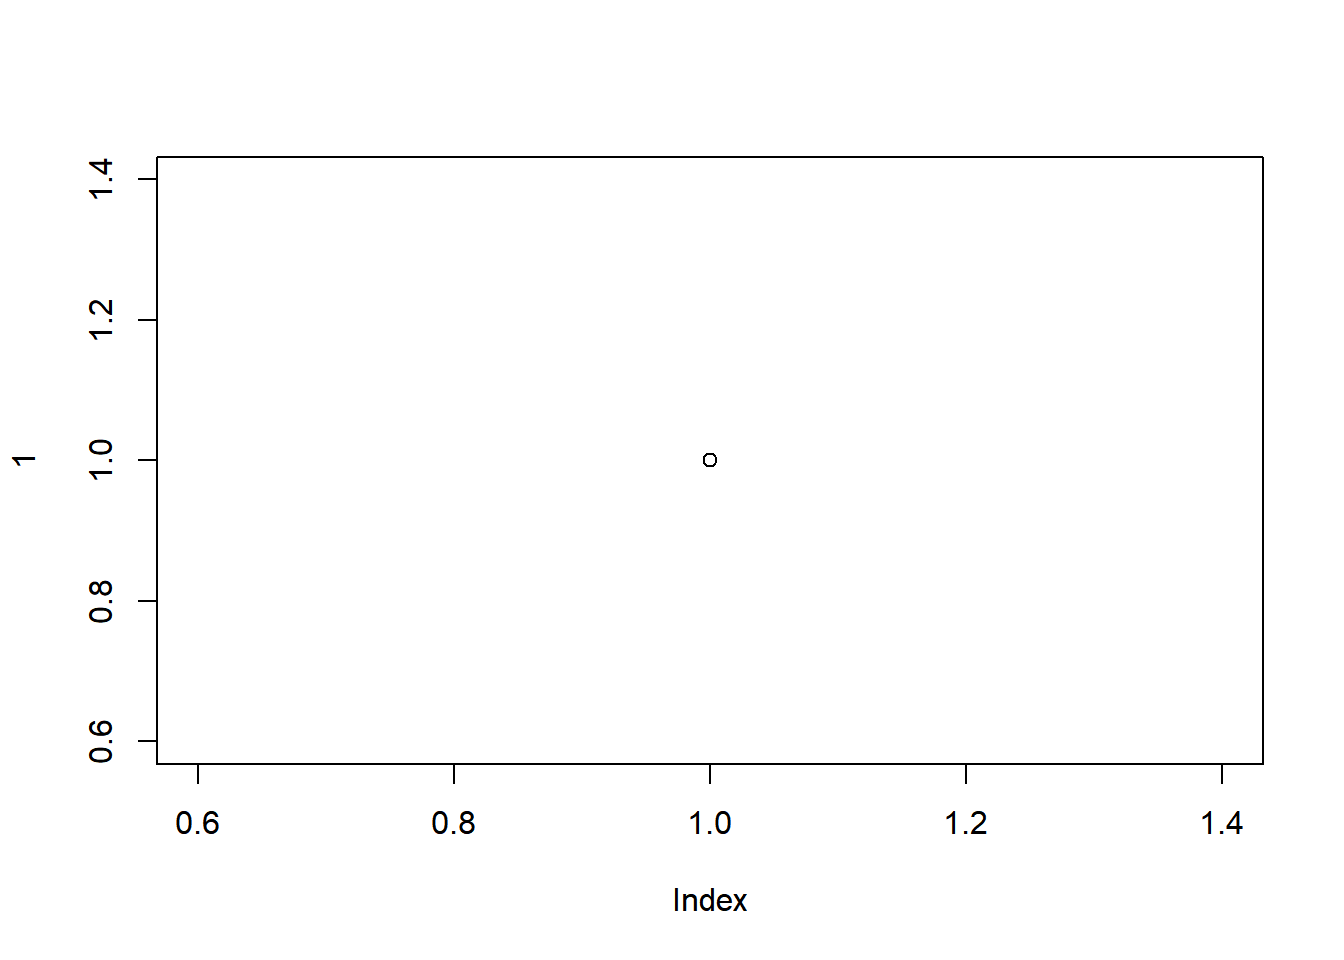
\includegraphics{myRBook_FR_files/figure-latex/unnamed-chunk-102-1.pdf}

\section{hist}\label{hist}

\section{barplot}\label{barplot}

\section{boxplot}\label{boxplot}

\section{image et contour}\label{image-et-contour}

\chapter{La gestion des couleurs}\label{graph2}

\section{colors()}\label{colors}

\section{RGB}\label{rgb}

\section{Paletas}\label{paletas}

\chapter{Graphiques composés}\label{graph3}

\section{mfrow}\label{mfrow}

\section{layout}\label{layout}

\chapter{Manipuler les graphiques}\label{graph4}

\section{Inkscape}\label{inkscape}

\section{The Gimp}\label{the-gimp}

\part{Statistiques}\label{part-statistiques}

\chapter{Statistiques descriptives}\label{stats1}

\part{Etude de cas}\label{part-etude-de-cas}

\chapter{Analyser des données de datalogger de
température}\label{studyCase1}


\end{document}
